%:Clase del documento
\documentclass[fontsize=10pt, English=true, Myfinal=true, twoside, numbers=noenddot]{scrbook}
%Available options (see libroETSI.sty / edicionPFC.sty):
%  Minion=true   - use Minion Pro font (requires the commercial font installed)
%  English=true  - English as main language; Spanish remains available for the
%                  Resumen and the Tribunal page
%  Myfinal=true  - turn off the draft watermark

%:Paquete de estilos propuesto
\usepackage{libroETSI}

%:Paquete específico para cargar tikz (y sus librerías) y pgfplots
\usepackage{dtsc-creafig}

%:Paquete para notaciones específicas
\usepackage{notacion}

%:Paquete para incorporar aspectos concretos de la edición
\usepackage{edicionPFC}

%:Float fencing -- prevents figures from drifting into the wrong section
\usepackage{placeins}
%:Float [H] specifier -- forces figures to render in place (no floating)
\usepackage{float}

%:Push leftover vertical space to the bottom margin (no inter-element stretching)
\raggedbottom


%:Estas líneas de código son INNECESARIAS excepto para mostrar determinadas características en este manual. Pueden eliminarse o comentarse sin ningún problema.
%Se usan para compilar el capítulo estilolibroetsi.tex
\usepackage[final]{showexpl}
\lstset{explpreset={frame=none,rframe={}, numbers=none,numbersep=3pt, columns=flexible,language={[LaTeX]TeX},basicstyle=\ttfamily,keywordstyle=\color{blue}}}%numberstyle=\tiny,

%:Para modificar fácilmente la fuente del texto.
\makeatletter
\ifdtsc@Minion % Queremos utilizar la fuente Minion y lo hemos declarado al principio
	\ifluatex
		\setmainfont[Renderer=Basic, Ligatures=TeX,	% Fuente del texto 
		Scale=1.01,
		]{Minion Pro}
   		% En este caso conviene modificar ligeramente el tamaño de las fuentes matemáticas
		\DeclareMathSizes{10}{10.5}{7.35}{5.25}
		\DeclareMathSizes{10.95}{11.55}{8.08}{5.77}
		\DeclareMathSizes{12}{12.6}{8.82}{6.3}
%		\setmainfont[Renderer=Basic, Ligatures=TeX,	% Fuente del texto 
%		]{Adobe Garamond Pro}
%		\setmainfont[Renderer=Basic, Ligatures=TeX,	% Fuente del texto 
%		]{Palatino LT Std}
	\fi
\else
	\ifluatex
		% Para utilizar la fuente Times New Roman, o alguna otra que se tenga instalada
		\setmainfont[Renderer=Basic, Ligatures=TeX,	% Fuente del texto 
		Scale=1.0,
		]{Times New Roman}
	\else
		\usepackage{tgtermes} 	%clone of Times
		%\usepackage[default]{droidserif}
		%\usepackage{anttor} 	
	\fi
\fi
\makeatother

%Por si quieren usar bibliografía con BIBER
%BIBER%%:Para la bibliografía en BIBER, descomentar las líneas siguientes
%\defbibheading{etsi}[]{%
%	\chapter*{Bibliografía}%
%	\chaptermark{Bibliografía} 
%	\markboth{#1}{#1}}
%\addbibresource{bibliografiaLibroETSI.bib}

% Ejemplo de Glosario
\newacronym[type=main]{ETSI}{ETSI}{Escuela Técnica Superior de Ingeniería}
\newacronym[type=main]{US}{US}{Universidad de Sevilla}
\newacronym[type=main]{DMC}{DMC}{Canal Discreto sin Memoria}


\makeindex
\makeglossaries %Si no se quiere el glosario, comentar esta línea.

% Formato A4
\geometry
{paperheight=297mm,%
paperwidth=210mm,%
top=25mm,%
headsep=8.5mm,%
includefoot, 
textheight=240mm, 
textwidth=150mm, 
bindingoffset=0mm, 
twoside}

\usepackage[a4,center]{crop}%para poner las cruces de esquina de página, poner la opción cross

%:Esquema de numeración por defecto
\setenumerate[1]{label=\normalfont\bfseries{\arabic*.}, leftmargin=*, labelindent=\parindent}
\setenumerate[2]{label=\normalfont\bfseries{\alph*}), leftmargin=*}
\setenumerate[3]{label=\normalfont\bfseries{\roman*.}, leftmargin=*}
\setlist{itemsep=.1em}
\setlength{\parindent}{1.0 em}
\setlength{\parskip}{0.4\baselineskip plus 0.1\baselineskip minus 0.05\baselineskip}

\setcounter{tocdepth}{4}						% El nivel hasta el que se muestra el índice 


%:Empieza el documento

\begin{document}

%PORTADA
%ver edicionPFC.sty para modificaciones

%:Para crear la portada y la portada interior (pagina titular)
\titulo{A Study on Foundational Visual-Language Models \mbox{for } Histopathology Image Analysis} %\mbox evita que se divida una palabra al cambiar de línea
\autor{Leandro Candau Sánchez de Ybargüen}
\director{Miguel Ángel Gutiérrez Naranjo}
\titulodirector{Profesor Titular}
\directorb{Miguel Cárdenas Montes}
\titulodirectorb{Co-director}

\departamento{Dpto. de Ciencias de la Computación e IA}
\centro{Escuela Técnica Superior de Ingeniería Informática}
\universidad{Universidad de Sevilla}
\titulacion{Máster Universitario en Lógica, Computación e IA}
\fecha{2026}
% Keep in Spanish per ETSI submission convention; avoid the English
% label for this work as the school is strict about that.
\nombretrabajo{Trabajo de Fin de Máster}

\hypersetup
	{
 	linkcolor=black, %Tocar para poner color en enlaces
	pdfauthor={\elautor},
	pdftitle={\nombretrabajo,\eltitulo}, 
	pdfkeywords={Latex, edición, formato de texto}	
	 }

\portadaPFC{figuras/LogoUS.pdf}{figuras/LogoTSC.pdf} %logo de la Universidad y logo del departamento, si lo hubiera. Para cambiar el pie de página con los logos, debe editarse el fichero ediciónPFC.sty

%Fin Portada

%FrontMatter
%Todo lo que constituye la primera parte del libro que no es el cuerpo del libro en realidad
\frontmatter
\pagenumbering{Roman} %Pone la numeración en mayúscula (En español parece que es obligatorio)

%Agradecimientos
% !TEX root =../tfmETSI.tex
\chapter*{Agradecimientos}
\pagestyle{empty}
\phantomsection

\lettrine[lraise=-0.1, lines=2, loversize=0.25]{L}{orem} ipsum dolor sit amet, consectetur adipiscing elit. Integer libero leo, imperdiet in sollicitudin a, rutrum ut libero. Aliquam nec mauris rhoncus, volutpat purus id, luctus magna. Phasellus quis leo ut erat malesuada ultricies quis nec massa. Praesent ac cursus felis. Suspendisse potenti. Phasellus volutpat dictum volutpat. Phasellus quis augue nisl. Donec id nunc convallis, maximus erat vel, imperdiet leo. Pellentesque placerat neque vel bibendum blandit. Ut commodo scelerisque nulla, eu bibendum elit porta facilisis. Aliquam erat volutpat. Aenean tempor arcu quis mi iaculis porttitor. Fusce bibendum imperdiet aliquam. Vivamus vitae metus ultricies massa tincidunt dapibus.

Duis luctus arcu ut sem posuere pretium. Ut feugiat, mi eu tempor auctor, sem mi posuere lacus, gravida bibendum tellus sapien non lacus. Aliquam erat volutpat. Donec auctor condimentum varius. Integer sit amet imperdiet ante, nec molestie ipsum. Aenean mauris arcu, consequat feugiat dignissim sed, malesuada vel mi. Nullam egestas non felis ut dictum. Aenean lobortis tristique augue a venenatis. Aenean vestibulum justo ac leo dignissim blandit. Nunc porta sem id risus maximus cursus. Orci varius natoque penatibus et magnis dis parturient montes, nascetur ridiculus mus. Integer ullamcorper lectus justo, sit amet interdum risus bibendum in. Praesent venenatis egestas est in vulputate. Proin id tempor mauris, nec sagittis elit. Maecenas cursus lacus in dignissim sagittis.

{\flushleft{\hfill \emph{Leandro Candau Sánchez de Ybargüen}}}%
\vspace{-.3cm}
{\flushleft{\hfill \emph{Sevilla, 2026}}}%


%TFM
% !TEX root =../tfmETSI.tex

\chapter*{Resumen}
\pagestyle{especial}
\chaptermark{Resumen}
\phantomsection
\addcontentsline{toc}{listasf}{Resumen}

\begin{itemize}
    \item \textbf{Contexto.} Clasificación de imágenes histopatológicas bajo el cuello de botella recurrente del dominio: datos etiquetados limitados y vocabularios de etiquetas estrechos.
    \item \textbf{Enfoque.} Aprendizaje contrastivo imagen--texto al estilo CLIP con codificadores fundacionales congelados. Sobre una línea base controlada (ResNet50 + BERT congelados) se evalúa una matriz de ablaciones de una sola variable, entrenadas en Kaggle LC25000 (5 clases de tejido pulmonar y colónico) y evaluadas tanto sobre LC25000 como sobre tres conjuntos externos no vistos en entrenamiento.
    \item \textbf{Resultado principal.} El \emph{preentrenamiento del codificador de imagen} es, con diferencia, la palanca dominante. Manteniendo el resto del pipeline idéntico y sustituyendo el ResNet50 de propósito general (ImageNet) por el ViT-B/32 preentrenado en histopatología de PLIP, la macro-F1 externa mejora en $+0.067$ en colon de cercanía (NCT-CRC), $+0.027$ en colon de otro hospital (Chaoyang) y $+0.335$ en pulmón de otro órgano (LungHist700).
    \item \textbf{Descomposición con DINOv2.} Un ViT-B/14 con preentrenamiento autosupervisado en imágenes naturales generales (sin histopatología) eleva LungHist700 en $+0.152$ sobre la línea base --- aproximadamente la mitad de la ganancia de PLIP. La otra mitad procede del preentrenamiento específico en histopatología.
    \item \textbf{Hallazgos secundarios.} De las otras cinco intervenciones probadas, la normalización de tinción Macenko (referencia NCT-NORM) es la única palanca del lado de la entrada que produce una ganancia positiva medible bajo desplazamiento ($+0.030$ en Chaoyang, $+0.020$ en LungHist700), pero su magnitud queda dominada por la palanca del codificador de imagen en los mismos conjuntos y regresa en NCT-CRC ($-0.022$, que llega ya normalizado por Macenko en su \emph{release}). Los codificadores de texto biomédicos, el clasificador de entropía cruzada sin CLIP y las variaciones de formato de \emph{prompt} no mejoran la generalización. La ventaja de CLIP sobre un clasificador no-CLIP aparece sólo bajo desplazamiento más fuerte, vía la geometría \emph{coseno + L2-normalizada + escalada por temperatura} del clasificador.
    \item \textbf{Aporte metodológico.} El reporte por órgano es esencial: agregar los conjuntos externos en un único número promedio oculta el cambio de régimen entre colon (transferencia parcial con ResNet50/ImageNet congelado) y pulmón (fallo categórico del mismo \emph{backbone}).
\end{itemize}


\chapter*{Abstract}
\pagestyle{especial}
\chaptermark{Abstract}
\phantomsection
\addcontentsline{toc}{listasf}{Abstract}

\begin{itemize}
    \item \textbf{Context.} Histopathology image classification under the domain's recurring bottleneck: limited labelled data and narrow label vocabularies.
    \item \textbf{Approach.} CLIP-style image--text contrastive learning with frozen foundation-model encoders. A single-variable ablation matrix is evaluated over a controlled baseline (frozen ResNet50 + frozen BERT), trained on Kaggle LC25000 (5 lung and colon tissue classes) and evaluated on both LC25000 and three additional external datasets the model has never seen.
    \item \textbf{Headline result.} The \emph{image encoder's pretraining} is by far the dominant lever. Holding the rest of the pipeline identical and swapping the general-purpose ResNet50 (ImageNet) for PLIP's histopathology-pretrained ViT-B/32 lifts external macro-F1 by $+0.067$ on close-shift colon (NCT-CRC), $+0.027$ on different-hospital colon (Chaoyang), and $+0.335$ on different-organ lung (LungHist700).
    \item \textbf{DINOv2 decomposition.} A ViT-B/14 with self-supervised pretraining on general natural images (no histopathology data) lifts LungHist700 by $+0.152$ over baseline --- roughly half of PLIP's gain. The other half comes from histopathology-specific pretraining.
    \item \textbf{Secondary findings.} Among the other five interventions tested, Macenko stain normalization (NCT-NORM reference) is the only input-side lever that produces a measurable positive gain under shift ($+0.030$ on Chaoyang, $+0.020$ on LungHist700), but its magnitude is dominated by the image-encoder lever on the same datasets and it regresses on NCT-CRC ($-0.022$, which arrives Macenko-normalised at release). Biomedical text encoders, a non-CLIP cross-entropy classifier, and prompt-format variations do not improve generalization. CLIP's edge over a non-CLIP classifier appears only under heavier shift, via the \emph{bounded-cosine + L2-normalised + temperature-scaled} classifier geometry.
    \item \textbf{Methodological contribution.} Per-organ external reporting is essential: aggregating external datasets into a single mean-OOD number hides the regime change between colon (partial transfer with a frozen ImageNet ResNet50) and lung (categorical failure of the same backbone).
\end{itemize}
 

%Índice normal, el completo
\cleardoublepage
\phantomsection
\pagestyle{especial}
\tableofcontents

%Fin FrontMatter

%Texto Principal
\mainmatter

%:Página por defecto
\pagestyle{esitscCD}

%:Los diferentes capítulos, en carpetas separadas

%Chapter 1: Introduction
% !TEX root =../tfmETSI.tex
\chapter{Introduction}\label{chp:introduction}
\epigraph{Learning directly from raw text about images is a promising alternative which leverages a much broader source of supervision.}{Radford et al., 2021}

\section{Motivation}
\label{sec:intro-motivation}

Histopathology --- the microscopic examination of stained tissue sections --- is the gold-standard test for the definitive diagnosis of cancer and many other diseases~\cite{vanderlaak2021deeplearning}. Automating any meaningful part of the pathologist's workflow (triaging slides, flagging regions of interest, suggesting a candidate diagnosis) is one of the highest-impact targets for medical AI, and the visual patterns involved are well-defined enough to be machine-learnable in principle.

The practical bottleneck is data. Labelled histopathology is expensive to produce --- it takes pathologist time and clinical context that do not scale --- and patient privacy further restricts what can be shared. This makes any approach that relies on broad, label-cheap supervision particularly attractive.

Foundation models~\cite{bommasani2021foundation} are designed for exactly this regime: models trained on broad data at large scale that can then be adapted to a wide range of downstream tasks with little task-specific supervision. In the vision--language line, CLIP~\cite{radford2021clip} is the canonical example and the paradigm under study in this work. In plain terms, CLIP trains two encoders side by side, one for images and one for text, so that matched image--text pairs land close together in a shared embedding space. Once trained, the model can be applied to a new classification task simply by writing a short text prompt for each class, with no further training required. We unpack the architecture and training signal in Chapter~\ref{chp:methodology}; for now it is enough to know that CLIP is the closest thing to a general-purpose vision--language model available off the shelf.

Within the same paradigm, the histopathology-specific variant we use in this work is \textbf{PLIP}~\cite{huang2023plip}: the same dual-encoder contrastive recipe, trained on $\sim 208$k pathology image--text pairs scraped from medical Twitter. PLIP is one of several histopathology foundation models available (the broader family is reviewed in Chapter~\ref{chp:stateofart}), and we pick it here because it is the closest single-variable swap from our baseline: same CLIP architecture, ViT-B compute footprint, and openly released weights. PLIP plays two roles in this work: as a zero-shot reference for what an off-the-shelf domain-pretrained model can do without any task-specific training, and as the histopathology-pretrained image encoder swapped into the main pipeline in Chapter~\ref{chp:results}, where it produces the headline finding.

\textbf{The question this project asks is where the pretraining of a CLIP-style histopathology pipeline actually pays off, and where it does not} --- evaluated across head-side, loss-side, text-side, and image-side interventions, both in-distribution and on three external datasets covering two organs. The framing is deliberate: CLIP as the object of study rather than the classifier itself, so the findings should generalise to other scientific domains where short or missing labels are the norm.


\section{Project Scope Evolution}
\label{sec:intro-scope}

The project began with a different scope. The initial direction was semantic segmentation of histopathology slides --- pixel-level identification of tissue regions --- which is closer to what a clinical workflow actually produces. That direction was abandoned within the first few weeks: annotated segmentation data at the scale we needed was too scarce, and producing it would have required pathologist time well beyond the project budget. We pivoted to image-level classification on the same domain, which preserves the methodological questions about CLIP and histopathology while removing the data-cost wall.

The training source is LC25000~\cite{borkowski2019lc25000}, a 5-class lung-plus-colon patch dataset that fits the frozen-backbone training regime without needing pixel-level labels. External evaluation runs on three datasets chosen to span shift severity and two organs: NCT-CRC-HE-7K~\cite{kather2019nct} (close-shift colon), Chaoyang~\cite{zhu2021chaoyang} (different-hospital colon), and LungHist700~\cite{tabatabaei2024lunghist} (different-source lung). The study is organised as a series of single-variable comparisons: each experiment changes exactly one component of a fixed baseline (frozen ResNet50 + frozen BERT with a CLIP head trained on top) --- the image encoder, the text encoder, the input preprocessing, or the classifier head --- and holds the rest identical. The delta on each external dataset then traces back to one specific design decision, and the comparisons that follow in Chapter~\ref{chp:results} tell us which of those decisions actually matter.


\section{Research Questions}
\label{sec:intro-rq}

The work is structured around six research questions. \textbf{The central one is cross-cutting}: how does a CLIP-style histopathology pipeline generalise to data the model has never seen? The other five each isolate a single axis of the pipeline (baseline behaviour, the CLIP-vs-non-CLIP architecture choice, input preprocessing, the text encoder, and the image encoder) so that the contribution of each can be measured separately when answering this cross-cutting question.

\begin{itemize}
    \item \textbf{RQ1} --- What baseline classification and generalisation behaviour does a frozen general-purpose CLIP pipeline (ImageNet ResNet50 + BERT) achieve on LC25000, and what failure modes appear?
    \item \textbf{RQ2} --- Does the CLIP paradigm validate its \emph{foundational-model} premise relative to a non-CLIP classifier on the same image encoder, both in-distribution and on data the model was never trained on?
    \item \textbf{RQ3} --- Does stain normalisation help when we evaluate on datasets the model was never trained on?
    \item \textbf{RQ4} --- Does using a text encoder pretrained on biomedical text (BioBERT~\cite{lee2020biobert}, PubMedBERT~\cite{gu2021pubmedbert}), instead of generic BERT~\cite{devlin2019bert}, improve performance? And does the prompt format (bare class name vs longer composed prompt) interact with the encoder choice?
    \item \textbf{RQ5} --- Does the image encoder's \emph{pretraining choice} matter? Specifically: replacing the general-purpose ResNet50~\cite{he2016resnet} with PLIP's histopathology-pretrained ViT-B/32~\cite{huang2023plip,dosovitskiy2021vit}, and with DINOv2's general-domain self-supervised ViT-B/14~\cite{oquab2024dinov2} (a strong off-the-shelf image encoder trained without labels on $\sim 142$M general natural images) as a control that isolates ``ViT architecture and self-supervision'' from ``histopathology pretraining specifically''.
    \item \textbf{RQ6} --- How well does each variant generalise to data the model has never seen, evaluated across three external datasets that span shift severity and two organs?
\end{itemize}


\section{Contributions}
\label{sec:intro-contributions}

The central contribution of this project is a controlled measurement of how much each major design choice in a CLIP-style histopathology pipeline actually matters, with every claim framed as a delta over the same baseline --- frozen ResNet50 + frozen BERT, single fixed prompt, stratified 80/10/10 split on LC25000 --- and iterated through one experiment at a time in Chapter~\ref{chp:results}.

Headline findings (full results in Chapter~\ref{chp:results}):
\begin{itemize}
    \item \textbf{Image encoder pretraining is the dominant lever.} Replacing ResNet50 with PLIP's pretrained ViT-B/32 (histopathology image--text contrastive) gains $+0.067$ F1 on close-shift colon (NCT-CRC), $+0.027$ on different-hospital colon (Chaoyang), and $+0.335$ on different-source lung (LungHist700). No other intervention tested moves the needle comparably.
    \item \textbf{The lung-side advantage decomposes into three additive steps of comparable magnitude.} The DINOv2 and PLIP zero-shot controls together decompose PLIP's $+0.335$ F1 lung advantage into three contributions: ViT + self-supervised pretraining on general images ($+0.152$), histopathology pretraining specifically ($+0.087$), and LC25000 supervision on top ($+0.096$).
    \item \textbf{Five other interventions move the needle far less, or only in narrow regimes.} Stain Macenko (NCT-NORM reference) is the only input-side lever that produces a measurable positive gain under shift ($+0.030$ on Chaoyang, $+0.020$ on LungHist700), but its magnitude is dominated by the image-encoder lever on the same datasets and it regresses on NCT-CRC ($-0.022$, which arrives Macenko-normalised at release). Biomedical text encoders (BioBERT, PubMedBERT) tie or trail baseline across all 6 grid cells on NCT, and the best biomedical cell (PubMedBERT + name\_only) extended to Chaoyang and LungHist700 confirms no transfer benefit on any of the three datasets. A non-CLIP plain classifier ties CLIP in-distribution and on close-shift external data but loses on heavier shift; prompt-format variations within the text-encoder comparison are within noise.
    \item \textbf{CLIP's foundational-model premise is validated under shift, not in-distribution.} CLIP and a plain CE classifier tie at saturation in-distribution and on close-shift external; CLIP's edge appears under heavier shift via the bounded-cosine + temperature-scaled classifier geometry, which does not degenerate the way high-confidence softmax does.
\end{itemize}

Methodological contributions:
\begin{itemize}
    \item Single-variable-change protocol: each experiment differs from the baseline in exactly one design choice, so the resulting delta is attributable.
    \item Per-organ external reporting: results are presented per dataset, not averaged; averaging across datasets would hide the cross-organ regime change observed in this study.
    \item Reproducibility: artifact bundle (fixed-seed split, cached DINOv2 features, weights, metric files, plots) versioned alongside the report in the project repository.
    \item Explicit written discussion of dataset and methodological limits (Chapter~\ref{chp:conclusion}).
\end{itemize}


\section{Document Structure}
\label{sec:intro-structure}
\begin{itemize}
    \item Chapter~\ref{chp:introduction} (Introduction) --- motivation, scope, research questions, contributions.
    \item Chapter~\ref{chp:stateofart} (State of the Art) --- foundation models, multimodal contrastive lineage, pathology FMs, where this work fits.
    \item Chapter~\ref{chp:methodology} (Methodology) --- CLIP architecture, image and text encoders, datasets, preprocessing, baseline, evaluation protocol, reproducibility.
    \item Chapter~\ref{chp:results} (Results and Discussion) --- the experiments and what each measured, ending in a synthesis section.
    \item Chapter~\ref{chp:conclusion} (Conclusions and Future Work) --- one-paragraph-per-RQ conclusions, limitations, future work.
\end{itemize}


%Chapter 2: State of the Art
% !TEX root =../tfmETSI.tex
\chapter{State of the Art}\label{chp:stateofart}
\epigraph{AI is undergoing a paradigm shift with the rise of models [...] that are trained on broad data at scale and are adaptable to a wide range of downstream tasks.}{Bommasani et al., 2021}

% Single flowing narrative, ~3 pages once written. Focused on histopathology
% foundation models. Deep-learning lineage covered in Methodology.

\begin{itemize}
    \item Foundation models framing (Bommasani 2021).
    \item CLIP and multimodal contrastive learning (Radford 2021) --- the paradigm under study.
    \item Self-supervised visual pretraining for medical imaging --- DINO, DINOv2.
    \item Pathology shift: per-tile supervised CNNs $\to$ foundation models (2016--2024).
    \item Pathology-specific foundation models:
    \begin{itemize}
        \item TransPath (2022) --- transformer + SSL.
        \item Phikon (2023) --- masked image modelling.
        \item PLIP (2023) --- CLIP on medical Twitter.
        \item CONCH (2024) --- larger pathology VLM.
        \item BiomedCLIP, MUSK --- recent entrants.
    \end{itemize}
    \item Open challenges: benchmarks, dataset bias, cross-institution generalization, compute scale.
    \item Where this project fits: small-scale empirical study of general-purpose foundation backbones on pathology classification, with single-variable ablations.
\end{itemize}


%Chapter 3: Methodology
% !TEX root =../tfmETSI.tex
\chapter{Methodology}\label{chp:methodology}

\section{Overview}
\label{sec:meth-overview}

The chapter sets up the building blocks the rest of this work rests on: the contrastive vision-language paradigm under study (CLIP, §\ref{sec:meth-clip}), the encoders we plug into it (§\ref{sec:meth-image}, §\ref{sec:meth-text}), the training and external-evaluation datasets (§\ref{sec:meth-dataset}, §\ref{sec:meth-external-datasets}), the preprocessing and baseline configuration (§\ref{sec:meth-pre}, §\ref{sec:meth-baseline}), and the evaluation protocol that all experiments share (§\ref{sec:meth-eval}). The chapter ends with the compute and reproducibility setup (§\ref{sec:meth-compute}). Two reference baselines (PLIP zero-shot and a non-CLIP plain image classifier) run alongside the main experiment matrix; their configurations are described inline in the Results chapter where each is evaluated (§\ref{sec:results-plip-zeroshot}, §\ref{sec:results-foundational-vs-plain}).

The structure is intended to be read linearly --- background first, then the baseline configuration, then the experiments. Every experiment in the chapters that follow uses a single-variable-change design: each variant changes exactly one component of the baseline (image encoder, text encoder, input preprocessing, classifier head, or prompt format) and holds everything else identical, so that any observed delta on external evaluation traces back to that single change. The full experiment matrix --- which variant changes which axis --- is given in Table~\ref{tab:experiment-matrix} of Chapter~\ref{chp:results}.

Before going further, it is worth being clear about what this work does not attempt. We do not work with patient-level groupings (LC25000 is not patient-grouped), we do not run human-expert or clinical evaluation, and we do not include a controlled head-to-head against other histopathology foundation models (CONCH~\cite{lu2024conch}, BiomedCLIP~\cite{zhang2023biomedclip}, MUSK~\cite{xiang2025musk}). All three are listed as future work in Chapter~\ref{chp:conclusion}.


\section{Histopathology Digital Imaging}
\label{sec:meth-histo}

\subsection{Background}

Histopathology is the microscopic study of tissue removed from a patient to diagnose disease --- most commonly cancer. A biopsy or surgical specimen is fixed, embedded in paraffin, sliced into thin sections (typically 4--5\,µm), stained, and mounted on a glass slide for a pathologist to examine under a microscope. The pathologist's report is the gold-standard diagnosis that drives treatment decisions in oncology and many other specialties. Automating any meaningful part of this workflow --- triaging slides, flagging regions of interest, suggesting a diagnosis --- is one of the highest-impact targets for medical AI, both because pathologist time is a scarce resource and because the visual patterns involved are well-defined enough to be machine-learnable.

The stain used almost universally is hematoxylin and eosin (H\&E): hematoxylin colours cell nuclei a dark blue/purple, eosin colours cytoplasm and extracellular matrix pink. Slides are digitised by a Whole-Slide Imaging (WSI) scanner into a multi-gigapixel image (Figure~\ref{fig:wsi-multimag}), which is typically tiled into smaller patches (commonly $224 \times 224$ or $512 \times 512$ pixels at $20\times$ or $40\times$ magnification) for downstream learning, since current image encoders cannot process whole slides directly. Figure~\ref{fig:nct-crc-classes} shows the tissue-type variation a model has to discriminate between within a single dataset.

\begin{figure}[H]
    \centering
    \includegraphics[width=0.95\textwidth]{../results/plots/methodology/external/wsi_he_multimag_wikimedia.png}
    \caption{An H\&E-stained whole-slide image of breast tumour tissue at three magnification levels ($4\times$, $20\times$, $40\times$) over a $2.2$~cm$^2$ area. The slide-level view shows tissue architecture; higher magnifications reveal cellular detail used by pathologists for diagnosis. Image by KajsaMollersen, 2022; reproduced under CC-BY-SA 4.0.}
    \label{fig:wsi-multimag}
\end{figure}

\begin{figure}[H]
    \centering
    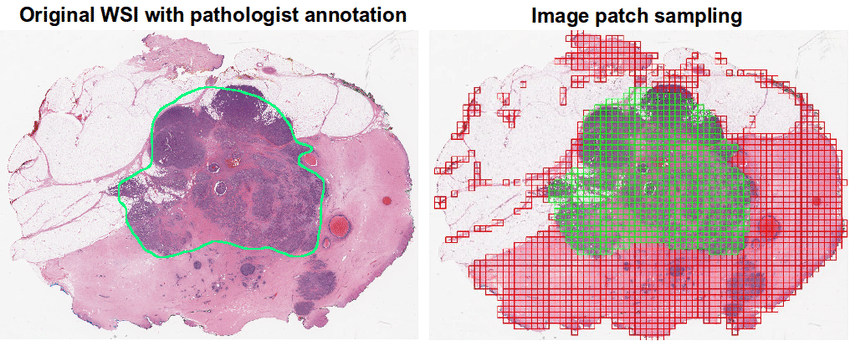
\includegraphics[width=0.85\textwidth]{../results/plots/methodology/external/wsi_patching_cruzroa2014.png}
    \caption{Patch-sampling on a whole-slide image. Left: original WSI with pathologist annotation (green outline) marking the cancer region. Right: the same WSI tiled into patches for downstream learning, with patch tiles intersecting the annotation marked in green and the rest in red. Reproduced from Cruz-Roa et al.~\cite{cruzroa2014idc}.}
    \label{fig:wsi-patching}
\end{figure}

\begin{figure}[H]
    \centering
    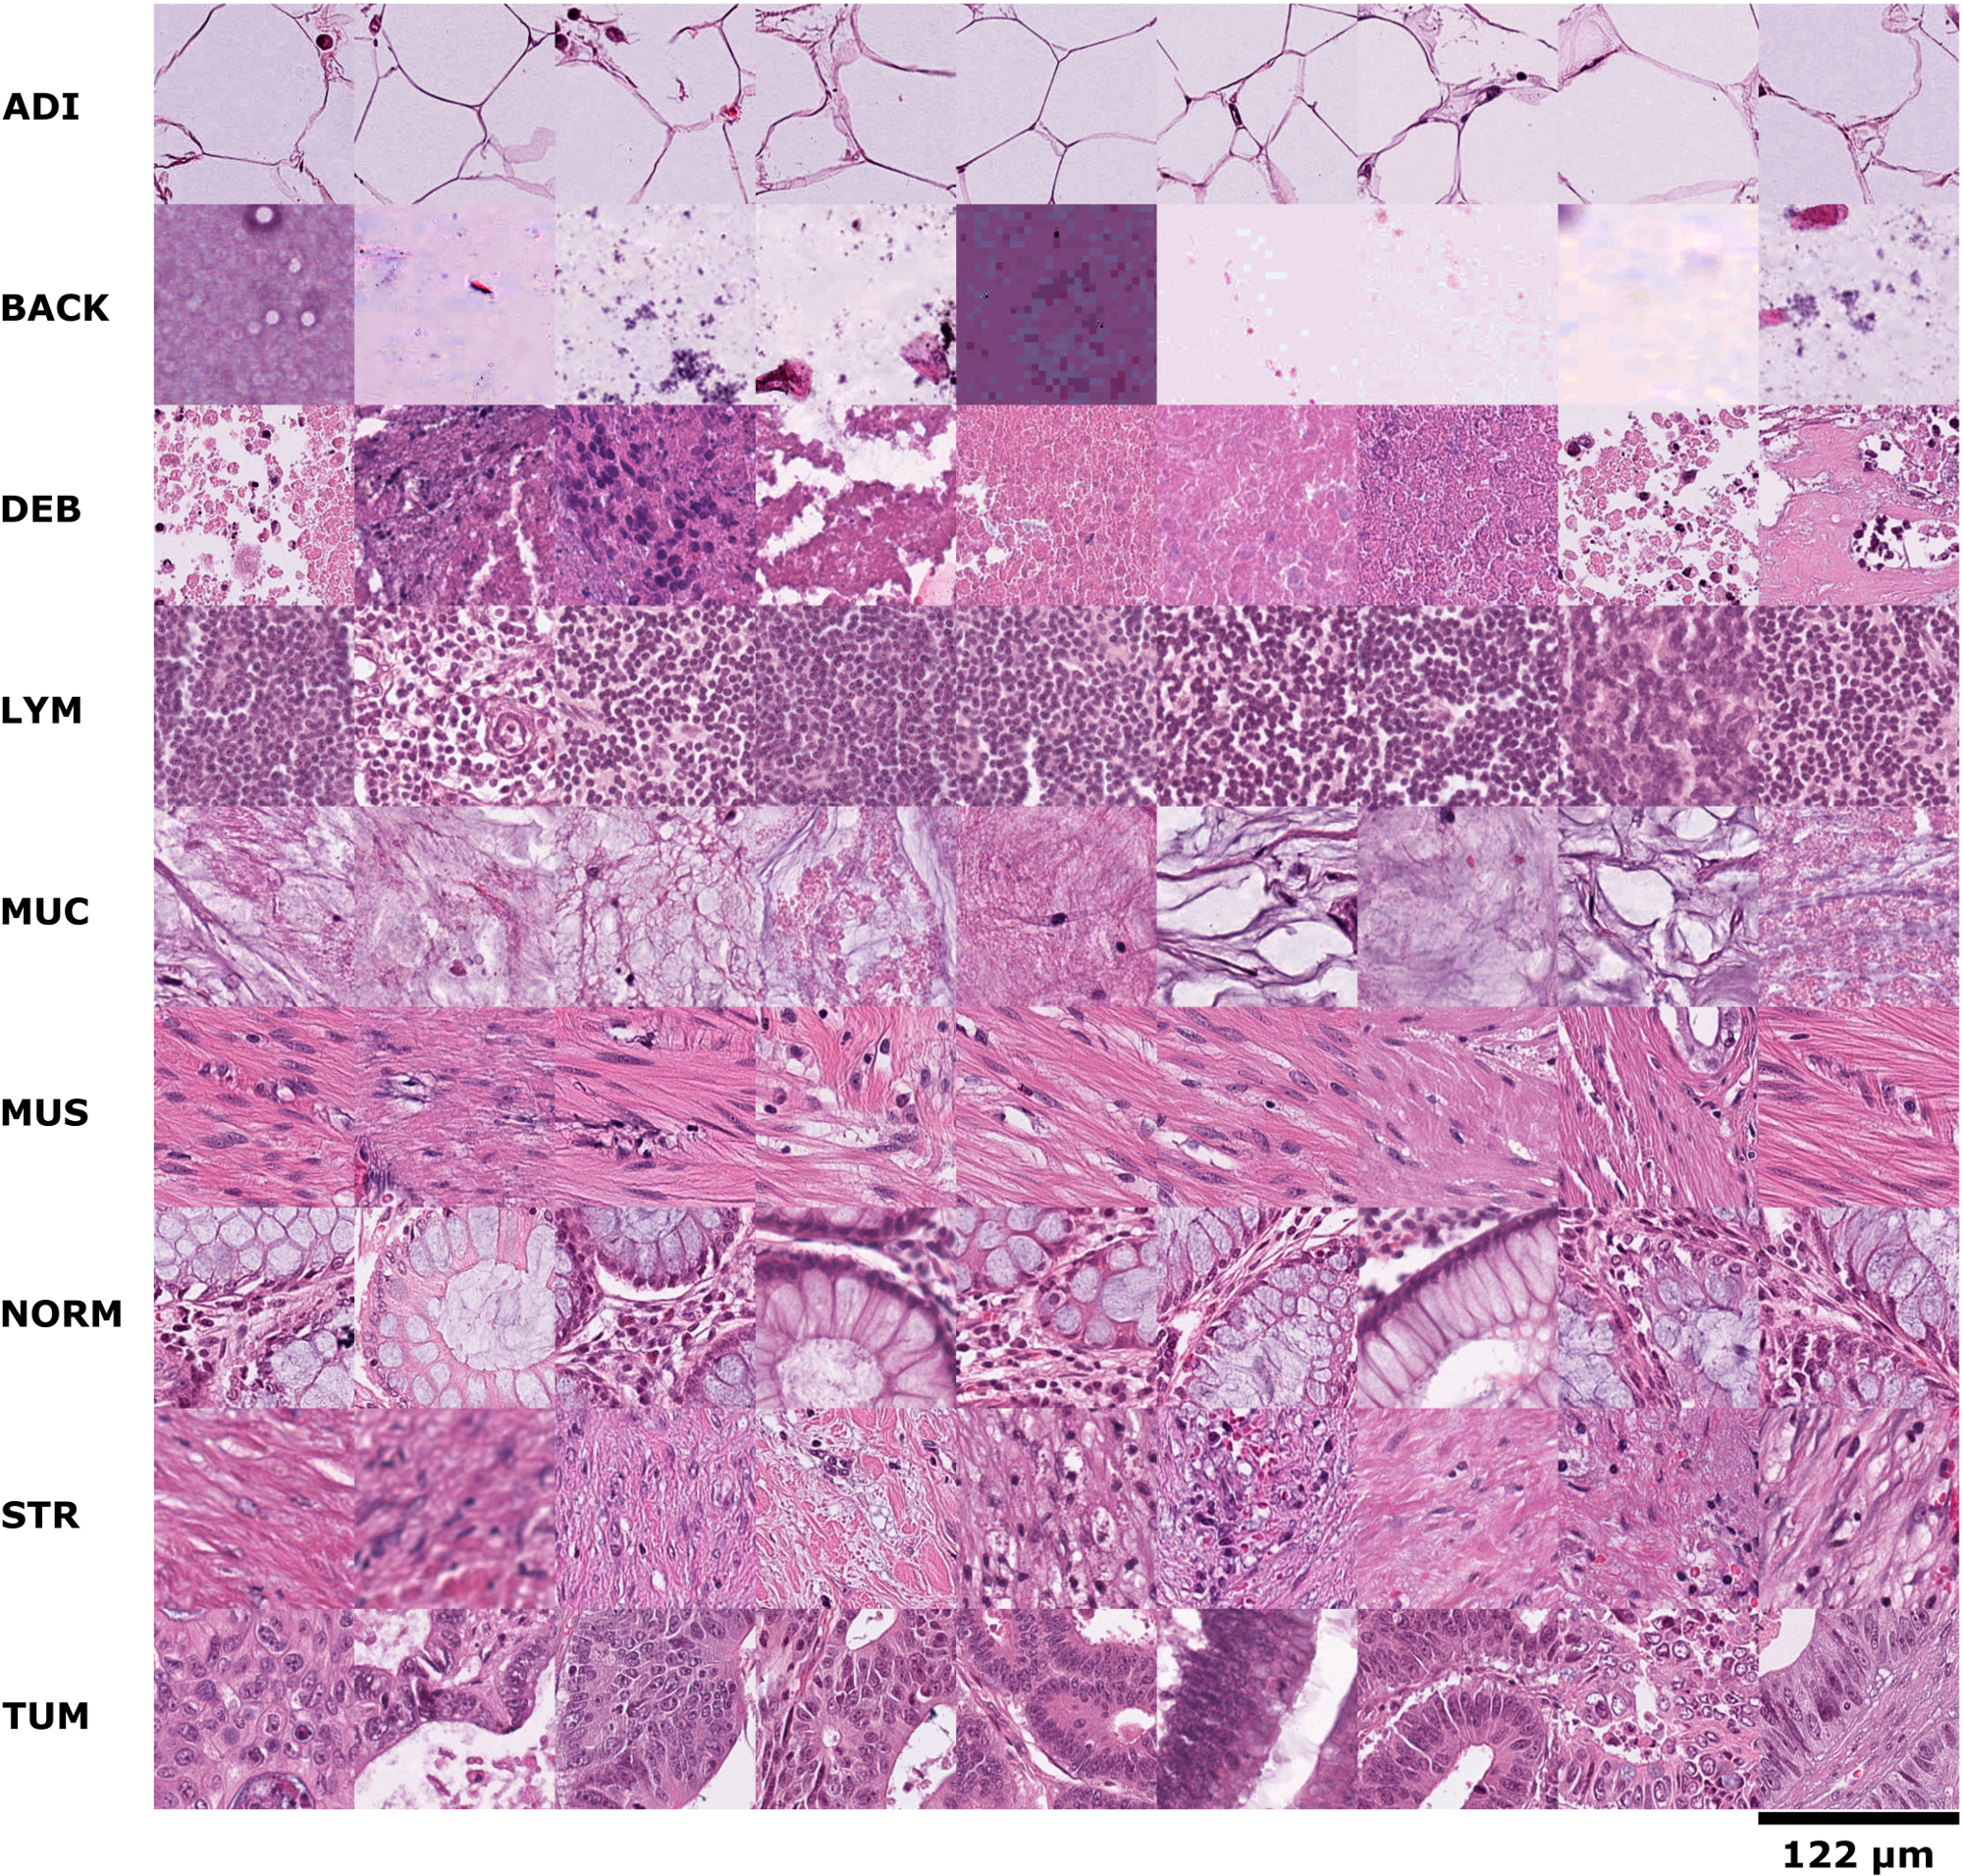
\includegraphics[width=0.85\textwidth]{../results/plots/methodology/external/nct_crc_classes_kather2019.png}
    \caption{Example H\&E patches from each of the nine tissue classes in the NCT-CRC-HE-100K dataset, illustrating the visual variation a histopathology classifier has to discriminate between within a single colorectal-cancer corpus. Figure~1 of Kather et al.~\cite{kather2019nct}, reproduced under the CC-BY 4.0 licence.}
    \label{fig:nct-crc-classes}
\end{figure}

\FloatBarrier

Several things make this domain hard for general-purpose vision-language models. Clinical archives rarely come with per-image natural-language captions of the kind that train CLIP at scale; pathology image--text corpora are small (PLIP's OpenPath has $\sim 208$k pairs, vs CLIP's $400$M for natural images) and noisier in their text. Several public histopathology datasets ship with subtle artifacts --- white-pixel skew, scanner-specific JPEG signatures, augmentation-pair leakage --- that can drive in-distribution performance without any meaningful tissue signal, motivating careful external evaluation. And finally, the visual signature of an H\&E slide depends heavily on the lab and scanner that produced it; that is the topic of the next subsection.

\subsection{Stain normalization in histopathology images}
\label{sec:meth-stain}

H\&E staining is not a deterministic procedure. The hematoxylin and eosin formulations, staining times, scanner colour profiles, and even individual technician handling all introduce variation in the resulting colour palette. Across institutions the variation is large and visible to the eye --- two slides of the same tissue type can look stylistically very different. Within a single institution it is smaller but still present, varying with technician shift, batch of reagents, and scanner calibration. This becomes a problem for any downstream classifier: a model trained on one institution's slides can latch onto that institution's specific stain signature rather than the underlying tissue pattern, then fail on a differently-stained slide of the same disease at evaluation time. Stain normalisation is the family of techniques that tries to remove the confounder by mapping every input into a common reference stain palette before downstream encoding.

Three normalisation methods are commonly cited: Macenko (stain-vector decomposition via SVD on the optical-density-transformed image)~\cite{macenko2009stain}, Reinhard (Lab-space colour-statistics transfer)~\cite{reinhard2001color}, and Vahadane (sparse non-negative matrix factorisation)~\cite{vahadane2016structure}. Figure~\ref{fig:stain-illustration} shows the same LC25000 patch under raw stain and each of the three normalisations --- the colour palette shifts visibly between methods, even though the underlying tissue content is identical. Macenko is the only method we advance to full external evaluation in this work. Reinhard and Vahadane were explored in an early pass but did not move forward: Vahadane's non-negative matrix factorisation solver fails to converge on a non-trivial fraction of LC25000 patches (see §\ref{sec:results-stain}, Figure~\ref{fig:stain-before-after}, for the full multi-class breakdown), and Reinhard is a Lab-space colour-statistics transfer rather than a true stain-decomposition method --- useful as a visual reference but not equivalent to Macenko's stain-vector approach.

Macenko's procedure operates in \textbf{optical-density (OD) space}. An RGB pixel intensity $I \in [0, 255]^3$ is first mapped to OD space by
\begin{equation}
\mathrm{OD} = -\log_{10}\!\left(\frac{I + 1}{I_0}\right), \qquad I_0 = 255,
\end{equation}
where the $+1$ avoids the singularity on pure-black pixels. In OD space, the two stains act as additive components, so each pixel decomposes as
\begin{equation}
\mathrm{OD} = S \cdot C,
\end{equation}
with $S \in \mathbb{R}^{3 \times 2}$ the stain-vector matrix (one 3-D colour vector per stain) and $C \in \mathbb{R}^{2}$ the per-stain concentration. Macenko estimates $S$ from the image by taking the SVD of the OD-space pixel cloud and choosing the two extreme directions in the top-2 singular-vector plane; the concentrations $C$ then follow by pseudo-inversion, $C = S^{+}\, \mathrm{OD}$. To normalise to a reference image with stain matrix $S_\mathrm{ref}$, the concentrations are preserved and re-projected through the reference stains:
\begin{equation}
\mathrm{OD}' = S_\mathrm{ref} \cdot C, \qquad I' = I_0 \cdot 10^{-\mathrm{OD}'}.
\end{equation}
Concretely, the procedure first \emph{learns} what colours the hematoxylin and eosin stains take in the input image, decomposes each pixel into those two components, and then re-renders the pixel using the colours those same stains take in the reference image.

\begin{figure}[H]
    \centering
    \begin{minipage}[t]{0.23\textwidth}
        \centering
        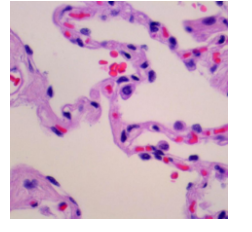
\includegraphics[width=\textwidth]{../results/plots/stain_single_raw.png}
        \par\vspace{2pt}\footnotesize (a) Raw.
    \end{minipage}\hfill
    \begin{minipage}[t]{0.23\textwidth}
        \centering
        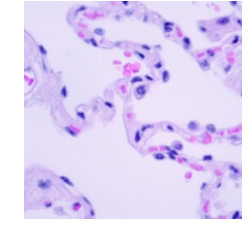
\includegraphics[width=\textwidth]{../results/plots/stain_single_macenko.png}
        \par\vspace{2pt}\footnotesize (b) Macenko.
    \end{minipage}\hfill
    \begin{minipage}[t]{0.23\textwidth}
        \centering
        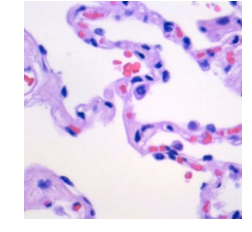
\includegraphics[width=\textwidth]{../results/plots/stain_single_reinhard.png}
        \par\vspace{2pt}\footnotesize (c) Reinhard.
    \end{minipage}\hfill
    \begin{minipage}[t]{0.23\textwidth}
        \centering
        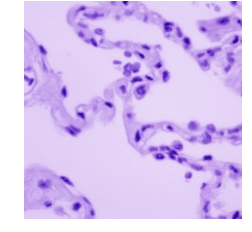
\includegraphics[width=\textwidth]{../results/plots/stain_single_vahadane.png}
        \par\vspace{2pt}\footnotesize (d) Vahadane.
    \end{minipage}
    \caption{Stain normalization comparison on a single LC25000 benign-lung patch. (a) Raw input, (b) Macenko-normalized, (c) Reinhard-normalized, (d) Vahadane-normalized. Each method produces a different colour palette from the same underlying tissue content. The full multi-class comparison, including the Vahadane convergence failure on some patches, is in §\ref{sec:results-stain}.}
    \label{fig:stain-illustration}
\end{figure}

\FloatBarrier

The reference patch is the first \texttt{NORM} tile from NCT-CRC-HE-7K, referred to as ``NCT-NORM'' throughout. Training applies Macenko(NCT-NORM) to every LC25000 patch before the encoder, which lands the training distribution near NCT-CRC's release stain space. At inference, the same Macenko(NCT-NORM) transform is applied to Chaoyang and LungHist700 (both arrive in their native stain palette), but NCT-CRC is fed raw: because NCT-CRC is already Macenko-normalised by Kather et al.~\cite{kather2019nct} before release, applying a second Macenko pass at inference would re-introduce a double-Macenko artefact that zeroed out performance in an earlier version of this experiment. The data-dependent direction this setup produces on external evaluation is the subject of §\ref{sec:results-stain}.


\section{Contrastive Vision-Language Learning (CLIP)}
\label{sec:meth-clip}

\subsection{Why CLIP?}

CLIP~\cite{radford2021clip} (Contrastive Language--Image Pretraining, Radford et al., 2021) is the contrastive vision-language paradigm under study in this work. Originally trained on $\sim 400$M image--text pairs scraped from the web, it learns to associate images with their natural-language descriptions in a shared embedding space and has become one of the most widely-used vision-language foundation models. The reason to centre the project on CLIP rather than on, say, a CNN with a softmax head is that CLIP's training signal --- aligning images with natural-language descriptions in a shared embedding space --- gives the model capabilities a closed-set classifier does not have. Three are directly relevant to histopathology classification:

\begin{itemize}
    \item \textbf{Open-vocabulary classification.} A new class can be introduced at inference time simply by writing a prompt for it; no retraining or label remapping is required. This is the property that lets CLIP be applied zero-shot to datasets it was never trained on.
    \item \textbf{Semantic similarity as the output.} CLIP returns a cosine-similarity score between an image and any text query --- not just a class label --- which makes retrieval and prompt-tuning natural downstream tasks.
    \item \textbf{Prompt engineering as a sensitivity lever.} Because classification depends on how each class is described in natural language, the prompt format itself becomes a tunable knob; we test this directly in §\ref{sec:results-text-encoder}.
\end{itemize}

A practical consequence is that CLIP is the \emph{object} of study in this work rather than the classifier per se. Every variant is evaluated via classification F1, but the broader question is what kind of representations CLIP produces under histopathology supervision, and what changes when individual components of the pipeline are swapped.

\subsection{Architecture and training signal}

The CLIP architecture is a dual-encoder (Figure~\ref{fig:clip-paradigm}): an image encoder and a text encoder, trained jointly so that matched image--text pairs land close together in a shared $d$-dimensional embedding space. Throughout this work we use $d = 256$, the dimensionality of the trained projection head's output. At inference, a sample is classified by encoding the image and each candidate class prompt, then taking the argmax of the cosine similarity between the image embedding and the class-prompt embeddings.

\noindent\textbf{InfoNCE loss.} For a batch of $N$ matched image--text pairs $\{(I_i, T_i)\}_{i=1}^{N}$, the model embeds each side into the shared $d$-dimensional space and produces two L2-normalised batches of embeddings, $\{\mathbf{v}_i\}$ and $\{\mathbf{t}_i\}$. Define the scaled cosine similarity between image $i$ and prompt $j$ as
\begin{equation}
s_{ij} \;=\; \frac{\mathbf{v}_i \cdot \mathbf{t}_j}{\tau},
\label{eq:scaled-cosine}
\end{equation}
where $\tau$ is the learnable temperature introduced below. For each image $i$ the image-to-text contrastive loss treats the matched prompt $i$ as the positive and the other $N{-}1$ prompts in the same batch as negatives; the row-wise softmax cross-entropy then reads
\begin{equation}
\mathcal{L}_{I \to T} \;=\; -\frac{1}{N} \sum_{i=1}^{N} \log \frac{\exp(s_{ii})}{\sum_{j=1}^{N} \exp(s_{ij})}.
\label{eq:infonce-i2t}
\end{equation}
The symmetric InfoNCE loss~\cite{oord2018cpc,radford2021clip} averages this with the analogous column-wise text-to-image loss $\mathcal{L}_{T \to I}$ (in which each prompt is matched against its image positive and the $N{-}1$ batch images as negatives):
\begin{equation}
\mathcal{L}_{\text{InfoNCE}} \;=\; \tfrac{1}{2} \left( \mathcal{L}_{I \to T} + \mathcal{L}_{T \to I} \right).
\label{eq:infonce-sym}
\end{equation}
Geometrically, minimising $\mathcal{L}_{\text{InfoNCE}}$ pulls matched (image, prompt) pairs together in cosine-similarity space and pushes the $N{-}1$ batch-internal mismatches apart.

\noindent\textbf{Learnable temperature.} The scalar $\tau$ in equation~\eqref{eq:scaled-cosine} controls the sharpness of the softmax in equation~\eqref{eq:infonce-i2t}: a smaller $\tau$ peaks the distribution and pushes the model toward sharply confident positives, while a larger $\tau$ smooths it. Following CLIP~\cite{radford2021clip} we store $\log(1/\tau)$ as the trainable variable (which guarantees $\tau > 0$ throughout training without an explicit constraint) and initialise it to $\log(1/0.07) \approx 2.66$, the CLIP-paper default. Gradient descent moves it freely during training. Empirically $\log(1/\tau)$ drifts upward (i.e.\ $\tau$ shrinks) as the embedding space stabilises, reflecting the model's preference for sharper positives as the contrastive task becomes easier; the converged value is reported alongside the loss curves in Chapter~\ref{chp:results}.

\noindent\textbf{Caveats.} The InfoNCE objective above assumes the $N{-}1$ in-batch negatives are \emph{genuine} mismatches. With our 5-class LC25000 supervision and batch size $N{=}32$ (Table~\ref{tab:baseline-hyperparameters}), the expected number of true mismatches per image is $0.8 \times (N{-}1) \approx 24.8$ but the expected number of \emph{false negatives} (other batch entries sharing the image's class, and therefore its prompt) is $\sim 6$. The loss therefore penalises some semantically-correct alignments. We do not mitigate this in the present study --- it is documented as a limitation in Chapter~\ref{chp:conclusion}.

Figure~\ref{fig:clip-paradigm} reproduces the canonical CLIP paradigm as introduced by Radford et al.~\cite{radford2021clip}: contrastive image--text pretraining (panel 1) builds a shared embedding space; class prompts then become the zero-shot classifier (panels 2--3). Figure~\ref{fig:clip-architecture} is the specific instantiation of that paradigm used in this work --- short histopathology class prompts, $256$-d projection heads on top of frozen foundation-model encoders, and a single fixed prompt strategy used at both training and evaluation time.

\begin{figure}[ht]
    \centering
    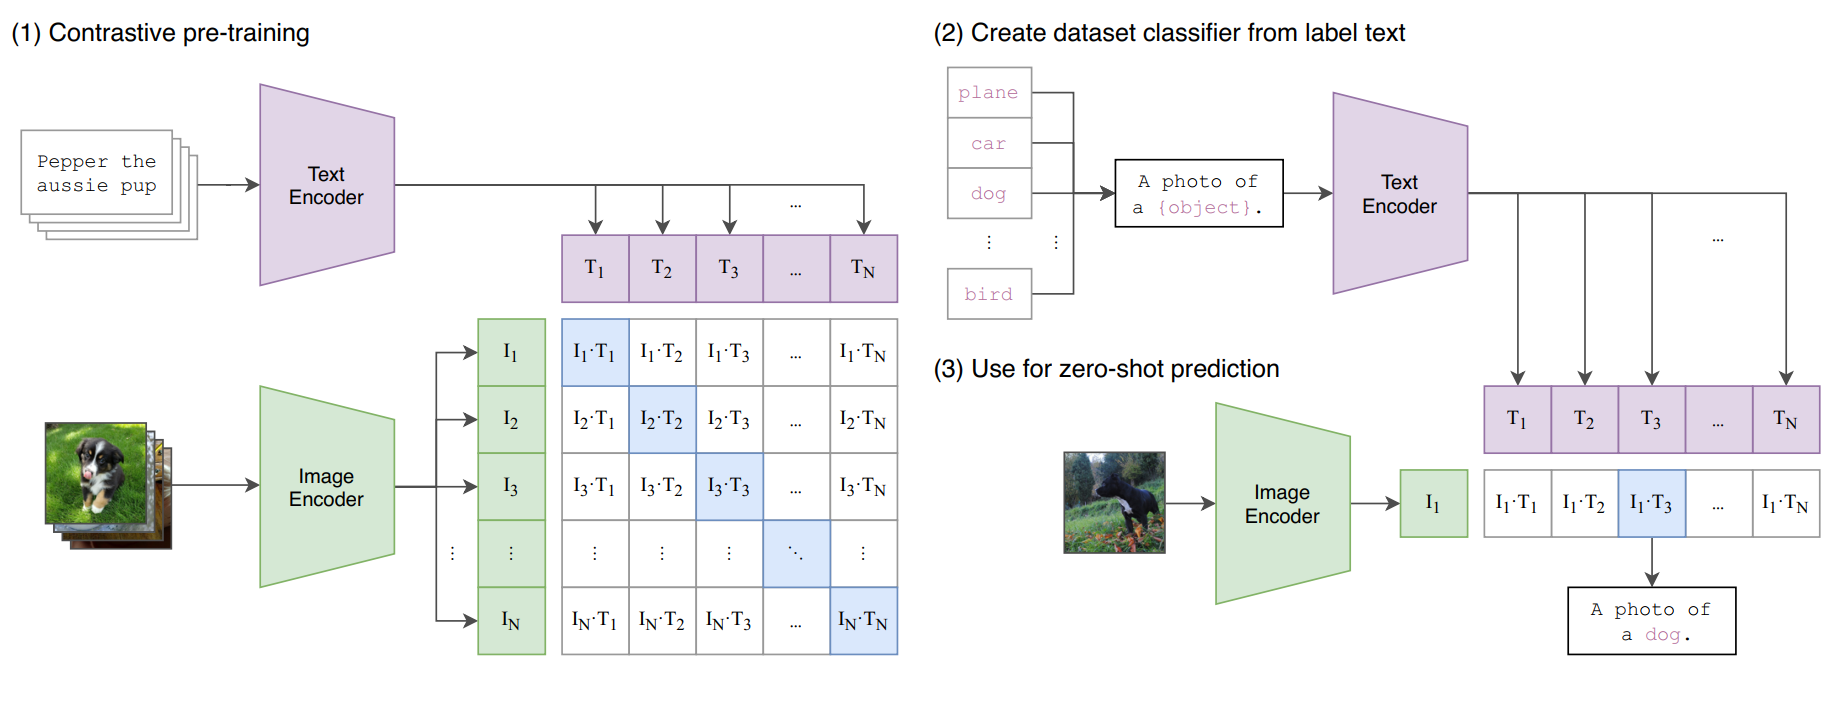
\includegraphics[width=0.95\textwidth]{../results/plots/methodology/clip_paradigm_radford2021.png}
    \caption{The CLIP paradigm as introduced by Radford et al., 2021 (Figure 1 of the original paper, reproduced for illustration). \textbf{(1) Contrastive pre-training}: two encoders project a batch of image--text pairs into a shared embedding space; the in-batch cosine-similarity matrix is supervised so the diagonal pairs (matched) score higher than off-diagonals (mismatched). \textbf{(2) Build a dataset-specific classifier from label text}: any new task is cast as text by encoding class-name prompts through the same text encoder. \textbf{(3) Zero-shot prediction}: an unseen image is classified by cosine-similarity argmax against the class prompts --- no task-specific training needed.}
    \label{fig:clip-paradigm}
\end{figure}

\begin{figure}[ht]
    \centering
    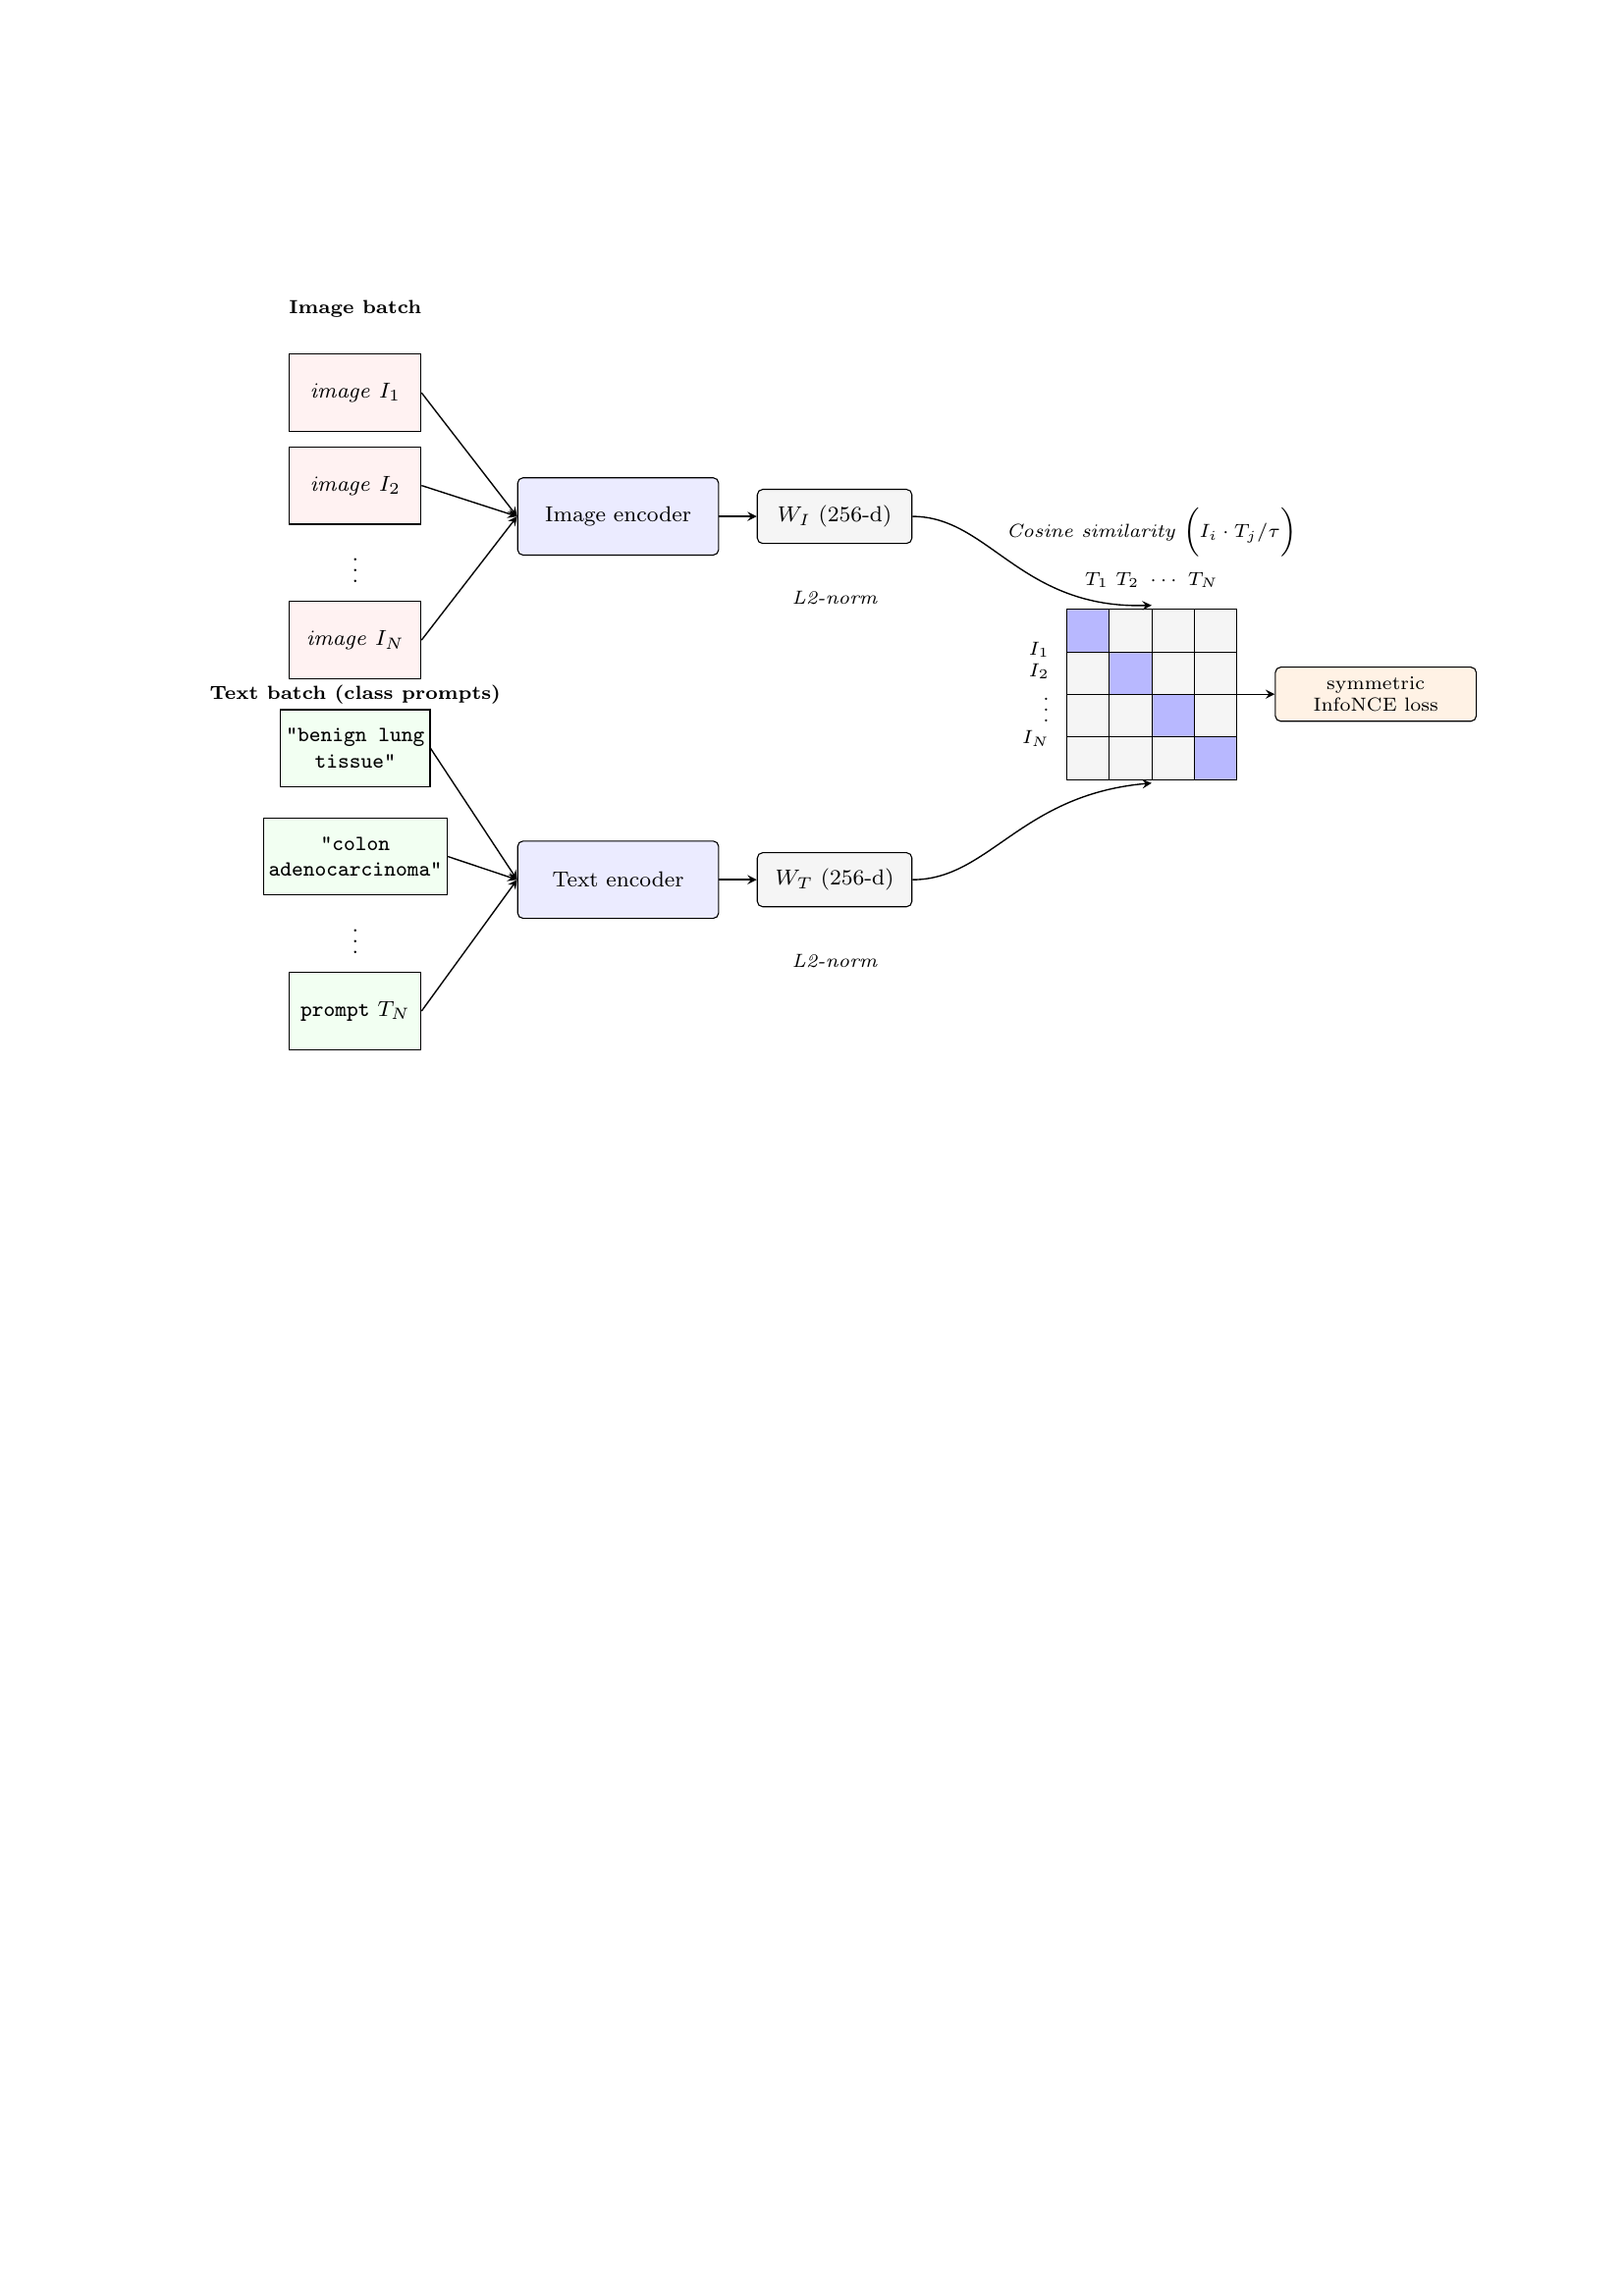
\begin{tikzpicture}[
        font=\footnotesize,
        x=1cm, y=1cm,
        encoder/.style ={draw, rounded corners=2pt, minimum width=2.6cm, minimum height=1.0cm,
                         fill=blue!8, line width=0.4pt},
        proj/.style    ={draw, rounded corners=2pt, minimum width=2.0cm, minimum height=0.7cm,
                         fill=gray!8, line width=0.4pt},
        sample/.style  ={draw, minimum width=1.7cm, minimum height=1.0cm, line width=0.4pt,
                         align=center, inner sep=2pt},
        emb/.style     ={draw, circle, minimum size=0.45cm, inner sep=0pt, line width=0.3pt},
        arr/.style     ={->, >=stealth, line width=0.5pt},
        >=stealth,
    ]
    %% Left -- inputs
    \node[sample, fill=red!5]  (img1) at (0,  1.6) {\textit{image} $I_1$};
    \node[sample, fill=red!5]  (img2) at (0,  0.4) {\textit{image} $I_2$};
    \node                       at (0, -0.6) {$\vdots$};
    \node[sample, fill=red!5]  (imgN) at (0, -1.6) {\textit{image} $I_N$};

    \node[sample, fill=green!5] (txt1) at (0, -3.0) {\texttt{"benign lung}\\\texttt{tissue"}};
    \node[sample, fill=green!5] (txt2) at (0, -4.4) {\texttt{"colon}\\\texttt{adenocarcinoma"}};
    \node                        at (0, -5.4) {$\vdots$};
    \node[sample, fill=green!5] (txtN) at (0, -6.4) {\texttt{prompt}~$T_N$};

    %% Encoders
    \node[encoder] (imenc) at (3.4,  0.0) {Image encoder};
    \node[encoder] (txenc) at (3.4, -4.7) {Text encoder};

    %% Projections
    \node[proj] (improj) at (6.2,  0.0) {$W_I$ (256-d)};
    \node[proj] (txproj) at (6.2, -4.7) {$W_T$ (256-d)};

    %% L2 / temperature
    \node[align=center, font=\scriptsize\itshape] at (6.2,  -1.05) {L2-norm};
    \node[align=center, font=\scriptsize\itshape] at (6.2,  -5.75) {L2-norm};

    %% Arrows: inputs -> encoder (fan-in to encoder's western edge)
    \foreach \src in {img1, img2, imgN}
        \draw[arr] (\src.east) -- (imenc.west);
    \foreach \src in {txt1, txt2, txtN}
        \draw[arr] (\src.east) -- (txenc.west);

    %% Encoders -> projections
    \draw[arr] (imenc) -- (improj);
    \draw[arr] (txenc) -- (txproj);

    %% Cosine similarity matrix
    \def\mx{9.2}      % left edge of matrix
    \def\my{-3.4}     % bottom edge of matrix
    \def\cs{0.55}     % cell size
    \pgfmathsetmacro{\mtop}{\my + 4*\cs}
    \pgfmathsetmacro{\mright}{\mx + 4*\cs}
    \foreach \i in {0,1,2,3} {
        \foreach \j in {0,1,2,3} {
            \pgfmathsetmacro{\cx}{\mx + \j*\cs}
            \pgfmathsetmacro{\cy}{\my + (3-\i)*\cs}
            \ifnum\i=\j
                \draw[fill=blue!28, line width=0.2pt] (\cx,\cy) rectangle ++(\cs,\cs);
            \else
                \draw[fill=gray!8,  line width=0.2pt] (\cx,\cy) rectangle ++(\cs,\cs);
            \fi
        }
    }
    %% Matrix labels
    \node[anchor=south, font=\scriptsize] at (\mx + 2*\cs, \mtop + 0.15) {$T_1\ T_2\ \cdots\ T_N$};
    \node[anchor=east,  font=\scriptsize, align=right]
        at (\mx - 0.10, \my + 2*\cs) {$I_1$\\$I_2$\\$\vdots$\\$I_N$};
    \node[anchor=south, font=\scriptsize\itshape] at (\mx + 2*\cs, \mtop + 0.55)
        {Cosine similarity $\bigl(I_i \cdot T_j / \tau\bigr)$};

    %% Projection -> matrix arrows
    \draw[arr] (improj.east) .. controls (8.2, 0) and (8.6, -1.2) .. (\mx + 2*\cs, \mtop + 0.05);
    \draw[arr] (txproj.east) .. controls (8.2, -4.7) and (8.6, -3.6) .. (\mx + 2*\cs, \my - 0.05);

    %% InfoNCE loss callout
    \node[draw, rounded corners=2pt, fill=orange!10, line width=0.4pt,
          minimum width=2.6cm, minimum height=0.7cm, align=center, font=\scriptsize]
          (loss) at (\mright + 1.8, \my + 2*\cs) {symmetric\\InfoNCE loss};
    \draw[arr] (\mright, \my + 2*\cs) -- (loss.west);

    %% Section labels
    \node[font=\scriptsize\bfseries, anchor=south] at (0,  2.45) {Image batch};
    \node[font=\scriptsize\bfseries, anchor=south] at (0, -2.55) {Text batch (class prompts)};

    \end{tikzpicture}
    \caption{CLIP dual-encoder architecture used in this project. Two independent encoders project a batch of $N$ image--text pairs into a shared $d$-dimensional embedding space (here $d = 256$, the projection head's output). After L2-normalisation and a learnable temperature $\tau$, the $N \times N$ cosine-similarity matrix between every image and every prompt is the input to the symmetric InfoNCE loss. The diagonal (blue) entries are the positive pairs; off-diagonal entries are negatives within the batch.}
    \label{fig:clip-architecture}
\end{figure}

\subsection{PLIP: a histopathology-pretrained CLIP-style model}
\label{sec:meth-plip-model}

PLIP~\cite{huang2023plip} (Huang et al., 2023) is a CLIP-style model pretrained on histopathology image--text pairs. Its training corpus is OpenPath, $\sim 208$k image--text pairs scraped from Twitter conversations among pathologists (using hashtags like \texttt{\#GIPath}, \texttt{\#PathTwitter}, etc.), supplemented with a filtered subset of LAION; the architecture is a CLIP ViT-B/32 vision encoder paired with a CLIP-style text encoder, both trained contrastively starting from CLIP's natural-image initialisation. Figure~\ref{fig:plip-openpath} illustrates the data pipeline: pathologist tweets become image--caption pairs that feed the contrastive training matrix, and over many training steps the image and matching-text embeddings get pulled together in the shared space.

\begin{figure}[H]
    \centering
    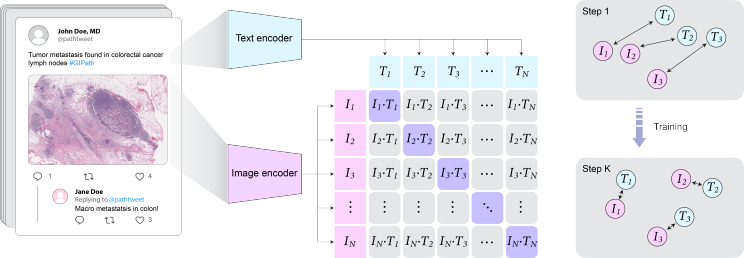
\includegraphics[width=0.95\textwidth]{../results/plots/methodology/external/plip_openpath_pipeline.png}
    \caption{The PLIP data pipeline and contrastive training. Left: a pathologist's Twitter post with an H\&E patch and a clinical description becomes an (image, text) training pair. Middle: PLIP's image and text encoders produce embeddings that are arranged into an $N \times N$ cosine-similarity matrix; the contrastive loss pulls the diagonal (matched) entries up and the off-diagonal entries down. Right: over many training steps, matched image--text pairs converge in the shared embedding space. Adapted from Huang et al.~\cite{huang2023plip}.}
    \label{fig:plip-openpath}
\end{figure}

\FloatBarrier

We use PLIP in two distinct ways. As a \emph{zero-shot reference baseline} (§\ref{sec:results-plip-zeroshot}), the full PLIP model --- image and text encoders both frozen --- is used off-the-shelf for cosine-similarity classification on all four datasets (LC25000 plus the three external evaluation sets). As a \emph{pretrained image encoder} in the image-encoder comparison (§\ref{sec:meth-image-vit}), only PLIP's ViT-B/32 vision encoder is used, paired with our LC25000-trained projection head and a separate BERT text encoder. The two roles isolate different questions: the first tests what pathology pretraining gives on its own; the second tests what pathology pretraining gives on top of LC25000 supervision.


\section{Image Encoders}
\label{sec:meth-image}

The image encoder is the component swapped in the central image-encoder comparison of this work (§\ref{sec:results-image-encoder}). Three encoders are compared: ResNet50 (§\ref{sec:meth-image-resnet}, the baseline's CNN, supervised on ImageNet); PLIP's ViT-B/32 (§\ref{sec:meth-image-vit}, the histopathology-contrastive ViT covered in §\ref{sec:meth-plip-model}); and DINOv2 ViT-B/14 (§\ref{sec:meth-image-dinov2}, general-domain self-supervised). The three were chosen to disentangle the three axes that change when ResNet50 is swapped for PLIP: the architecture (CNN vs ViT), the pretraining objective (supervised vs self-supervised vs contrastive), and the pretraining domain (natural images vs histopathology). DINOv2 specifically isolates ``ViT + self-supervision'' from ``histopathology pretraining'', acting as the control in the comparison.

A note on the following subsections: ResNet50 and DINOv2 below describe full encoder-plus-pretraining units, but the ViT subsection covers only the architecture --- the encoder we actually plug are PLIP's ViT-B/32 (already described in §\ref{sec:meth-plip-model}) and DINOv2's ViT-B/14. The two ViTs also differ in patch size (/32 vs /14), giving them different feature granularity at the same input resolution; this becomes a methodological caveat in the §\ref{sec:results-image-encoder} discussion.

\subsection{ResNet50 (CNN, ImageNet supervised)}
\label{sec:meth-image-resnet}

ResNet50~\cite{he2016resnet} (He et al., 2016) is the convolutional baseline. It is a deep residual network with $\sim 23$M parameters; the architecture's hallmark is the addition of skip connections that let gradients bypass groups of convolutional layers, which made it the first deep model that trained reliably at $50+$ layers. The output we use is the $2048$-d global-average-pooled feature vector from the final convolutional block. We use the standard ImageNet-1K supervised pretraining checkpoint ($\sim 1.3$M natural images, 1000 classes); no histopathology data is involved.

The role of ResNet50 in this work is as the general-purpose image-encoder baseline. Plugging it in as the image encoder carries the implicit assumption that ImageNet-supervised features transfer broadly enough to be useful on histopathology --- the assumption the encoder-swap comparison in §\ref{sec:results-image-encoder} tests directly.

\subsection{Vision Transformer (ViT)}
\label{sec:meth-image-vit}

The Vision Transformer~\cite{dosovitskiy2021vit} (ViT; Dosovitskiy et al., 2020) is the transformer architecture for images. Instead of convolution, the input image is split into a grid of fixed-size patches; each patch is linearly embedded as a token, and the resulting sequence is fed through a stack of transformer encoder layers with self-attention. The architecture has no built-in spatial bias of the kind a CNN's filters provide --- it learns spatial relationships from data, which is a large part of why ViTs need substantial pretraining to work well.

The variant we care about is ViT-Base (``B''), which has 12 transformer layers and a hidden size of 768. The suffix in names like ViT-B/16, ViT-B/32, ViT-B/14 denotes the patch size: a smaller patch means more tokens (finer spatial granularity) at the same input resolution. At our standard $224 \times 224$ input, ViT-B/32 produces $49$ patch tokens while ViT-B/14 produces $256$.

The role of this subsection is descriptive rather than operational: the actual image encoder we plug into the comparison is PLIP's pretrained ViT-B/32, already described in §\ref{sec:meth-plip-model}. The patch-size difference between PLIP's B/32 and DINOv2's B/14 is the methodological caveat previewed in the section intro and discussed in §\ref{sec:results-image-encoder}.

\subsection{DINOv2 (self-supervised on general natural images)}
\label{sec:meth-image-dinov2}

DINOv2~\cite{oquab2024dinov2} (Oquab et al., 2024) is a self-supervised Vision Transformer and the strongest general-purpose visual SSL backbone available at the time of writing, positioned by its authors as a default frozen feature extractor across a wide range of downstream vision tasks --- classification, segmentation, depth estimation, retrieval --- without task-specific fine-tuning. It builds on the original DINO~\cite{caron2021dino} framework (Caron et al., 2021), which introduced self-distillation for vision transformers, and scales it substantially: a larger curated training corpus, larger backbones, and a number of training-stability improvements.

The training corpus is LVD-142M, $\sim 142$M curated general natural images assembled by Meta from a $1.2$B raw image pool via retrieval-based curation; there are no class labels, no captions, and no histopathology data. The training signal is self-distillation: the model is split into a student and a teacher network with the same ViT architecture, and the student is trained to match the teacher's output on different augmented crops of the same image (Figure~\ref{fig:dino-framework}). The teacher is updated as an exponential moving average of the student's weights, so all supervision comes from the consistency of representations across augmentations --- no external labels are involved. The augmentation strategy is \emph{multi-crop}: the student sees both global crops (large, full-context views) and local crops (small, zoomed-in views) of the same image, while the teacher sees only the global crops. Notably, DINOv2 is \emph{not} a contrastive method --- there are no in-batch negatives and no InfoNCE loss; the consistency objective alone provides the supervision signal.

\begin{figure}[H]
    \centering
    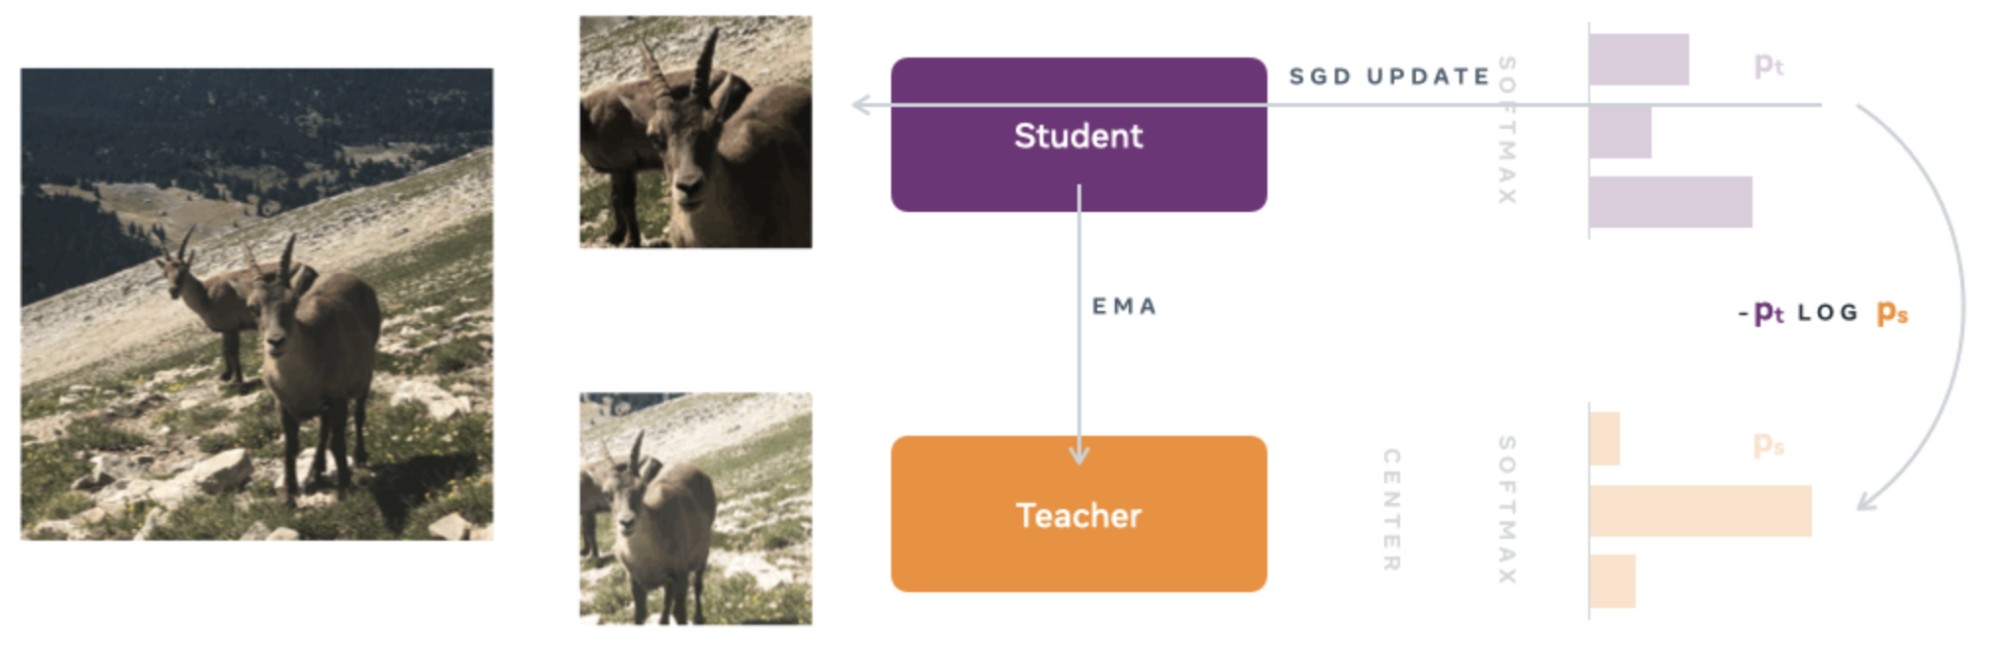
\includegraphics[width=0.85\textwidth]{../results/plots/methodology/external/dino_teacher_student.png}
    \caption{The DINO self-distillation framework used by DINOv2. Two augmented crops of the same image are fed through a student network and a teacher network; both produce softmax probability distributions $p_s$ and $p_t$. The student is trained via cross-entropy ($-p_t \log p_s$) to match the teacher's output and is updated by standard SGD; the teacher is updated as an exponential moving average (EMA) of the student's weights and is never directly trained. Adapted from Caron et al.~\cite{caron2021dino}.}
    \label{fig:dino-framework}
\end{figure}

\FloatBarrier

DINOv2 is released in four sizes (ViT-S/14, B/14, L/14, g/14, ranging from $\sim 22$M to $\sim 1.1$B parameters). We use ViT-B/14: the same Base architecture (12 layers, hidden 768) as PLIP's encoder, but with $14 \times 14$ patches rather than $32 \times 32$, giving the $256$ patch tokens noted above.

The role of DINOv2 in this work is as the control in the image-encoder comparison. It shares the architecture family (ViT) and the self-supervised paradigm with PLIP's vision encoder but never sees a histopathology image during pretraining. Plugging DINOv2 in as the image encoder therefore isolates ``ViT + general-domain self-supervision'' from ``histopathology pretraining specifically'': if DINOv2 closes the gap to PLIP, the win is largely architectural; if it does not, the win is specifically about histopathology pretraining.


\section{Text Encoders}
\label{sec:meth-text}

The text encoder is the second component swapped, in the text-encoder comparison of §\ref{sec:results-text-encoder}. Three encoders are compared, all from the BERT family~\cite{devlin2019bert} (Devlin et al., 2019), so the underlying architecture --- a 12-layer Transformer~\cite{vaswani2017attention} with 768-d hidden states and WordPiece tokenisation --- is the same across them; what differs is the corpus each encoder was pretrained on.

The baseline text encoder is \texttt{bert-base-uncased}, BERT trained on BookCorpus + English Wikipedia. The two biomedical variants are:

\begin{itemize}
    \item \textbf{BioBERT}~\cite{lee2020biobert} (Lee et al., 2020): a BERT-base checkpoint that starts from the BERT initialisation and is further pretrained on PubMed abstracts and PMC full-text articles, on top of the original BERT corpus.
    \item \textbf{PubMedBERT}~\cite{gu2021pubmedbert} (Gu et al., 2021): a BERT-base checkpoint pretrained \emph{from scratch} on PubMed abstracts and PMC, with a biomedical-vocabulary WordPiece tokeniser rather than the general-English one.
\end{itemize}

WordPiece tokenisation splits each input word into subword pieces drawn from a fixed vocabulary: rare or compound words decompose into multiple pieces (with a leading \texttt{\#\#} marking each continuation), while common words tokenise as a single piece. A special \texttt{[CLS]} token is prepended to every input and a \texttt{[SEP]} token closes it; the pooled embedding read out of the \texttt{[CLS]} position is what the projection head receives.

The vocabulary differs across the three encoders. BERT and BioBERT share the same general-English WordPiece vocabulary --- BioBERT inherits BERT's tokeniser and only continues pretraining on biomedical text. PubMedBERT trains a custom WordPiece vocabulary from scratch on PubMed and PMC text, so domain terms are far more likely to be single tokens. Table~\ref{tab:bert-tokenization} shows the resulting fragmentation for the baseline's composed prompt: BERT and BioBERT both split ``histopathology'' into four pieces and ``adenocarcinoma'' into four or five, while PubMedBERT keeps both as single tokens. This is a concrete reason a biomedical encoder could in principle help downstream classification --- the §\ref{sec:results-text-encoder} comparison tests whether the advantage translates into measurable F1 gains.

\begin{table}[H]
    \centering
    \small
    \begin{tabular}{|l|p{0.6\textwidth}|c|}
    \hline
    \textbf{Encoder} & \textbf{Tokens for ``A histopathology image of lung adenocarcinoma''} & \textbf{\#} \\ \hline
    BERT       & \texttt{[CLS] a his \#\#top \#\#ath \#\#ology image of lung aden \#\#oca \#\#rc \#\#ino \#\#ma [SEP]} & 15 \\ \hline
    BioBERT    & \texttt{[CLS] a his \#\#top \#\#ath \#\#ology image of lung ad \#\#eno \#\#car \#\#cin \#\#oma [SEP]} & 15 \\ \hline
    PubMedBERT & \texttt{[CLS] a histopathology image of lung adenocarcinoma [SEP]} & 8 \\ \hline
    \end{tabular}
    \caption{WordPiece tokenisation of the baseline composed prompt across the three text encoders. PubMedBERT's domain-trained vocabulary handles ``histopathology'' and ``adenocarcinoma'' as single tokens; BERT and BioBERT share BERT's general-English vocabulary, which fragments both terms into multiple wordpieces.}
    \label{tab:bert-tokenization}
\end{table}

All three encoders are dropped into the same baseline pipeline without other changes, isolating ``text-encoder pretraining'' as a single variable. The §\ref{sec:results-text-encoder} comparison crosses these three encoders with two prompt-format variants (bare class name vs ``A histopathology image of \{class\}.''), giving the 6-cell grid evaluated on NCT-CRC and extended to Chaoyang and LungHist700 for the best biomedical cell.


\section{Training Dataset: LC25000}
\label{sec:meth-dataset}

LC25000~\cite{borkowski2019lc25000} (Borkowski et al., 2019) is the only dataset used for training in this work. It contains five tissue classes spanning two organs --- benign lung tissue, lung adenocarcinoma, lung squamous cell carcinoma, benign colon tissue, and colon adenocarcinoma (Figure~\ref{fig:lc25000-samples}) --- with $5\,000$ patches per class for a total of $25\,000$ patches at $768 \times 768$ resolution. The patches are derived from $1\,250$ source images ($250$ per class) via geometric augmentation: each source is expanded into $20$ patches by random rotation and horizontal/vertical flipping; we do not add further augmentation on top. Table~\ref{tab:lc25000-splits} shows the stratified $80/10/10$ train/val/test split we use.

\textbf{Augmentation-pair leakage.} Because the $20$ augmented patches per source share image content, randomly splitting the $25\,000$ patches lets augmented copies of the same source image fall on both sides of the train/test split. We do not mitigate this in the runs reported here; it is flagged as a limitation in Chapter~\ref{chp:conclusion}. The leakage inflates in-distribution numbers --- every trained variant in this work saturates LC25000 at $\sim 0.99$ macro-F1 --- but does not affect the external-evaluation results that drive the chapter's conclusions, since no LC25000 source images appear in any external dataset.

The dataset has other known limits: it is a single-institution release, may contain stain artifacts, and lacks patient-level grouping or clinical validation. These are discussed in §\ref{sec:concl-limitations}.

\begin{figure}[H]
    \centering
    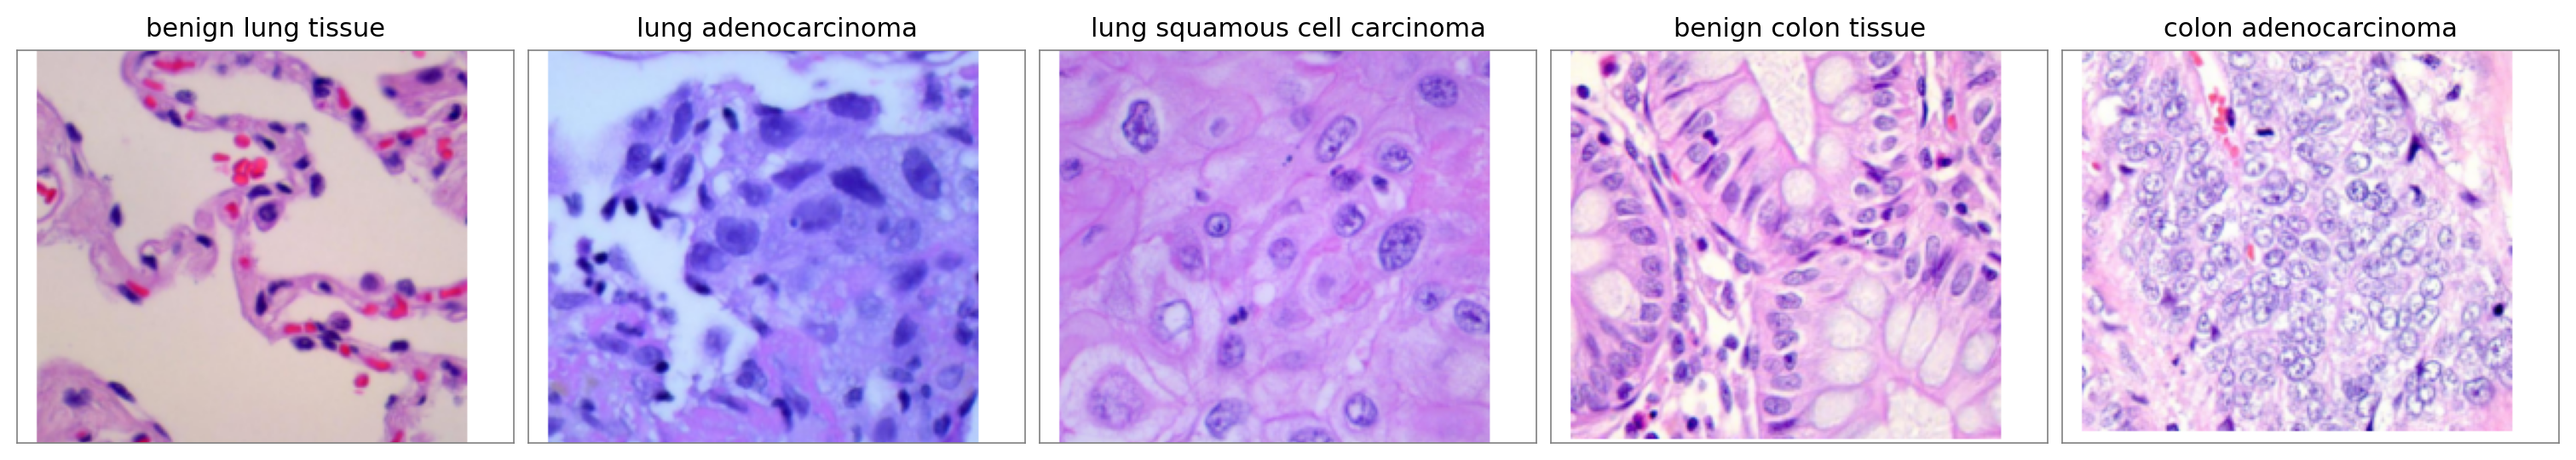
\includegraphics[width=0.95\textwidth]{../results/plots/methodology/lc25000_class_samples.png}
    \caption{Example image per class from LC25000. Left-to-right: benign lung tissue, lung adenocarcinoma, lung squamous cell carcinoma, benign colon tissue, colon adenocarcinoma. The two benign classes appear visually distinct from the cancer classes; within the cancers, lung adenocarcinoma vs lung squamous cell carcinoma is the hardest discrimination in our experiments (and a clinical confound).}
    \label{fig:lc25000-samples}
\end{figure}

\begin{table}[H]
    \centering
    \begin{tabular}{|l|c|c|c|c|}
    \hline
    \textbf{Class} & \textbf{Total} & \textbf{Train} & \textbf{Val} & \textbf{Test} \\ \hline
    benign lung tissue              & 5\,000 & 4\,000 & 500 & 500 \\ \hline
    lung adenocarcinoma             & 5\,000 & 4\,000 & 500 & 500 \\ \hline
    lung squamous cell carcinoma    & 5\,000 & 4\,000 & 500 & 500 \\ \hline
    benign colon tissue             & 5\,000 & 4\,000 & 500 & 500 \\ \hline
    colon adenocarcinoma            & 5\,000 & 4\,000 & 500 & 500 \\ \hline
    \textbf{Total}                  & 25\,000 & 20\,000 & 2\,500 & 2\,500 \\ \hline
    \end{tabular}
    \caption{LC25000 class counts and stratified split sizes.}
    \label{tab:lc25000-splits}
\end{table}

\FloatBarrier


\section{External Evaluation Datasets}
\label{sec:meth-external-datasets}

Each LC25000-trained variant is evaluated on three external datasets the model has never seen during training. The three are presented below in order of increasing shift severity relative to LC25000.

\subsection{NCT-CRC-HE-7K}

NCT-CRC-HE-7K~\cite{kather2019nct} (Kather et al., 2019; Zenodo record 1214456) is a colorectal-cancer patch dataset with $7\,180$ patches across 9 tissue classes. We restricted the evaluation to the (NORM $\leftrightarrow$ benign colon tissue) and (TUM $\leftrightarrow$ colon adenocarcinoma) classes that map to LC25000, giving $1\,974$ patches scored (741 NORM + 1\,233 TUM). The patches are $224 \times 224$ at $\sim 20\times$ magnification and arrive Macenko-normalised at release. NCT-CRC-HE-7K is the \textbf{close-shift colon} evaluation, stylistically similar to LC25000's colon side.

\subsection{Chaoyang}

Chaoyang~\cite{zhu2021chaoyang} (Zhu et al., 2022; preprint 2021) is a colorectal-cancer patch dataset from Beijing Chaoyang Hospital, $6\,160$ patches across 4 classes (normal, serrated, adenocarcinoma, adenoma). We restrict to normal ($\leftrightarrow$ benign colon, $n = 1\,816$) and adenocarcinoma ($\leftrightarrow$ colon adeno, $n = 2\,244$) for $4\,060$ patches scored. The patches are $512 \times 512$ at $20\times$, from a different hospital, scanner, and staining protocol than LC25000. The training split has documented label noise; the test split is labelled by consensus of three pathologists, and is the only split we use. Chaoyang is the \textbf{different-hospital colon} evaluation.

\subsection{LungHist700}

LungHist700~\cite{tabatabaei2024lunghist} (Tabatabaei et al., 2024, \emph{Scientific Data}) is a lung tissue dataset with $\sim 691$ high-resolution images at $20\times$ and $40\times$ magnifications, covering normal lung tissue plus adenocarcinoma and squamous-cell carcinoma at three differentiation grades each. We restrict to the $20\times$ subset for 3-class scoring: 359 images (85 normal, 146 adenocarcinoma, 128 squamous cell carcinoma). LungHist700 is the \textbf{different-source lung} evaluation, and the only multi-class external scoring in this work.


\section{Preprocessing and Input Pipeline}
\label{sec:meth-pre}

\subsection{Image preprocessing (per-backbone)}

Each image encoder expects pixel values in the distribution it was pretrained on, so the preprocessing we apply depends on which backbone we're using (Table~\ref{tab:image-preprocessing}). All inputs are resized to $224 \times 224$ with bilinear interpolation before they hit the encoder. We don't add any further augmentation on top: LC25000 already ships with rotation/flip augmentation at release, and the external evaluation sets are used as-is.

\begin{table}[H]
    \centering
    \small
    \begin{tabular}{|l|p{0.72\textwidth}|}
    \hline
    \textbf{Backbone} & \textbf{Preprocessing} \\ \hline
    ResNet50            & RGB / $255.0$ (i.e.\ $[0, 1]$ linear scaling) \\ \hline
    ViT-B/32 (PLIP)     & CLIP-standard mean/std normalisation: mean $=[0.481, 0.458, 0.408]$, std $=[0.269, 0.261, 0.276]$ \\ \hline
    ViT-B/14 (DINOv2)   & ImageNet mean/std normalisation: mean $=[0.485, 0.456, 0.406]$, std $=[0.229, 0.224, 0.225]$ \\ \hline
    \end{tabular}
    \caption{Per-backbone image preprocessing. Each backbone expects the input distribution it was pretrained on; mismatched preprocessing produces degraded features (see §\ref{sec:meth-preprocessing-bug}).}
    \label{tab:image-preprocessing}
\end{table}

\subsection{Text preprocessing}

All text encoders in this work use BERT-family WordPiece tokenisers (BERT, BioBERT, PubMedBERT, and PLIP's text encoder). We pad or truncate every input to a fixed sequence length of 24 tokens, which leaves comfortable headroom for every class-prompt format we test. The baseline's composed prompt template is \texttt{"A histopathology image of \{class\_name\}."}.

\subsection{LC25000-specific cleanup}

We apply two cleanup passes to LC25000 before training. First, we generate a canonical $80/10/10$ stratified train/val/test split with seed $42$ and check it into the repository as JSON, so every variant we train uses the exact same partition. Second, an MD5 pass over LC25000's files turns up $1\,280$ byte-identical duplicates, which we exclude via a dedupe-exclusion list (\texttt{src/data/lc25000\_dedupe\_exclusions.json}). One catch: the canonical split file pre-dates the dedupe pass, so the duplicates still cross the train/test boundary in the runs reported here. We flag this as a limitation in §\ref{sec:concl-limitations}.

\subsection{Methodological note on preprocessing}
\label{sec:meth-preprocessing-bug}

One bug worth recording surfaced mid-project. For a while, the pipeline was applying Caffe-style BGR mean-subtraction to a backbone that expected $[0, 1]$ RGB --- the mismatch came from two libraries shipping different ResNet50 checkpoints under the same name. The bug surfaced when a simple linear-probe diagnostic on the frozen features came back with a macro-F1 \emph{higher} than the trained CLIP ceiling, which should not happen. We fixed it by routing every image read through a centralised loader (\texttt{src/data/images.py}). The broader takeaway is methodological: linear-probing a frozen feature extractor against the trained model's ceiling is a cheap sanity check worth running early in any project.


\section{The Baseline}
\label{sec:meth-baseline}

The baseline pipeline is a frozen ResNet50 image encoder paired with a frozen BERT-base-uncased text encoder, with two small projection heads (\texttt{Dense(256, bias=False)} $\rightarrow$ \texttt{LayerNorm}) mapping each side into the shared $256$-d embedding space. Only the projection heads and the learnable temperature $\tau$ (initialised at $0.07$ following CLIP) are trained. The loss is symmetric InfoNCE, optimised with AdamW and gradient clipping; the same composed prompt template is used at training and at inference. All computation runs in float32. Table~\ref{tab:baseline-hyperparameters} gives the full hyperparameter list. Each variant in the experiment matrix changes exactly one row of this table; everything else is held constant.

\begin{table}[H]
    \centering
    \begin{tabular}{|l|l|}
    \hline
    \textbf{Hyperparameter} & \textbf{Value} \\ \hline
    Image encoder              & ResNet50 (ImageNet preset), frozen \\ \hline
    Text encoder               & BERT base uncased, frozen \\ \hline
    Projection head            & Dense(256, no bias) $\to$ LayerNorm \\ \hline
    Embedding dimension        & 256 \\ \hline
    Image size                 & $224 \times 224$ \\ \hline
    Text sequence length       & 24 WordPiece tokens \\ \hline
    Batch size                 & 32 \\ \hline
    Initial temperature        & $\tau = 0.07$ \\ \hline
    Loss                       & symmetric InfoNCE \\ \hline
    Optimizer                  & AdamW \\ \hline
    Learning rate              & $1 \times 10^{-3}$ \\ \hline
    Weight decay               & $1 \times 10^{-4}$ \\ \hline
    Gradient clipnorm          & 1.0 \\ \hline
    Max epochs                 & 30 \\ \hline
    EarlyStopping patience     & 5 \\ \hline
    ReduceLROnPlateau          & factor 0.5, patience 2, min $10^{-6}$ \\ \hline
    Numerical precision        & float32 \\ \hline
    Random seed                & 42 \\ \hline
    \end{tabular}
    \caption{Baseline hyperparameters. Each variant in the experiment matrix changes exactly one row.}
    \label{tab:baseline-hyperparameters}
\end{table}

\FloatBarrier


\section{Evaluation Protocol}
\label{sec:meth-eval}

\subsection{Metrics and visualizations}

We use two classification rules, depending on the variant. CLIP variants predict by taking the argmax of cosine similarity between the image embedding and the five LC25000 class-prompt embeddings; the plain classifier (§\ref{sec:results-foundational-vs-plain}) predicts by taking the argmax of the softmax over its \texttt{Dense(5)} output. All the metrics reported in the Results chapter follow from one of these two rules.

The global metrics reported throughout this work are:
\begin{itemize}
    \item \textbf{Accuracy} --- the fraction of samples whose predicted class matches the true class:
    $$\text{Accuracy} = \frac{1}{N} \sum_{i=1}^{N} \mathbb{1}[\hat{y}_i = y_i].$$
    \item \textbf{Balanced accuracy} --- the macro-average of per-class recall: equal weight to every class regardless of its support, so a single-class predictor on an imbalanced dataset cannot game the metric:
    $$\text{Balanced Accuracy} = \frac{1}{K} \sum_{k=1}^{K} R_k, \qquad R_k = \frac{\mathrm{TP}_k}{\mathrm{TP}_k + \mathrm{FN}_k}.$$
    \item \textbf{Macro-F1} --- the macro-average of per-class F1 (harmonic mean of precision and recall), again with equal weight per class. This is the headline metric throughout, chosen because external evaluations have imbalanced class supports and macro-F1 penalises class collapse symmetrically:
    $$\text{Macro-F1} = \frac{1}{K} \sum_{k=1}^{K} F1_k, \qquad F1_k = \frac{2 \, P_k R_k}{P_k + R_k}.$$
    \item \textbf{Weighted F1} --- per-class F1 weighted by class support; emphasises majority classes. Reported alongside macro-F1 for completeness:
    $$\text{Weighted F1} = \sum_{k=1}^{K} \frac{n_k}{N} \cdot F1_k.$$
\end{itemize}

We additionally report per-class precision, recall, F1, and support for every variant, along with confusion matrices (both raw counts and row-normalised by true class). For visualisations we produce a shared image-and-prompt UMAP on the training source (LC25000 test split), one fit per variant with points colour-coded by class; and a cross-distribution UMAP grid per external dataset where LC25000 image embeddings (circles, by class) are overlaid with external-dataset embeddings (triangles, by class) in a single shared UMAP fit per external dataset. All UMAPs use \texttt{umap-learn} with $n\_\text{neighbors}=15$, $\text{min\_dist}=0.1$, and cosine distance, fit on the L2-normalised projection-head output.

\subsection{External-dataset evaluation: restricted-argmax protocol}

External datasets cover only a subset of LC25000's classes --- NCT-CRC and Chaoyang are colon-only, LungHist700 is lung-only --- so an unrestricted argmax over all five LC25000 prompts would routinely predict the model's strongest out-of-organ class on these images and produce uninformative misclassifications. To avoid this, on external evaluation we restrict the argmax to the LC25000 classes that map to the external dataset's organ:

\begin{itemize}
    \item NCT-CRC and Chaoyang (colon datasets): argmax over \{benign colon tissue, colon adenocarcinoma\}.
    \item LungHist700 (lung dataset): argmax over \{benign lung tissue, lung adenocarcinoma, lung squamous cell carcinoma\}.
\end{itemize}

The full class-mapping rules per dataset are detailed in §\ref{sec:meth-external-datasets}. All external evaluation is pure inference: every variant reuses its LC25000-trained checkpoint with no fine-tuning on the external sets.

\subsection{Per-organ reporting}

Results in this work are reported per external dataset, never averaged across them. Averaging would hide the cross-organ regime change we see in Chapter~\ref{chp:results}: a single number across all external datasets would collapse the order-of-magnitude difference between the colon and lung sides into one misleading point. Reporting per-dataset is therefore an explicit choice driven by what the experiments showed, not the convenient default.


\section{Computational Setup and Reproducibility}
\label{sec:meth-compute}

All training and evaluation runs in this work were carried out on Google Colab (T4 GPU instances, occasionally L4 for the longer runs), with a local CPU/GPU fallback used for development and analysis. The main software stack is TensorFlow with KerasHub, which handles the CLIP-style training pipeline and every downstream evaluation. An auxiliary PyTorch + HuggingFace \texttt{transformers} stack is used only for image-encoder feature extraction when an encoder lacks a TensorFlow port (DINOv2, discussed below). Library versions are pinned in \texttt{requirements.txt} so the environment can be reproduced exactly.

Reproducibility is set up at three layers: a fixed random seed of $42$ across NumPy, TensorFlow, and PyTorch; \texttt{PYTHONHASHSEED} set explicitly; and \texttt{tf.config.experimental.enable\_op\_determinism()} called at the start of each run. Under these settings, repeat runs on the same hardware are bit-exact. Small numerical drift can appear across GPU types (T4 vs L4) due to floating-point ordering inside CUDA kernels, but it does not change the classification outcomes reported.

One practical caveat: DINOv2 has no TensorFlow port in our environment, so its image features are precomputed once in PyTorch and cached to disk as HDF5 files (one per dataset, keyed by image relative path). The TensorFlow training and evaluation pipelines then read from cache. This is mathematically equivalent to running the frozen backbone online --- the backbone is frozen, so every image always produces the same feature vector --- and it avoids the cost of running DINOv2 inference at every training step. The total cache footprint is $\sim 100$~MB across LC25000 and the three external datasets.


%Chapter 4: Results and Discussion
% !TEX root =../tfmETSI.tex
\chapter{Results and Discussion}\label{results}

% =====================================================================
%  Pass D (2026-06-07) -- second review pass folding in the user's
%  comments on Pass C+ (sections 1-15 of the consolidated fix list,
%  numbered Q1-Q7 for the open questions resolved before this rewrite).
%
%  Structure: 8 sections (Limitations moved to chapter 5; Summary table
%  folded into Discussion as 4.8.5).
%   1. Experimental Overview
%   2. Baseline
%   3. Stain normalization        (moved here -- input-side axis)
%   4. PLIP zero-shot reference
%   5. Foundational model vs plain classifier
%   6. Text encoder pretraining
%   7. Image encoder pretraining (HEADLINE)
%   8. Discussion
%
%  Per-section template (default; may collapse where uninformative):
%     Configuration -> Training source results -> Generalization to
%     external datasets -> What we learned
% =====================================================================

\providecommand{\stale}[1]{{\color{orange}#1\textsuperscript{\dag}}}
\providecommand{\todo}[1]{\textcolor{orange}{\textit{[TODO: #1]}}}
\providecommand{\pending}[1]{\textcolor{blue}{\textit{[pending: #1]}}}

% ============================================================
\section{Experimental Overview}
\label{sec:results-overview}

\subsection{Research questions}
\label{sec:results-rqs}

The chapter is built around six research questions, each targeting a single design axis of a CLIP-style histopathology pipeline: the baseline reference, the CLIP-versus-non-CLIP choice, the input-side preprocessing, the text encoder, the image encoder, and cross-dataset generalisation. Five of them (RQ1--RQ5) are answered by a dedicated experiment section in this chapter; RQ6 is cross-cutting and is addressed by the external evaluations run alongside every other experiment. The experiment matrix in Table~\ref{tab:experiment-matrix} below maps each RQ to the controlled comparison that addresses it.

\begin{itemize}
    \item \textbf{RQ1} --- What baseline classification and generalisation behaviour does a frozen general-purpose CLIP pipeline achieve on LC25000, and what failure modes appear?
    \item \textbf{RQ2} --- Does the CLIP paradigm validate its \emph{foundational-model} premise --- learning one task and generalising to tasks it was not specifically trained for --- relative to a non-CLIP classifier on the same image encoder?
    \item \textbf{RQ3} --- Does stain normalisation, an input-side preprocessing that targets a known shortcut in histopathology, help when evaluating on datasets the model was never trained on?
    \item \textbf{RQ4} --- Does using a text encoder pretrained on biomedical text (BioBERT, PubMedBERT), instead of generic BERT, improve performance under short class-name prompts?
    \item \textbf{RQ5} --- Does the image encoder's \emph{pretraining choice} matter? We test two alternatives to the ImageNet-supervised ResNet50 baseline: (a) a Visual Transformer pretrained on histopathology image--text pairs (PLIP), and (b) a Visual Transformer pretrained self-supervised on general natural images (DINOv2), which serves as a control to separate the contribution of ``ViT architecture and self-supervision'' from ``histopathology pretraining specifically''.
    \item \textbf{RQ6} --- How well does each variant generalise to data the model has never seen? We evaluate every variant against three external datasets across two organs that span shift severity: close-shift colon, different-hospital colon, and different-source lung.
\end{itemize}

\begin{table}[ht]
\centering
\small
\newcolumntype{L}[1]{>{\raggedright\arraybackslash}p{#1}}
\footnotesize
\begin{tabular}{|L{2.0cm}|L{2.4cm}|L{2.2cm}|L{1.5cm}|L{1.9cm}|L{1.9cm}|}
\hline
\textbf{Experiment} & \textbf{Image encoder} & \textbf{Text encoder} & \textbf{Loss} & \textbf{Preprocessing} & \textbf{Axis tested} \\ \hline
Baseline (\S\ref{sec:results-baseline}) & ResNet50 (ImageNet) & BERT base & InfoNCE & RGB / 255 & reference \\ \hline
Stain normalization (\S\ref{sec:results-stain}) & ResNet50 (ImageNet) & BERT base & InfoNCE & Macenko / Reinhard / Vahadane & input-side \\ \hline
PLIP zero-shot (\S\ref{sec:results-plip-zeroshot}) & ViT-B/32 (PLIP / OpenPath) & PLIP text encoder & none (zero-shot) & CLIP mean/std & reference: no LC25000 supervision \\ \hline
Foundational vs plain (\S\ref{sec:results-foundational-vs-plain}) & ResNet50 (ImageNet) & --- (no text) & cross-entropy & RGB / 255 & architecture: CLIP paradigm vs plain classifier \\ \hline
Text encoder (\S\ref{sec:results-text-encoder}) & ResNet50 (ImageNet) & BioBERT / PubMedBERT & InfoNCE & RGB / 255 & text encoder pretraining \\ \hline
Image encoder (\S\ref{sec:results-image-encoder}) & ViT-B/32 (PLIP); ViT-B/14 (DINOv2) & BERT base & InfoNCE & varies & image encoder pretraining \\ \hline
\end{tabular}
\caption{Experiment matrix. Each experiment isolates exactly one axis of variation relative to the baseline. Sections \S\ref{sec:results-baseline}--\S\ref{sec:results-image-encoder} follow this order, ending with image-encoder pretraining (the chapter's headline finding).}
\label{tab:experiment-matrix}
\end{table}

\subsection{Training source and external datasets}
\label{sec:results-ood-framework}

Every variant in this chapter is trained on a single source dataset and evaluated on three external datasets it has never seen during training. The training source is LC25000~\cite{borkowski2019lc25000}, already introduced in §\ref{sec:results-baseline-config}: every trained variant is fit on it, and the in-distribution test split yields the macro-F1 we refer to as \emph{training-source results} throughout the chapter. The three external datasets --- the source of every \emph{generalisation} number in the chapter --- are listed in order of shift severity:

\begin{itemize}
    \item \textbf{NCT-CRC-HE-7K}~\cite{kather2019nct}, close-shift colon: $1\,974$ scored patches over the \texttt{NORM} and \texttt{TUM} classes, mapping to \emph{benign colon tissue} and \emph{colon adenocarcinoma} in LC25000.
    \item \textbf{Chaoyang}~\cite{zhu2021chaoyang}, different-hospital colon: $4\,060$ scored patches (\texttt{normal} and \texttt{adenocarcinoma}; the \texttt{serrated} and \texttt{adenoma} classes have no clean LC25000 analogue and are excluded from scoring), mapping to the same two LC25000 colon classes as NCT.
    \item \textbf{LungHist700}~\cite{tabatabaei2024lunghist}, different-source lung: $359$ images at $20\times$ magnification (the $40\times$ subset is excluded), mapping to LC25000's \emph{benign lung tissue}, \emph{lung adenocarcinoma}, and \emph{lung squamous cell carcinoma}.
\end{itemize}

Full dataset provenance, acquisition details, and per-dataset preprocessing live in Methodology (§\ref{sec:meth-external-datasets}); the bullets above keep only what is needed to interpret the external-evaluation tables in the rest of the chapter.

Three protocol choices apply to every external evaluation that follows. First, \textbf{restricted argmax}: each variant exposes all $5$ LC25000 class prompts at inference, but the argmax is restricted to the LC25000 classes that map to the external dataset's organ ($2$ colon classes for NCT and Chaoyang, $3$ lung classes for LungHist700). Predictions into a non-target LC25000 class count as wrong but are reported separately when informative for confusion analysis. Second, \textbf{pure inference}: every variant reuses its LC25000-trained checkpoint without further adaptation; no fine-tuning is performed on the external datasets. Third, \textbf{per-dataset reporting}: results are presented per dataset rather than averaged. The motivation for that last choice is methodological --- aggregating across datasets would average a colon-side partial transfer ($\sim 0.79$--$0.87$ F1) with a lung-side categorical failure ($0.305$ F1 in the baseline), producing a single mean-OOD number that hides the cross-organ regime change that ends up driving the chapter's headline result in §\ref{sec:results-image-encoder}.

\subsection{Metrics and visualizations}
\label{sec:results-metrics}

Each variant in this chapter is reported with the same set of metrics and visualisations. The choices and what each is meant to surface:
\begin{itemize}
    \item \textbf{Macro-F1} is the headline metric. It averages the per-class F1 scores equally, which is the right behaviour for the per-class precision--recall trade-offs that drive the chapter's substantive comparisons. Formal definitions are in Methodology (§\ref{sec:meth-eval}).
    \item \textbf{Accuracy, balanced accuracy, weighted F1, and per-class precision/recall/F1} are reported alongside macro-F1 for completeness, but the chapter's interpretive weight is on macro-F1 and the per-class numbers.
    \item \textbf{Confusion matrices} (raw counts and row-normalised by true class) are reported per variant and per dataset --- the most direct view of how a model distributes its errors across the available classes.
    \item \textbf{Training-source UMAP} projects LC25000 image embeddings and class-prompt embeddings into the same 2-D fit (cosine metric), letting the reader see cluster separation and the alignment between image clusters and prompt anchors.
    \item \textbf{Cross-distribution UMAP grid} (per external dataset, per variant) overlays LC25000 dots and external-dataset triangles in a single 2-D fit, asking whether the external dataset co-locates with the matching LC25000 class cluster or sits in its own region of feature space.
\end{itemize}


% ============================================================
\section{Baseline: frozen ResNet50 and frozen BERT}
\label{sec:results-baseline}

\subsection{Configuration}
\label{sec:results-baseline-config}

The baseline pipeline pairs a frozen ResNet50 image encoder, taken from the standard ImageNet-supervised checkpoint, with a frozen BERT-base-uncased text encoder; only a pair of small projection heads --- a single $256$-wide \texttt{Dense} layer with no bias, followed by \texttt{LayerNorm} --- and a scalar temperature $\tau$ are trained on top. This is deliberately the most general-purpose CLIP one can assemble. ResNet50 is the canonical CNN baseline of the past decade and BERT-base is the canonical text encoder; neither has been exposed to histology during pretraining, and neither has been tuned for the task. The reason to start here is mechanical: every subsequent variant in this chapter changes exactly one piece of this configuration, and the resulting delta is only interpretable if the reference is something recognisable rather than something already adapted to the data.

Everything else is held constant across the variants that follow. The training data is the LC25000 dataset, with a $80/10/10$ train--validation--test split at random seed $42$; a single fixed composed prompt, \texttt{``A histopathology image of \{class\_name\}.''}, is used at both training and inference; the loss is symmetric InfoNCE; the optimiser is AdamW with learning rate $1 \times 10^{-3}$ and weight decay $1 \times 10^{-4}$; and training runs for at most $30$ epochs, with EarlyStopping (patience $5$, restore best weights) terminating it earlier on every run. The remaining design choices --- batch size, image and sequence dimensions, initial temperature, gradient clipping, learning-rate schedule, numerical precision, weight initialisation --- are not referenced again in this chapter and are gathered in the baseline hyperparameter table in Methodology (Table~\ref{tab:baseline-hyperparameters}).

\subsection{Training behaviour and in-distribution results}
\label{sec:results-baseline-training}

On the LC25000 test split, the baseline reaches a macro-F1 of $0.996$. The model has only two trainable projection heads and a scalar temperature $\tau$ on top of frozen encoders --- around $720{,}000$ parameters in total --- so a saturated in-distribution score would invite a memorisation reading without a check on the training dynamics. Figure~\ref{fig:baseline-loss} provides that check: the training and validation InfoNCE losses (equation~\eqref{eq:infonce-sym}) descend together over the $30$-epoch budget and stay close at convergence. The learnable temperature $\tau$ (equation~\eqref{eq:scaled-cosine}), initialised at the CLIP-paper value of $0.07$, \emph{rises} during training, peaks at $\approx 0.090$ around epoch $10$, and settles near $0.087$. This is the opposite direction from the CLIP paper's $\tau \to 0.01$ behaviour on uniquely-paired image--text data, and is consistent with our shared-prompt setup: when multiple images per batch share the same class prompt (the false-negative caveat in §\ref{sec:meth-clip}), softening $\tau$ reduces the penalty those false negatives impose on otherwise-correct alignments.

\begin{figure}[H]
    \centering
    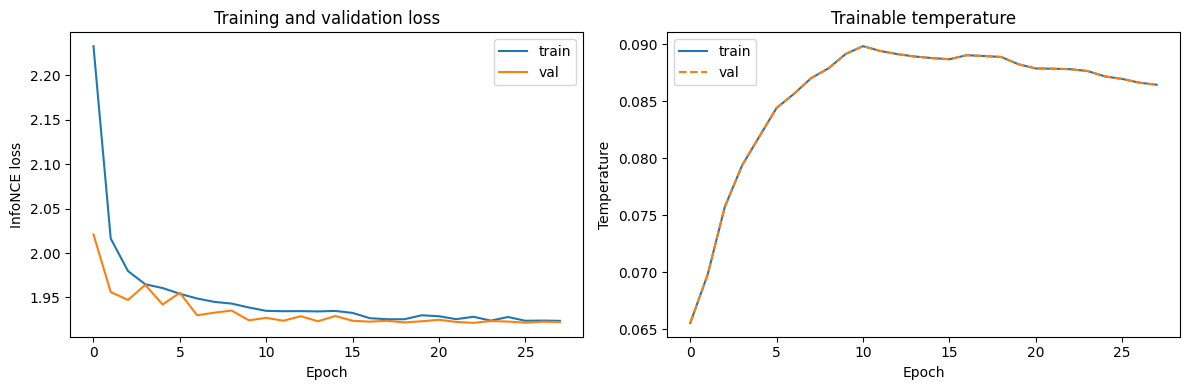
\includegraphics[width=0.9\textwidth]{../results/plots/baseline_loss.png}
    \caption{Baseline training (blue) and validation (orange) InfoNCE loss across epochs (left), and the learnable temperature $\tau$ on the same horizontal axis (right).}
    \label{fig:baseline-loss}
\end{figure}

The embedding space the model converges to is shown in Figure~\ref{fig:baseline-umap}. Each LC25000 class forms a distinct cluster of image embeddings and the five class-prompt anchors (encoded through frozen BERT and projected to the same $256$-d space) sit at the centre of their corresponding clusters --- the expected post-InfoNCE alignment between text and image, with the trained projection heads doing the work that the frozen text encoder alone could not. The lung-adenocarcinoma cluster sits closest to lung squamous cell carcinoma in the 2D projection, foreshadowing the off-diagonal confusion-matrix mass discussed below.

\begin{figure}[H]
    \centering
    \begin{minipage}[t]{0.48\textwidth}
        \centering
        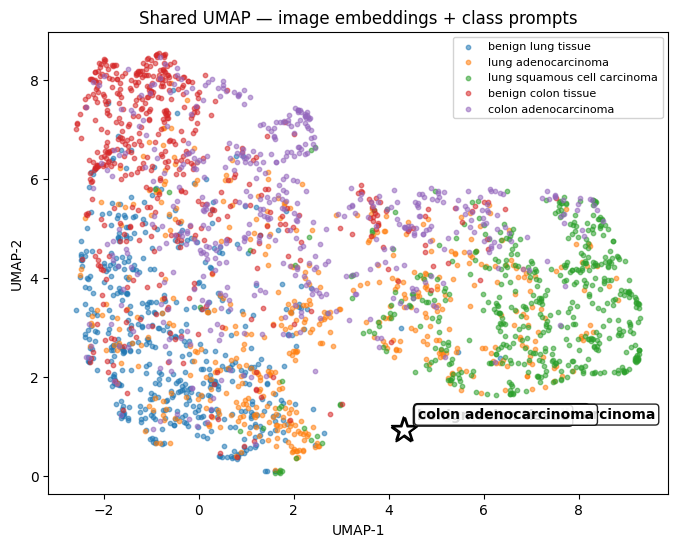
\includegraphics[width=\textwidth]{../results/plots/baseline_umap.png}
        \par\vspace{2pt}\footnotesize (a) Vanilla scatter.
    \end{minipage}\hfill
    \begin{minipage}[t]{0.48\textwidth}
        \centering
        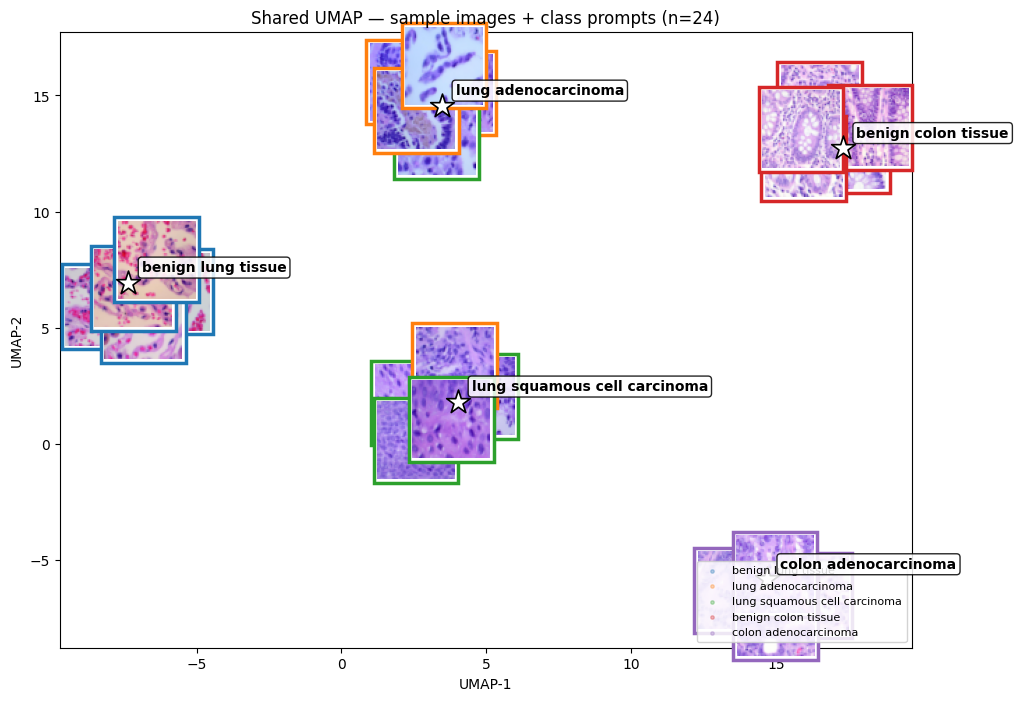
\includegraphics[width=\textwidth]{../results/plots/baseline_umap_thumbnails.png}
        \par\vspace{2pt}\footnotesize (b) Sample-image thumbnails.
    \end{minipage}
    \caption{UMAP of the baseline embedding space on the LC25000 test split. Two views of the same fit: (a) per-class scatter with the five class-prompt anchors marked, (b) the same fit overlaid with sample-image thumbnails.}
    \label{fig:baseline-umap}
\end{figure}

The confusion matrix (Figure~\ref{fig:baseline-cm}) confirms that the saturated $0.996$ is genuinely close to ceiling: the benign tissues and lung squamous cell carcinoma separate cleanly, with the off-diagonal mass concentrated on lung adenocarcinoma --- the hardest discrimination in the LC25000 schema. In-distribution, thus, does not discriminate the baseline from any of the trained variants studied in subsequent sections (all of them saturate at $\sim 0.99$); the meaningful comparison is the external evaluation that follows in §\ref{sec:results-baseline-ood}.

\begin{figure}[H]
    \centering
    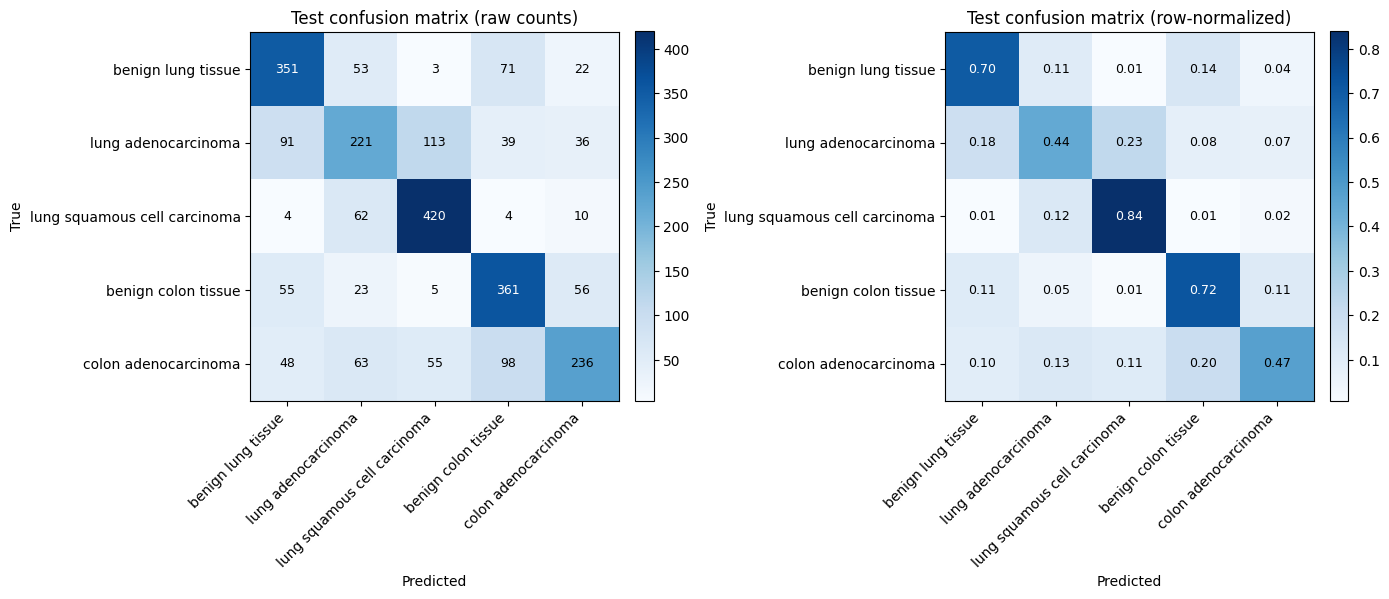
\includegraphics[width=0.95\textwidth]{../results/confusion_matrices/baseline_confusion_matrices.png}
    \caption{Baseline confusion matrix on the LC25000 test split. Left: raw counts. Right: row-normalised by true class.}
    \label{fig:baseline-cm}
\end{figure}

\FloatBarrier
\subsection{Generalization to external datasets}
\label{sec:results-baseline-ood}

The baseline's macro-F1 on each external dataset, restricted-argmax over the target-organ LC25000 classes, is reported in Table~\ref{tab:baseline-ood}. The result splits in two. On the two colon datasets the baseline transfers partially --- $0.866$ on NCT-CRC-HE-7K, the dataset stylistically closest to LC25000's colon distribution, and $0.786$ on Chaoyang, where a different hospital, scanner, and staining protocol drag the score down by $\sim 0.08$ F1 even though the organ is unchanged. On lung the picture is qualitatively different: \textbf{$\mathbf{0.305}$ macro-F1 on LungHist700's 3-class problem, where chance is $\mathbf{0.33}$}. The colon-versus-lung gap dwarfs every within-organ shift in the table --- the central observation the rest of the chapter sets out to explain.

\begin{table}[H]
    \centering
    \small
    \begin{tabular}{|l|c|c|c|c|}
    \hline
    \textbf{External dataset (organ)} & \textbf{Macro-F1} & \textbf{Accuracy} & \textbf{Bal.\ acc.} & \textbf{Weighted F1} \\ \hline
    NCT-CRC-HE-7K (colon)            & \textbf{0.866} & 0.870 & 0.866 & 0.871 \\ \hline
    Chaoyang (colon)                 & \textbf{0.786} & 0.796 & 0.782 & 0.791 \\ \hline
    LungHist700 (lung, 20$\times$)   & \textbf{0.305} & 0.390 & 0.383 & 0.301 \\ \hline
    \end{tabular}
    \caption{Baseline generalization to the three external datasets, restricted-argmax over the target-organ LC25000 classes.}
    \label{tab:baseline-ood}
\end{table}

The lung results are not a noisy degradation of the colon transfer; they are a different failure mode. Per-class recall on LungHist700 breaks down as $0.89$ for lung squamous cell carcinoma, $0.07$ for lung adenocarcinoma, and $0.19$ for benign lung tissue. Back-calculated from the precision figures, \textbf{the model assigns ``squamous'' to roughly $\mathbf{84}$\% of LungHist700 inputs regardless of true class} --- and given that squamous accounts for only $36$\% of the ground truth, the near-chance macro-F1 is the direct consequence of that bias. Figure~\ref{fig:baseline-lung-umap} shows the matching feature-space signature: all $359$ LungHist700 samples collapse into a single tight cluster with no visible internal class structure. The frozen ImageNet-supervised ResNet50, never exposed to histology during pretraining, extracts no usable per-class variance from LungHist700 tissue, and the trained projection head has nothing to align with the three lung class prompts.

\begin{figure}[H]
    \centering
    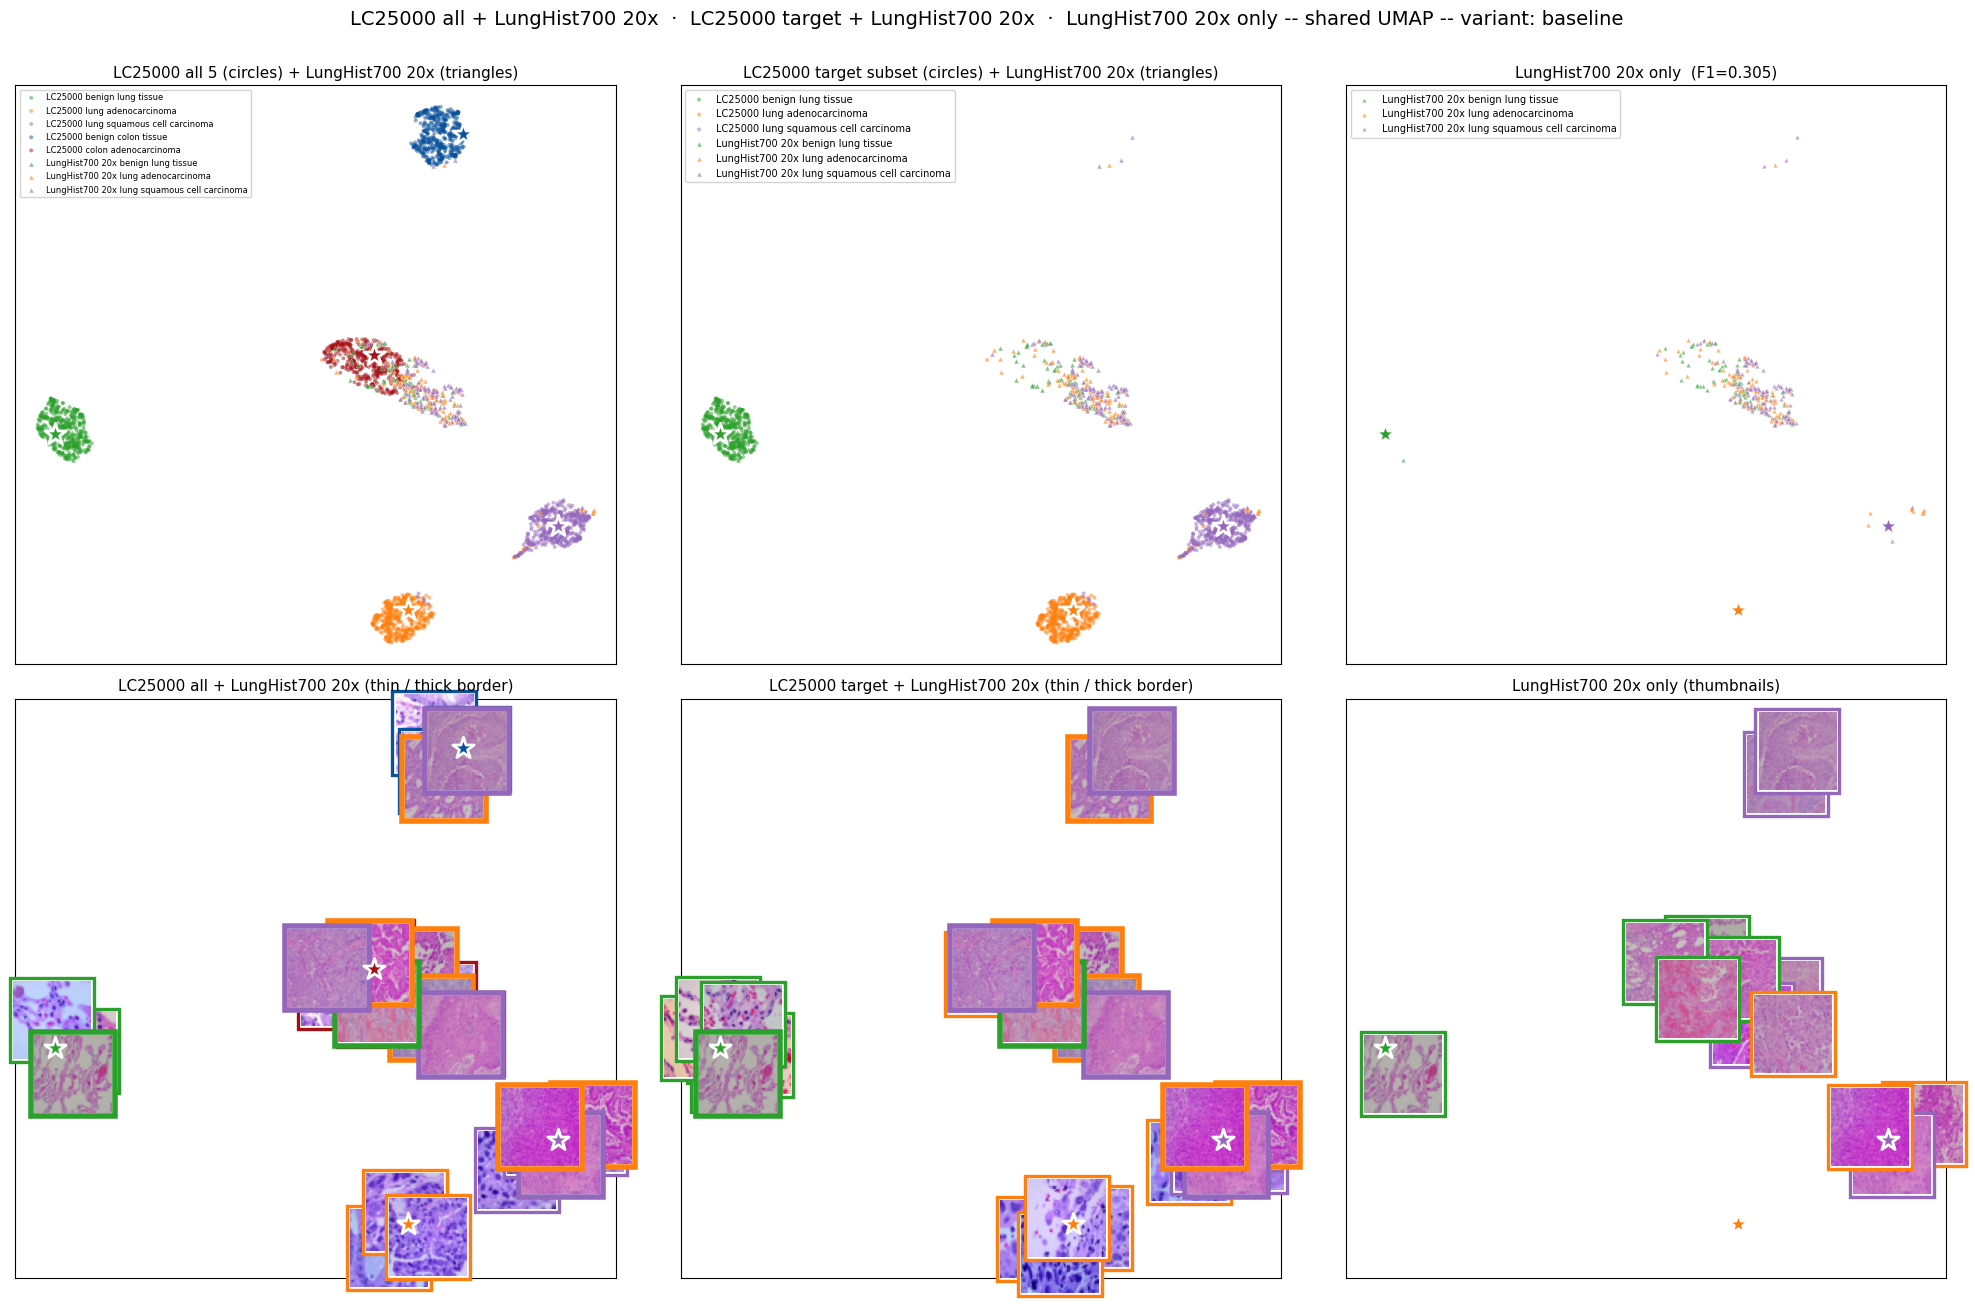
\includegraphics[width=0.95\textwidth]{../results/plots/exp_07_ood_eval/baseline_lunghist700_20x_ood_umap_grid.png}
    \caption{Baseline cross-distribution UMAP on LungHist700. LC25000 image embeddings (dots) and LungHist700 image embeddings (triangles) projected into the same 2-D fit.}
    \label{fig:baseline-lung-umap}
\end{figure}

The Chaoyang dataset sits between these two regimes (Figure~\ref{fig:baseline-chaoyang-umap}). The two colon classes are partially separated in the projected space, and the Chaoyang triangles cluster in a region adjacent to --- but not co-located with --- the matching LC25000 colon clusters: enough signal for partial transfer, with a measurable cost from the cross-hospital distribution gap. Together with NCT and LungHist700, this exposes two distinct generalisation regimes for the experiments that follow. There is a colon regime, where frozen ImageNet features carry good-enough structure for partial transfer, and a lung regime, where they carry no usable structure at all. The central question the rest of this chapter is built around: is the lung-side failure about the encoder's architecture, about its supervised pretraining on natural images, or about the absence of histopathology data in pretraining? The DINOv2 control (general-domain self-supervised pretraining, no histology) and the PLIP backbone (ViT pretrained on histopathology image--text pairs) jointly decompose that question, and the headline answer arrives in §\ref{sec:results-image-encoder}.

\begin{figure}[H]
    \centering
    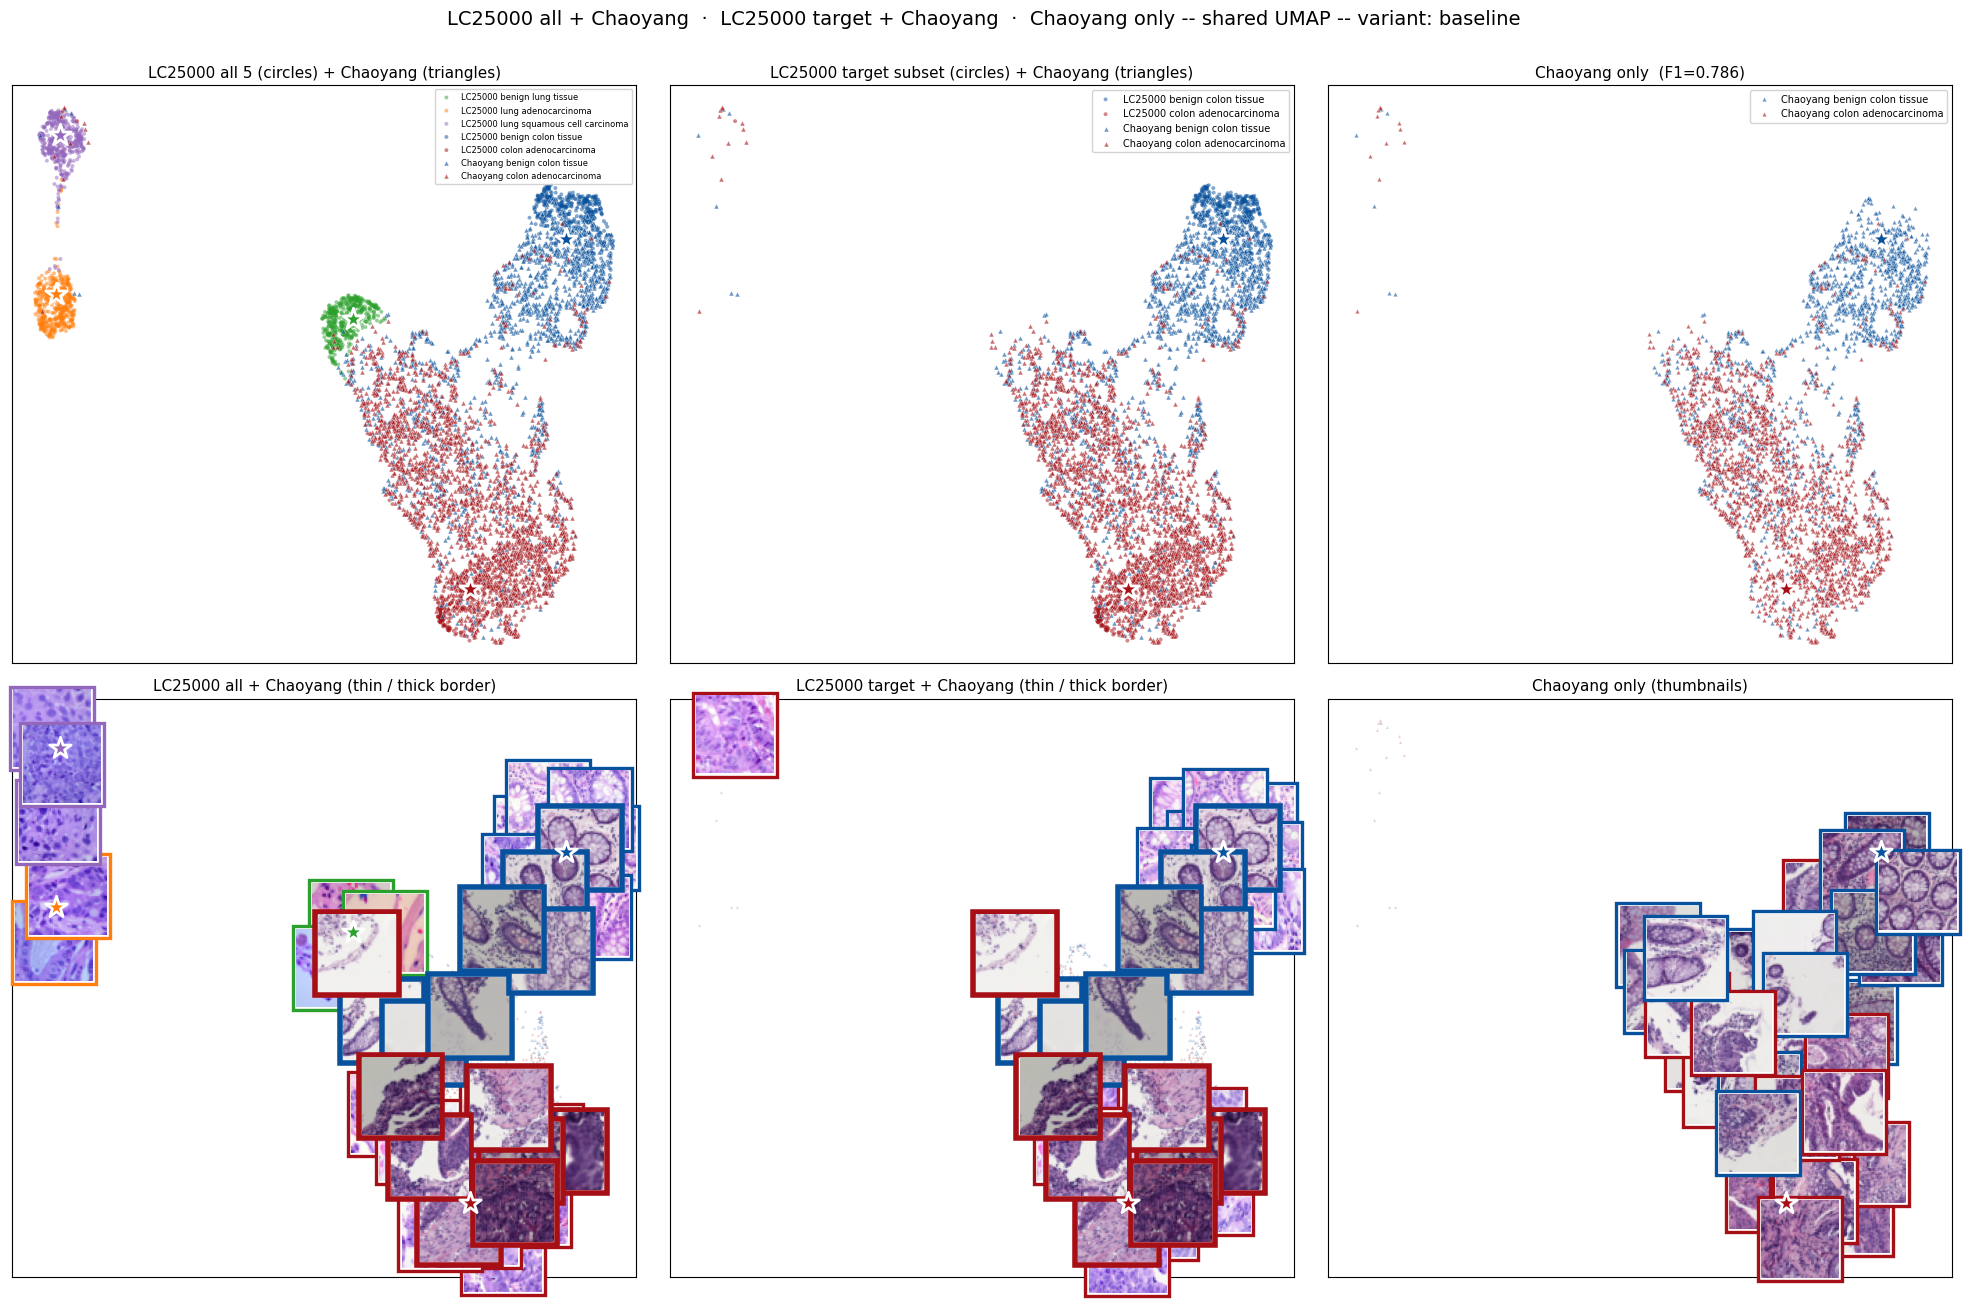
\includegraphics[width=0.95\textwidth]{../results/plots/exp_07_ood_eval/baseline_chaoyang_ood_umap_grid.png}
    \caption{Baseline cross-distribution UMAP on Chaoyang. LC25000 image embeddings (dots) and Chaoyang image embeddings (triangles) projected into the same 2-D fit.}
    \label{fig:baseline-chaoyang-umap}
\end{figure}


% ============================================================
\FloatBarrier
\section{Stain normalization}
\label{sec:results-stain}

\subsection{Configuration}

The stain-normalisation experiment keeps the baseline pipeline architecture identical to §\ref{sec:results-baseline-config} and changes only the image-input distribution. Every LC25000 training image is Macenko-normalised~\cite{macenko2009stain} against a single fixed reference patch: the first \texttt{NORM} tile from NCT-CRC-HE-7K, abbreviated ``NCT-NORM'' below.

The choice of reference matters operationally. NCT-CRC is distributed already Macenko-normalised against an unpublished Kather-team reference~\cite{kather2019nct}; by Macenko-normalising LC25000 onto an NCT-CRC tile, we land the training distribution in approximately the colour space NCT-CRC arrives in at release, which lets NCT-CRC be fed raw at evaluation and avoids the double-Macenko regime that historically zeroed out the OOD F1 in an earlier version of this experiment. Chaoyang and LungHist700, by contrast, arrive in their native un-normalised palettes, so for those two datasets the same Macenko(NCT-NORM) transform is applied at inference to bring them into the model's training-stain space. An alternative reference drawn from Chaoyang or LungHist700 --- the latter being the most stain-distinct of the three external datasets --- would have re-introduced the double-Macenko problem on NCT-CRC and required a separate retraining run for each reference tested; the NCT-NORM reference is therefore picked for methodological consistency rather than per-dataset optimisation, and reference rotation as an ablation axis is documented as a limitation in Chapter~\ref{chp:conclusion}.

Reinhard and Vahadane were also explored as alternative normalisations in an exploratory pass but did not advance to the full external-evaluation ablation. Vahadane's NMF solver fails to converge on a fraction of LC25000 patches --- visible in Figure~\ref{fig:stain-before-after}(d), where the bottom-row \texttt{colon\_aca} cell re-renders near-blank. Reinhard is a Lab-space colour-statistics transfer rather than a stain-decomposition method, included in the figure for visual comparison only.

\begin{figure}[ht]
    \centering
    \begin{minipage}[t]{0.23\textwidth}
        \centering
        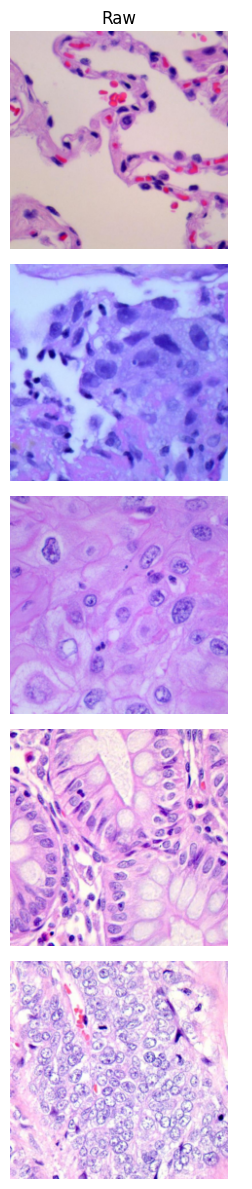
\includegraphics[width=\textwidth]{../results/plots/stain_raw_examples.png}
        \par\vspace{2pt}\footnotesize (a) Raw.
    \end{minipage}\hfill
    \begin{minipage}[t]{0.23\textwidth}
        \centering
        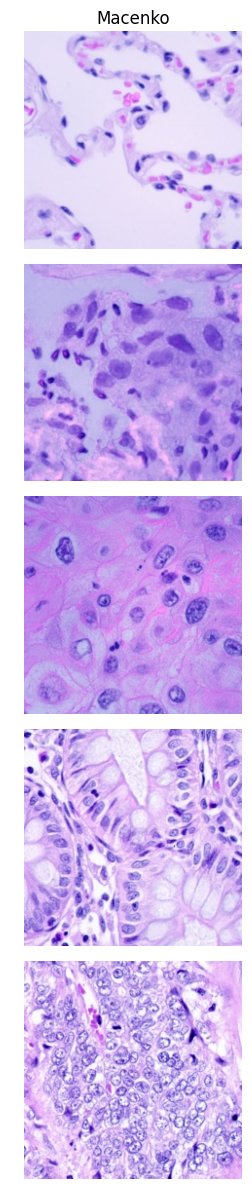
\includegraphics[width=\textwidth]{../results/plots/stain_macenko_normalized_only.png}
        \par\vspace{2pt}\footnotesize (b) Macenko.
    \end{minipage}\hfill
    \begin{minipage}[t]{0.23\textwidth}
        \centering
        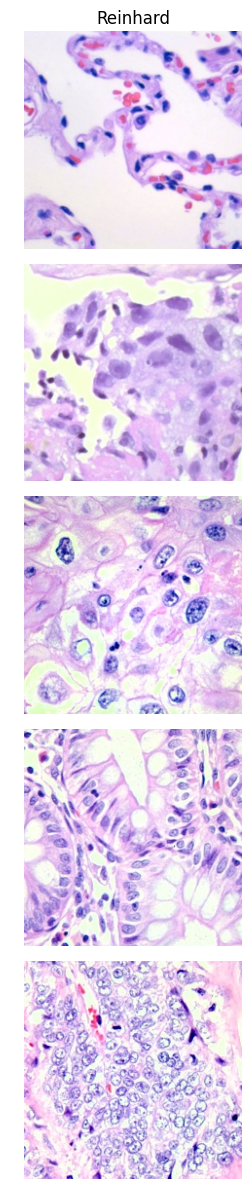
\includegraphics[width=\textwidth]{../results/plots/stain_reinhard_normalized_only.png}
        \par\vspace{2pt}\footnotesize (c) Reinhard.
    \end{minipage}\hfill
    \begin{minipage}[t]{0.23\textwidth}
        \centering
        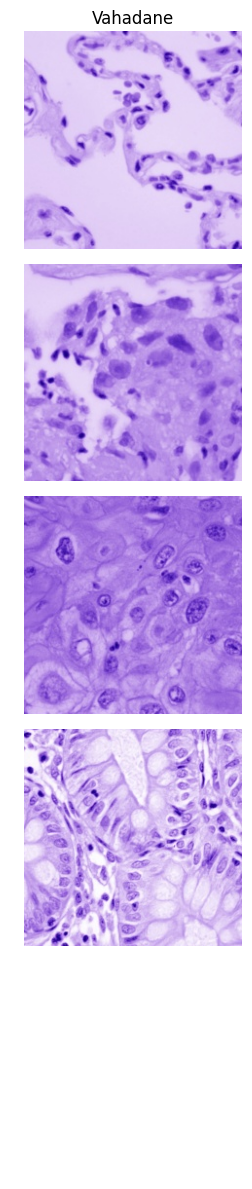
\includegraphics[width=\textwidth]{../results/plots/stain_vahadane_normalized_only.png}
        \par\vspace{2pt}\footnotesize (d) Vahadane.
    \end{minipage}
    \caption{Stain normalization, one example per class. Column (a) shows the raw inputs (identical across methods, shown once for compactness); columns (b)--(d) show the same inputs after Macenko, Reinhard, and Vahadane normalization respectively. The bottom-row colon\_aca cell in column (d) shows the Vahadane NMF solver failing to converge and re-rendering near-blank, an instability discussed in the interpretation.}
    \label{fig:stain-before-after}
\end{figure}

\subsection{Generalization to external datasets}

On LC25000 the Macenko-trained checkpoint saturates at $0.986$ macro-F1, alongside the baseline and every other trained variant in this study --- in-distribution does not discriminate this lever, so the substantive comparison is the external evaluation reported in Table~\ref{tab:stain-3way}.

\begin{table}[H]
    \centering
    \small
    \begin{tabular}{|l|c|c|c|}
    \hline
    \textbf{External dataset} & \textbf{Baseline F1} & \textbf{Macenko F1} & \textbf{Delta} \\ \hline
    NCT-CRC-HE-7K (close-shift colon)         & $0.866$ & $0.844$ & $-0.022$ \\ \hline
    Chaoyang (different-hospital colon)       & $0.786$ & $0.816$ & $+0.030$ \\ \hline
    LungHist700 (different-source lung, 20$\times$)  & $0.305$ & $0.325$ & $+0.020$ \\ \hline
    \end{tabular}
    \caption{Macenko(NCT-NORM) vs baseline on the three external evaluation datasets.}
    \label{tab:stain-3way}
\end{table}

\textbf{The lever's direction is data-dependent.} On the two datasets that arrive in their native stain palette --- Chaoyang ($+0.030$ F1) and LungHist700 ($+0.020$ F1), both receiving Macenko at inference --- normalisation moves the input closer to the model's training distribution and the frozen ImageNet ResNet50 produces better features. On NCT-CRC the picture inverts: NCT was already in approximately the target stain space at release, so training-time Macenko introduced a non-linear shift the frozen backbone could not absorb, and the eval-time pass-through cannot recover the small cost paid ($-0.022$ F1).

The magnitude is modest, even where the lever helps. The $+0.020$--$+0.030$ F1 gains on Chaoyang and LungHist700 are real but small; by comparison, swapping the image encoder to PLIP (§\ref{sec:results-image-encoder}) gains $+0.027$ on Chaoyang and \textbf{$\mathbf{+0.335}$ on LungHist700 --- an order of magnitude larger}. At the frozen-backbone scale evaluated here, stain normalisation is a useful but not dominant lever, and the protocol lesson worth carrying forward is the asymmetric application: Macenko is applied at inference only on inputs that arrive in their native stain palette, since doubling on a pre-normalised target is what historically broke the OOD F1 in this experiment.


% ============================================================
\section{PLIP zero-shot reference}
\label{sec:results-plip-zeroshot}

\subsection{Configuration}
\begin{itemize}
    \item Visual Transformer (ViT-B/32) with PLIP's OpenPath pretraining, paired with PLIP's matching text encoder. Both frozen.
    \item Evaluated zero-shot --- no LC25000 supervision, no projection head trained on our data. Uses PLIP's own image and text encoders straight from the model release.
    \item Class prediction = cosine similarity to the five LC25000 class-prompt embeddings produced by PLIP's text encoder, argmax.
    \item Evaluated on the same training-source test split and the same external datasets as every other variant in this chapter.
    \item \textbf{Role in the chapter}: a reference point. PLIP zero-shot isolates the value of pathology pretraining alone --- without any of our LC25000 fine-tuning --- and shows what an off-the-shelf domain-pretrained model gives you on these tasks.
\end{itemize}

\subsection{Training source results}
\begin{itemize}
    \item Macro-F1 on LC25000: \textbf{0.700}.
    \item Pathology pretraining alone (without any LC25000 supervision) clears the saturation null that every \emph{trained} variant reaches at $\sim 0.99$ by $\sim 0.30$ F1 in the other direction --- but it is the only variant in the chapter where in-distribution numbers are informative, because PLIP zero-shot has no LC25000 supervision to drive the saturation.
    \item Per-class gains concentrate on benign tissues; cancer subtypes are essentially tied with baseline. The improvement is image-side: PLIP produces visibly better class clusters (Figure~\ref{fig:plip-umap}) but the class-prompt embeddings still collapse, same short-prompt degeneracy as the baseline.
\end{itemize}

\begin{figure}[ht]
    \centering
    \begin{minipage}[t]{0.48\textwidth}
        \centering
        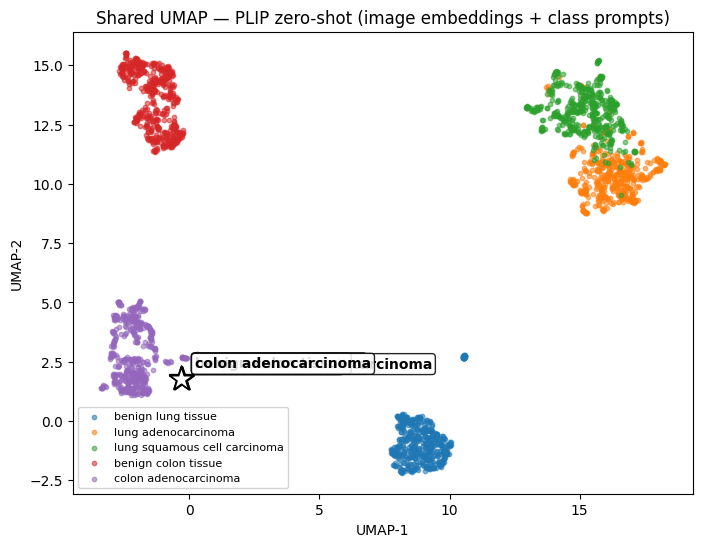
\includegraphics[width=\textwidth]{../results/plots/plip_zeroshot_umap.png}
        \par\vspace{2pt}\footnotesize (a) PLIP zero-shot.
    \end{minipage}\hfill
    \begin{minipage}[t]{0.48\textwidth}
        \centering
        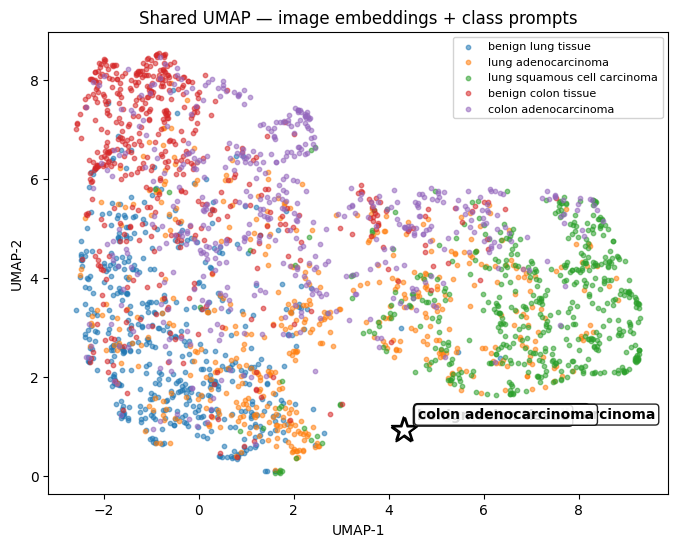
\includegraphics[width=\textwidth]{../results/plots/baseline_umap.png}
        \par\vspace{2pt}\footnotesize (b) Baseline (for comparison).
    \end{minipage}
    \caption{Training-source UMAP comparison. PLIP zero-shot (a) shows visibly tighter, more separated class clusters than the baseline (b) without any LC25000 supervision --- the gain is image-side.}
    \label{fig:plip-umap}
\end{figure}

\subsection{Generalization to external datasets}

\begin{table}[ht]
    \centering
    \small
    \begin{tabular}{|l|c|c|c|c|}
    \hline
    \textbf{Dataset (organ)} & \textbf{Macro-F1} & \textbf{Accuracy} & \textbf{Bal.\ acc.} & \textbf{Weighted F1} \\ \hline
    NCT-CRC-HE-7K (colon)            & 0.661 & 0.557 & 0.610 & 0.679 \\ \hline
    Chaoyang (colon)                 & \textbf{0.731} & 0.737 & 0.761 & 0.727 \\ \hline
    LungHist700 (lung, 20$\times$)   & 0.544 & 0.621 & 0.567 & 0.583 \\ \hline
    \end{tabular}
    \caption{PLIP zero-shot generalization across the three external datasets. No LC25000 supervision; class prediction by cosine similarity to PLIP-encoded prompts.}
    \label{tab:plip-zeroshot-ood}
\end{table}

\begin{itemize}
    \item \textbf{Chaoyang $>$ NCT.} PLIP zero-shot scores higher on Chaoyang ($0.731$) than on NCT-CRC ($0.661$), opposite of the pattern for every LC25000-trained variant (where NCT is the easier external dataset). Plausible reason: NCT-CRC is Macenko-normalised at release, pushing it away from the natural-staining distribution PLIP saw in OpenPath; Chaoyang's natural-stain images are stylistically closer to PLIP's pretraining corpus.
    \item \textbf{LungHist700 $= 0.544$.} The interesting cell. PLIP zero-shot has no LC25000 lung supervision yet outperforms the LC25000-trained ResNet50 variants ($0.305$) by $+0.239$ F1 on lung. Per-class recall: benign $0.16$ / AdC $0.69$ / SqC $0.84$ --- biased toward squamous like the ResNet50 variants, but not nearly as collapsed.
    \item Smallest training-source $\to$ external drop overall ($-0.04$ on NCT) --- the ``pretrained generalist'' pattern: never the best, never the worst, but consistent across distributions.
\end{itemize}

\subsection{What we learned}
\begin{itemize}
    \item Pathology pretraining produces a \emph{meaningfully better image representation} (visible directly in the UMAP) even without LC25000 supervision.
    \item PLIP's off-the-shelf prompt geometry is weak for our specific 5-class LC25000 vocabulary --- this decouples ``the image representation is useful'' from ``the off-the-shelf classifier works''.
    \item Section~\ref{sec:results-image-encoder} returns to this distinction by keeping PLIP's image representation but replacing its prompt geometry with a projection head trained on LC25000.
\end{itemize}


% ============================================================
\section{Foundational model vs plain classifier}
\label{sec:results-foundational-vs-plain}

\subsection{Configuration}
\begin{itemize}
    \item Same frozen ResNet50 image encoder as the baseline.
    \item Drops the CLIP paradigm entirely: no text encoder, no projection heads, no learnable temperature, no contrastive loss.
    \item Replaces it with a non-CLIP closed-set classifier: ResNet50 $\to$ global average pooling $\to$ BatchNorm $\to$ Dense(5) trained with sparse cross-entropy.
    \item Isolates what the CLIP paradigm itself contributes once the image encoder, data, and adaptation budget are held constant. Tests RQ2 (the foundational-model premise).
\end{itemize}

\subsection{Training source results}
\begin{itemize}
    \item Macro-F1 on LC25000: \textbf{0.6369} (vs baseline $0.6273$) \textit{(both numbers pre-bug-fix; post-fix both saturate at $\sim 0.99$, indistinguishable in-distribution)}.
    \item In-distribution the two architectures tie within noise. The choice between contrastive (CLIP) and direct supervised (plain classifier) is invisible when the image features are fixed and the training distribution is the evaluation distribution.
\end{itemize}

\subsection{Generalization to external datasets}
\begin{table}[ht]
    \centering
    \small
    \begin{tabular}{|l|c|c|c|c|}
    \hline
    \textbf{Variant} & \textbf{LC25000} & \textbf{NCT} & \textbf{Chaoyang} & \textbf{LungHist700} \\ \hline
    Baseline (CLIP InfoNCE)   & 0.996 & 0.866          & \textbf{0.786} & \textbf{0.305} \\ \hline
    Plain classifier (CE)     & 0.995 & \textbf{0.880} & 0.722          & 0.281 \\ \hline
    $\Delta$ (CLIP $-$ plain) & $-0.001$ & $-0.014$ & $+0.064$ & $+0.024$ \\ \hline
    \end{tabular}
    \caption{CLIP (baseline) vs plain classifier on the same frozen ResNet50 image encoder, macro-F1 across the training-source test split and three external datasets.}
    \label{tab:clip-vs-plain}
\end{table}

\begin{itemize}
    \item \textbf{Training source}: tied at $\sim 0.99$ (saturation null).
    \item \textbf{NCT-CRC (closest external dataset)}: plain CE marginally ahead by $+0.014$ F1.
    \item \textbf{Chaoyang (harder external)}: CLIP ahead by $+0.064$ F1 --- plain CE drops to last.
    \item \textbf{LungHist700 (hardest external)}: both variants collapse near 3-class chance; CLIP retains a marginal edge.
\end{itemize}

\noindent\textbf{Per-class signature on Chaoyang.} Plain CE shows benign precision $0.96$, benign recall $0.47$ (high precision, low recall --- the classifier is rarely predicting benign but is right when it does); adenocarcinoma precision $0.70$, recall $0.98$. The plain classifier is almost-degenerate ``predict adenocarcinoma'' under shift. The baseline CLIP variant is imperfect but balanced (benign $0.86$/$0.65$, adeno $0.76$/$0.92$), avoiding the collapse.

\subsection{What we learned}
\begin{itemize}
    \item CLIP and plain CE are \emph{interchangeable on easy distributions}; the choice of architecture is invisible when the model is evaluated on its training distribution.
    \item CLIP's edge appears \emph{under shift severity and grows with it}: $-0.014$ F1 on close-shift NCT (plain ahead), $+0.064$ on different-hospital Chaoyang (CLIP ahead), $+0.024$ on different-source LungHist700.
    \item \textbf{Mechanism}: same image encoder, same image features. The difference is the classifier geometry. The plain CE softmax learns class \emph{direction vectors} in feature space and is trained to maximise the logit margin; on shifted data those vectors don't move but the inputs sit in different regions, and the high-confidence softmax collapses into a single-class predictor. CLIP uses cosine similarity to class-prompt embeddings in an L2-normalized 256-d projection space, scaled by a learned temperature. Three effects make this geometry more robust:
    \begin{itemize}
        \item Cosine similarity is bounded in $[-1, 1]$ --- no unbounded margin for the model to over-extrapolate.
        \item The L2-normalized space concentrates features near the unit sphere; samples that drift in absolute feature space remain closer in \emph{angular} terms to the prompt anchors.
        \item The learned temperature $\tau$ acts as a soft regularizer on the cosine distribution: it tempers extreme confidence without removing the ranking signal.
    \end{itemize}
    \item This is a property of the CLIP \emph{paradigm}, not of any specific encoder. The same geometry was designed for the open-vocabulary regime (new class prompts at inference time) and incidentally protects against distribution shift on closed-set tasks. \textbf{This validates RQ2's foundational-model framing}: CLIP earns its complexity not at peak in-distribution accuracy, but in the open-vocabulary capabilities (retrieval, prompt-tuning at inference) and the robustness-under-shift behaviour shown here.
\end{itemize}


% ============================================================
\section{Text encoder pretraining}
\label{sec:results-text-encoder}

\subsection{Configuration}
\begin{itemize}
    \item Same arch / loss / prompts / split as the baseline; only the frozen text encoder changes.
    \item Three encoders: \texttt{bert-base-uncased} (the baseline's text encoder), BioBERT, PubMedBERT.
    \item Two prompt strategies: \textbf{name\_only} (just the class name, e.g.\ \texttt{``benign lung tissue''}) and \textbf{composed} (\texttt{``A histopathology image of \{class\}.''}, the baseline format).
    \item $3 \times 2 = 6$ cells. All three encoders are BERT-family, all produce 768-d hidden state, all tokenize through BERT-family WordPiece tokenizers.
    \item Tests RQ4 (does biomedical text pretraining help under short class-name prompts?).
\end{itemize}

\subsection{NCT-CRC grid (6 cells)}
\begin{table}[ht]
    \centering
    \small
    \begin{tabular}{|l|c|c|c|}
    \hline
    \textbf{Cell} & \textbf{LC25000} & \textbf{NCT-CRC} & \textbf{$\Delta$ vs baseline NCT} \\ \hline
    BERT + name\_only       & 0.999 & 0.821 & $-0.045$ \\ \hline
    BERT + composed         & 0.999 & 0.863 & $-0.003$ \\ \hline
    BioBERT + name\_only    & 0.998 & 0.840 & $-0.026$ \\ \hline
    BioBERT + composed      & 0.998 & 0.818 & $-0.048$ \\ \hline
    PubMedBERT + name\_only & 0.995 & 0.855 & $-0.011$ \\ \hline
    PubMedBERT + composed   & 0.996 & 0.808 & $-0.058$ \\ \hline
    \end{tabular}
    \caption{6-cell biomedical text encoder ablation, macro-F1 on NCT-CRC. \textbf{None of the 6 cells beats the baseline ($0.866$ on NCT).} LC25000 in-distribution saturates uniformly; all generalization numbers land in the $0.81$--$0.86$ band. The BERT + composed cell is essentially baseline (same architecture, same prompt template); the best \emph{biomedical} cell --- PubMedBERT + name\_only at $0.855$ --- still trails baseline by $-0.011$ F1.}
    \label{tab:text-encoder}
\end{table}

\begin{figure}[ht]
    \centering
    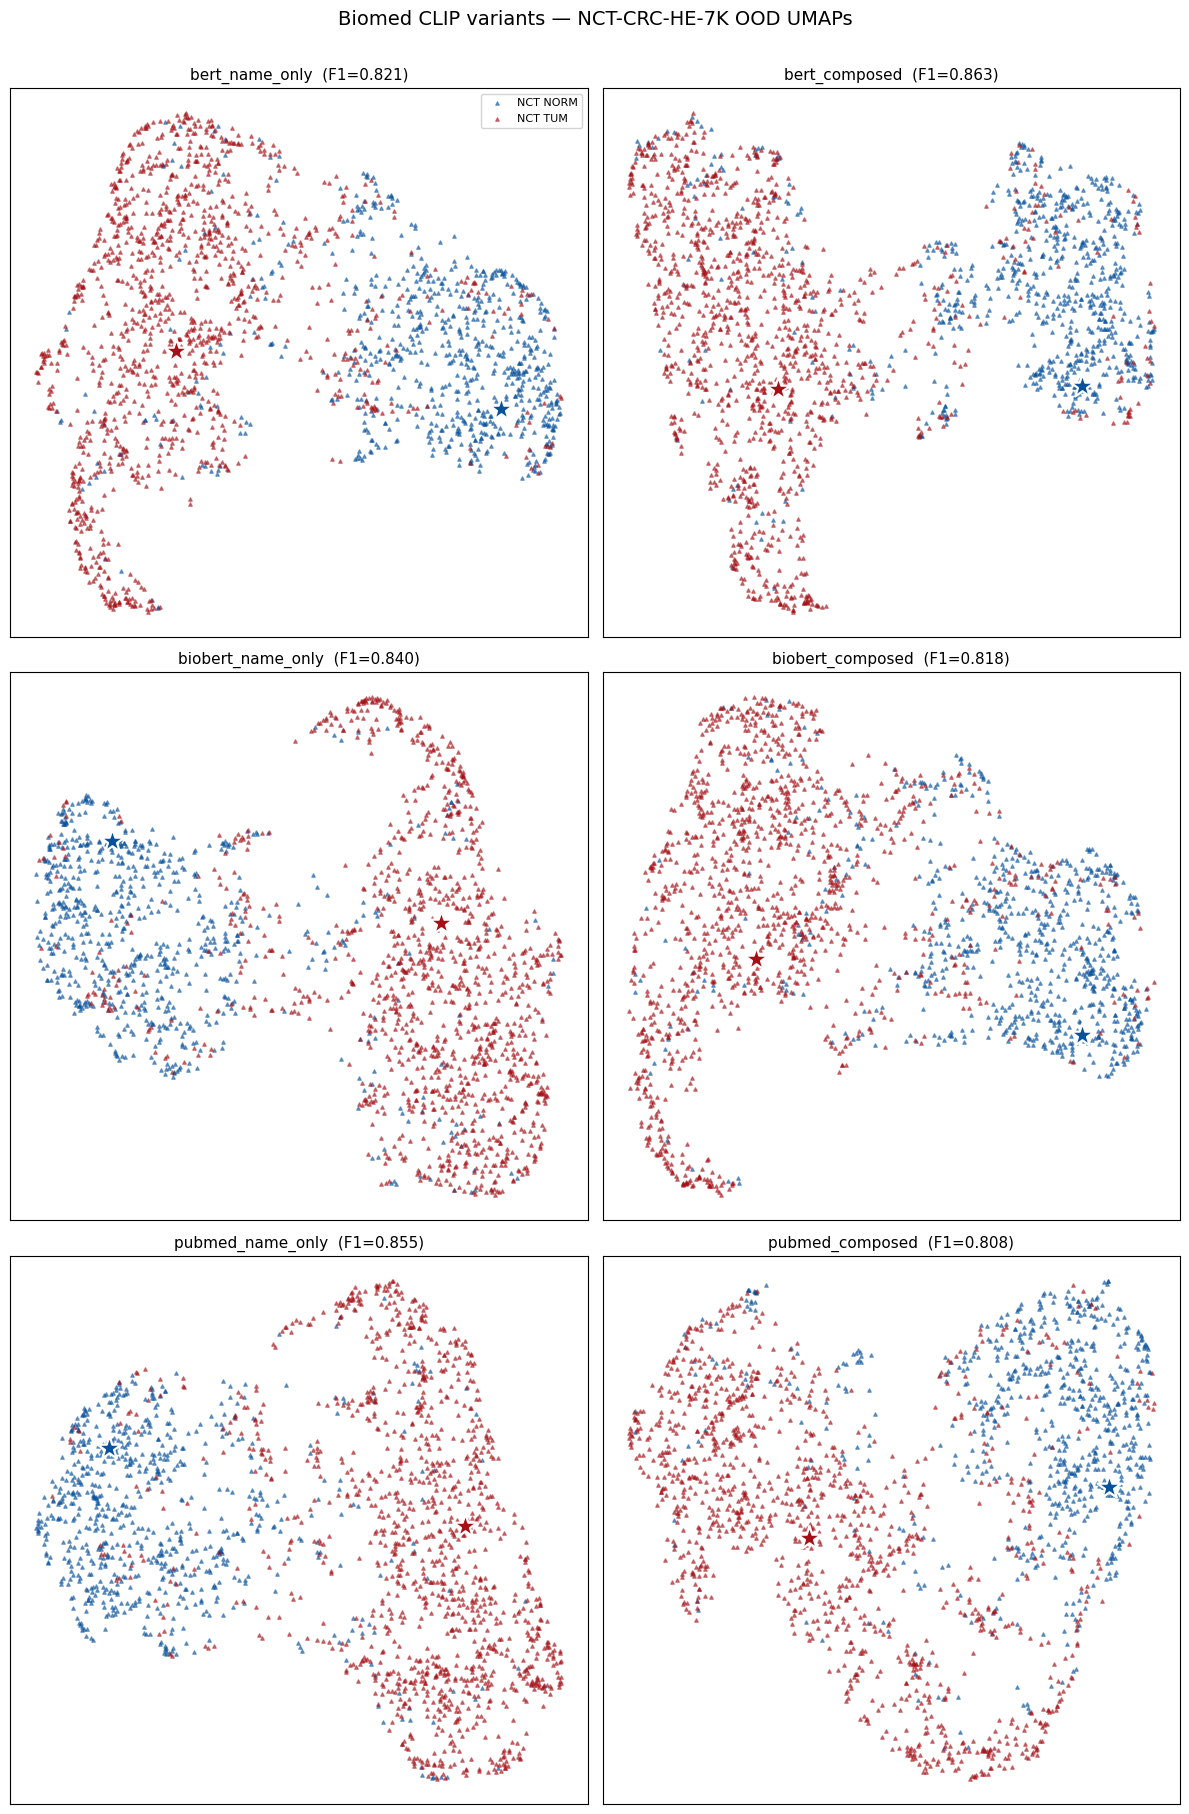
\includegraphics[width=0.95\textwidth]{../results/plots/exp_07_ood_eval/biomed_ood_umap_grid.png}
    \caption{6-cell UMAP grid (one panel per BERT/BioBERT/PubMedBERT $\times$ name\_only/composed cell), cross-distribution view on NCT-CRC. The clusters are qualitatively similar across cells, consistent with the lack of meaningful F1 separation in Table~\ref{tab:text-encoder}.}
    \label{fig:biomed-umap}
\end{figure}

\begin{itemize}
    \item LC25000 in-distribution: all cells saturate uniformly. The training-source axis does not discriminate these encoders.
    \item NCT generalization: all 6 cells land in the $0.81$--$0.86$ band. None beats the baseline.
\end{itemize}

\subsection{Generalization to Chaoyang and LungHist700}
\begin{itemize}
    \item The best biomedical cell on NCT --- PubMedBERT + name\_only --- was extended to Chaoyang and LungHist700 to test whether biomedical text encoders carry any advantage under heavier shift:
\end{itemize}

\begin{table}[ht]
    \centering
    \small
    \begin{tabular}{|l|c|c|c|}
    \hline
    \textbf{External dataset} & \textbf{Baseline F1} & \textbf{PubMedBERT+name\_only F1} & \textbf{Delta} \\ \hline
    NCT-CRC-HE-7K (close-shift colon)               & $0.866$ & $0.855$ & $-0.011$ \\ \hline
    Chaoyang (different-hospital colon)             & $0.786$ & $0.795$ & $+0.009$ \\ \hline
    LungHist700 (different-source lung, 20$\times$)  & $0.305$ & $0.279$ & $-0.026$ \\ \hline
    \end{tabular}
    \caption{Best biomedical text-encoder cell (PubMedBERT + name\_only) vs baseline on the three external evaluation datasets. The biomedical text encoder ties baseline on Chaoyang (within noise) and regresses on both NCT and LungHist700. No measurable transfer benefit on any of the three datasets.}
    \label{tab:text-encoder-3way}
\end{table}

\begin{itemize}
    \item \textbf{No transfer.} The best biomedical cell ties baseline on Chaoyang ($+0.009$, within noise) and \emph{regresses} on LungHist700 ($-0.026$). Combined with the NCT result ($-0.011$), no biomedical-text-encoder configuration tested produces a measurable gain on any external dataset.
    \item \textbf{LungHist700 collapse signature.} Both baseline and PubMedBERT+name\_only collapse on lung, just to different classes. Baseline predicts ``lung squamous cell carcinoma'' on most inputs in the degenerate regime; PubMedBERT+name\_only also collapses to lung\_scc but harder ($\sim 92$\% of predictions). In both cases the per-class recall on the other two lung classes is near-zero --- a single-class predictor regime where the text encoder choice only affects how \emph{sharply} the collapse manifests.
\end{itemize}

\subsection{What we learned}
\begin{itemize}
    \item Biomedical text pretraining does \emph{not} help on this task at frozen-backbone scale with short class-name prompts. Confirmed across three external datasets: PubMedBERT + name\_only (the best biomedical cell on NCT) ties baseline on Chaoyang and regresses on both NCT and LungHist700.
    \item \textbf{Mechanism --- why doesn't ``a more domain-aware text encoder'' improve results?} Three converging reasons:
    \begin{itemize}
        \item \emph{The projection head absorbs encoder-specific differences.} BERT, BioBERT, and PubMedBERT all start from different 768-d embedding spaces, but they all get pulled through the same projection head trained on LC25000. The head learns to map any reasonable starting embedding to useful class anchors. With only 5 LC25000 classes to separate, this is an easy adaptation regardless of where the starting embeddings sit.
        \item \emph{Short class-name prompts don't expose biomedical-vocabulary richness.} Biomedical pretraining adds value most when domain vocabulary actually appears --- clinical notes, paper abstracts, multi-sentence text. Strings like \texttt{``colon adenocarcinoma''} tokenize into 2--3 wordpieces that any BERT-family encoder handles competently. There is no rare-medical-term upside for biomedical pretraining to surface.
        \item \emph{CLIP's shift robustness is geometric, not domain-knowledge driven.} As argued in Section~\ref{sec:results-foundational-vs-plain}, CLIP's edge under shift comes from the cosine + L2-norm + temperature classifier geometry, which is independent of the text encoder. Swapping in a more medically-aware text encoder doesn't change the classifier geometry; it changes the starting position of the prompt anchors, which the projection head then re-maps anyway.
    \end{itemize}
    \item \textbf{Small but interesting secondary observation}: vanilla BERT prefers the longer \textbf{composed} prompt format; biomedical encoders prefer \textbf{bare class names}. Plausible mechanism: biomedical pretraining made strings like \texttt{``colon adenocarcinoma''} carry strong signal on their own, while adding generic boilerplate (\texttt{``A histopathology image of \ldots''}) dilutes the prompt embedding for biomedical encoders. Not enough to flip any cell to winning --- but a useful methodological note for short-prompt design.
\end{itemize}


% ============================================================
\section{Image encoder pretraining}
\label{sec:results-image-encoder}

\subsection{Configuration}
\begin{itemize}
    \item Same arch / loss / prompts / split / text encoder (frozen BERT base) as the baseline. The only axis that changes is the image encoder's pretraining.
    \item Three image encoders compared, all frozen, trainable parameters limited to the projection head + temperature:
    \begin{itemize}
        \item \textbf{ResNet50 (general-purpose, ImageNet pretraining)} --- the baseline.
        \item \textbf{Visual Transformer (ViT-B/32) with PLIP's OpenPath pretraining} --- a ViT pretrained on $\sim$208k histopathology image--text pairs scraped from Twitter.
        \item \textbf{Visual Transformer (ViT-B/14) with DINOv2 self-supervised pretraining} --- a ViT pretrained on $\sim$142M curated general natural images via self-distillation, no labels, no histopathology data.
    \end{itemize}
    \item \textbf{Role of DINOv2 in the comparison}: a control. PLIP differs from the baseline on multiple axes simultaneously (architecture: ViT vs CNN; objective: contrastive vs supervised; pretraining domain: histopathology vs natural images). DINOv2 isolates the ``ViT + self-supervised on general data'' axis from the ``histopathology pretraining specifically'' axis. If DINOv2 also breaks the baseline's lung collapse, the win is partly architectural; if it does not, the win is specifically about histopathology pretraining.
    \item \textbf{Caveat}: the two ViTs differ in patch size (PLIP B/32, DINOv2 B/14). At 224$\times$224 input this gives different feature granularity (49 vs 256 patch tokens). We discuss this as a confound in Methodology and address it as a limitation in Chapter~5.
\end{itemize}

\subsection{Training source results}
\begin{itemize}
    \item PLIP image encoder + LC25000 supervision: LC25000 macro-F1 $= 0.996$. Same saturation null as every other trained variant.
    \item DINOv2 image encoder + LC25000 supervision: LC25000 macro-F1 $= 0.989$. The saturation null holds even though DINOv2 has never seen labelled histology --- its pretraining is self-supervised on general natural images, with no class labels. Confirms that the in-distribution null is backbone-independent: the bottleneck on the meaningful axis is not what the image encoder ``knows about histology'' in the supervised sense; it is what kind of variation the encoder learned to be sensitive to.
\end{itemize}

\subsection{Generalization to external datasets}
\begin{table}[ht]
    \centering
    \small
    \begin{tabular}{|l|c|c|c|c|}
    \hline
    \textbf{Image encoder} & \textbf{LC25000} & \textbf{NCT} & \textbf{Chaoyang} & \textbf{LungHist700} \\ \hline
    ResNet50 (ImageNet)                              & 0.996 & 0.866 & 0.786 & 0.305 \\ \hline
    ViT-B/14 (DINOv2 / self-supervised)              & 0.989 & 0.855 & 0.776 & 0.457 \\ \hline
    \textbf{ViT-B/32 (PLIP / OpenPath)}              & \textbf{0.996} & \textbf{0.933} & \textbf{0.813} & \textbf{0.640} \\ \hline
    \end{tabular}
    \caption{Image encoder pretraining swap, macro-F1 across the training-source split and three external datasets. Everything except the image encoder is identical across rows.}
    \label{tab:image-encoder}
\end{table}

\begin{itemize}
    \item \textbf{NCT-CRC (close-shift colon)}: PLIP wins by $+0.067$ F1 over the ResNet50 baseline. DINOv2 lands at $-0.011$ vs baseline --- general-domain self-supervision does \emph{not} help on the easiest external dataset. The colon ceiling around $0.88$ that none of the other interventions could clear is broken specifically by changing the image encoder's pretraining \emph{domain}, not by architecture or self-supervision alone.
    \item \textbf{Chaoyang (different-hospital colon)}: PLIP wins by $+0.027$ F1; DINOv2 lands at $-0.010$ vs baseline. Same colon-side pattern as NCT: only histopathology pretraining helps; general SSL is interchangeable with ImageNet supervision.
    \item \textbf{LungHist700 (different-source lung)}: this is where the control pays off. PLIP wins by $+0.335$ F1 over baseline; DINOv2 wins by $+0.152$ F1. \emph{Roughly half of PLIP's lung advantage comes from architecture + self-supervised pretraining on general images; the other half comes from histopathology pretraining specifically.} DINOv2 partially rescues the lung collapse (per-class recall $0.46/0.52/0.40$, balanced) but does not match PLIP's full functional classifier ($0.51/0.49/0.91$).
\end{itemize}

\noindent\textbf{Per-class signature on LungHist700.} Both ResNet50 variants converge to the same degenerate predictor on lung tissue: baseline recall $0.19/0.07/0.89$ for normal/AdC/SqC, plain CE $0.15/0.05/0.91$ --- both predict ``squamous'' on $\sim 90$\% of inputs regardless of true class. \textbf{DINOv2-encoded variant: $0.46/0.52/0.40$} --- balanced across all 3 classes, no degenerate collapse, but lower peak per-class scores than PLIP. \textbf{PLIP-encoded variant: $0.51/0.49/0.91$} --- balanced \emph{and} retains the high squamous recall, the only variant that does both.

\begin{figure}[ht]
    \centering
    \begin{minipage}[t]{0.48\textwidth}
        \centering
        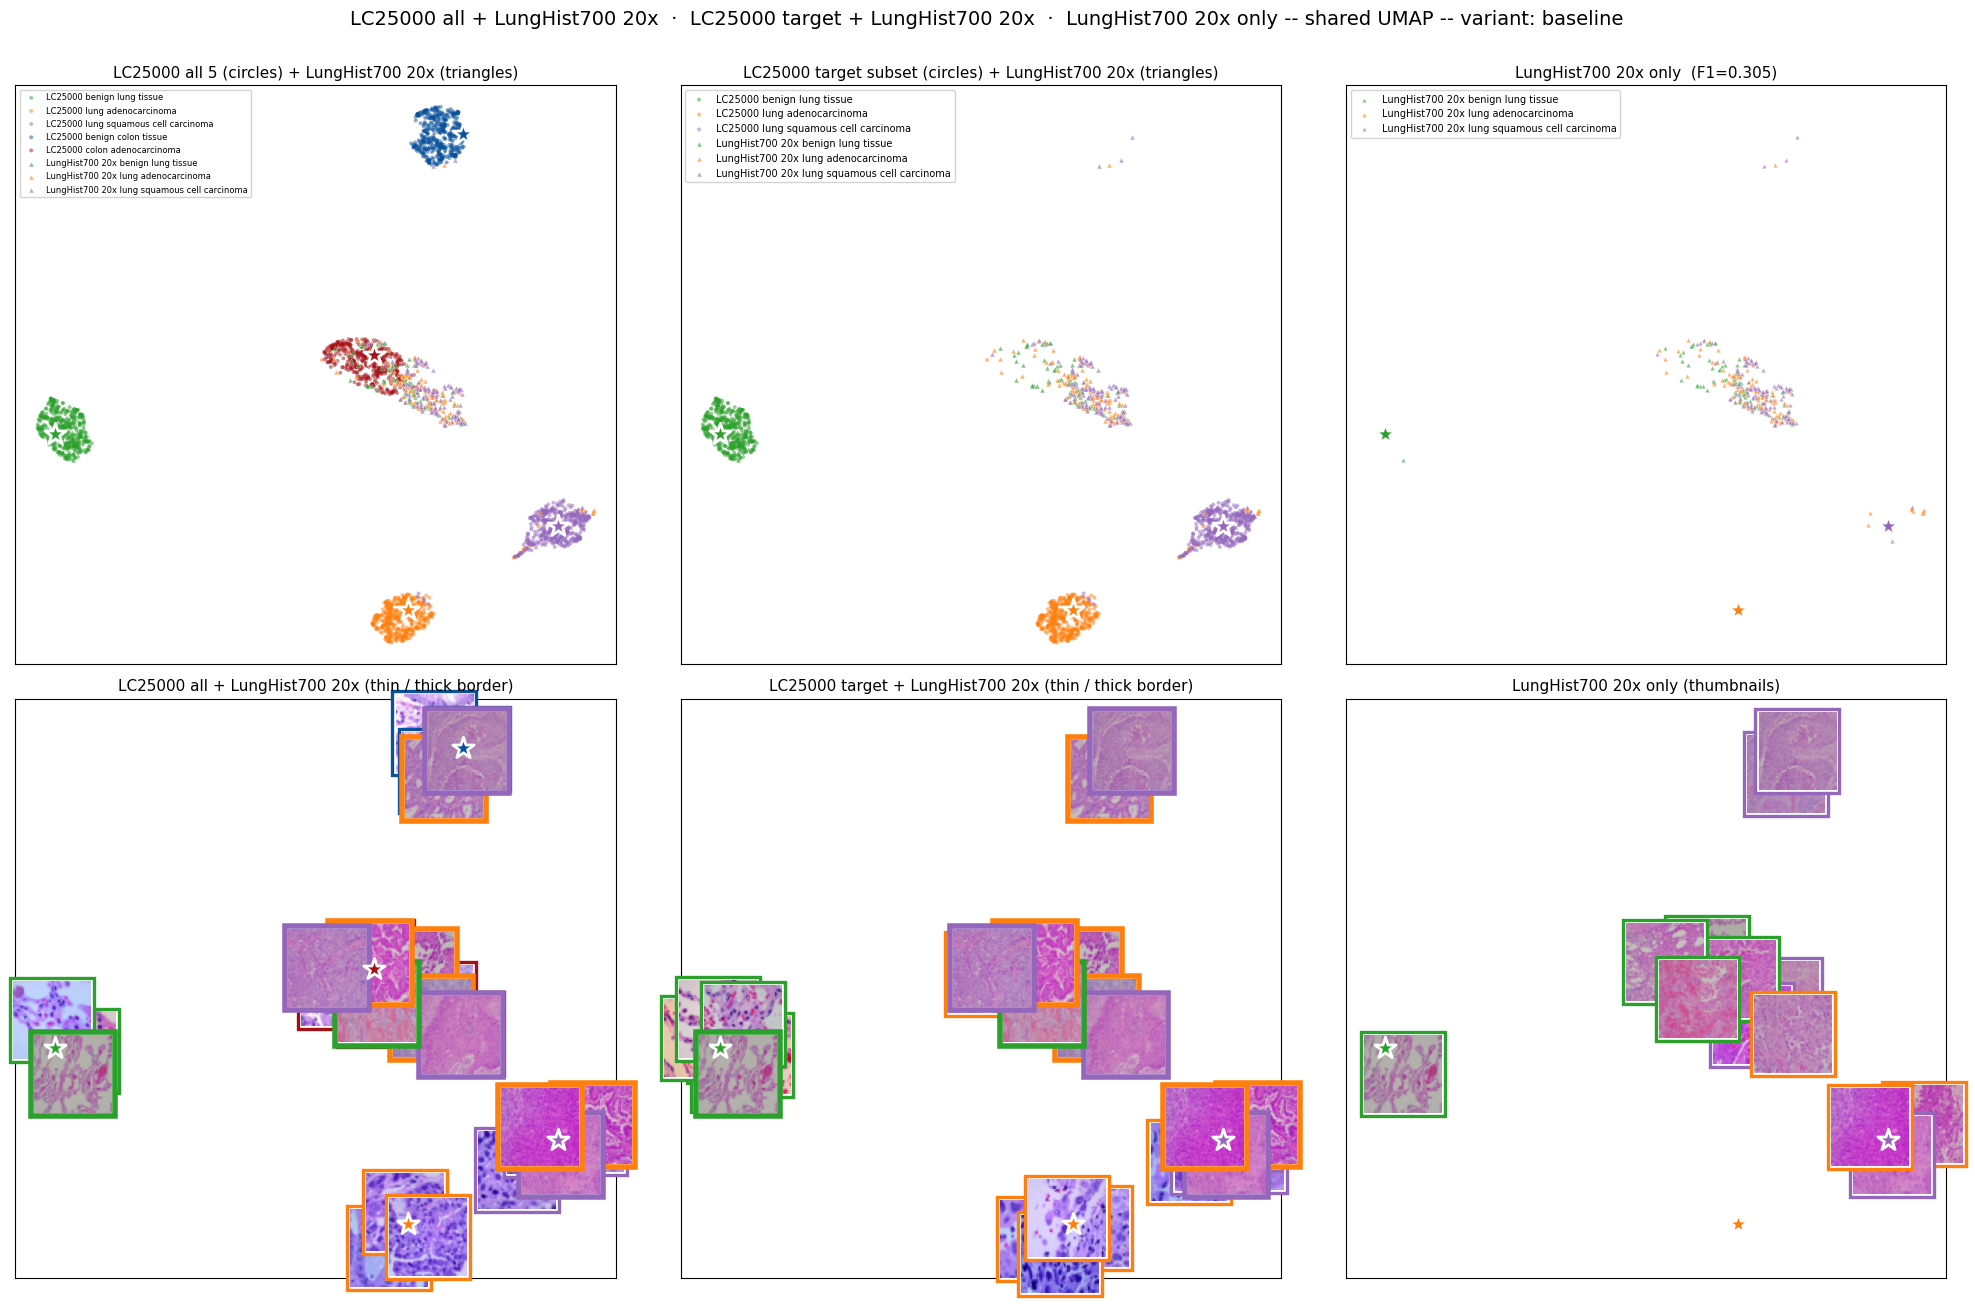
\includegraphics[width=\textwidth]{../results/plots/exp_07_ood_eval/baseline_lunghist700_20x_ood_umap_grid.png}
        \par\vspace{2pt}\footnotesize (a) ResNet50 baseline: a single tight blob, no internal class structure.
    \end{minipage}\hfill
    \begin{minipage}[t]{0.48\textwidth}
        \centering
        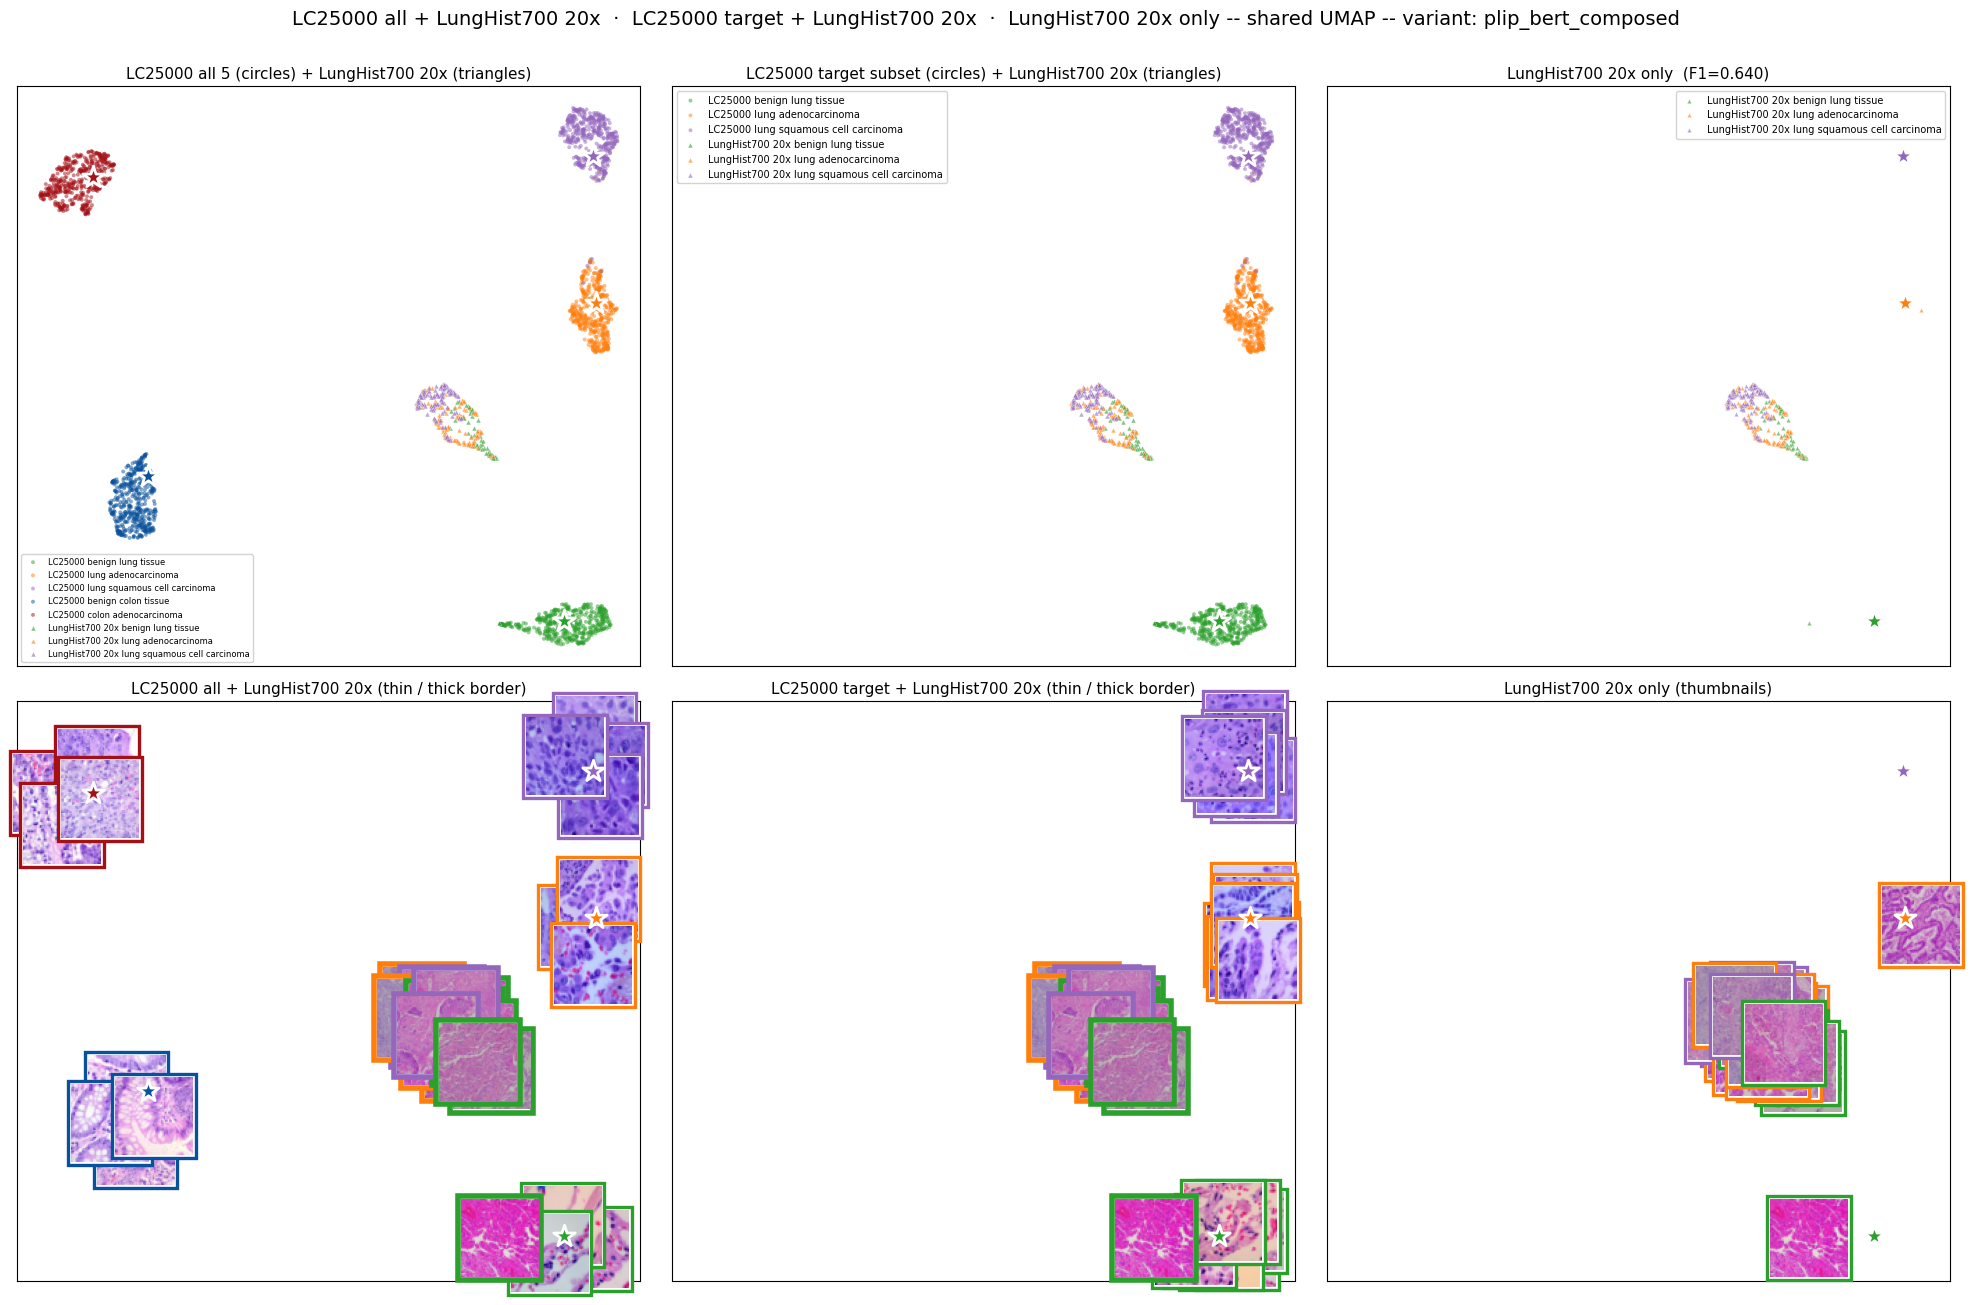
\includegraphics[width=\textwidth]{../results/plots/exp_07_ood_eval/plip_bert_composed_lunghist700_20x_ood_umap_grid.png}
        \par\vspace{2pt}\footnotesize (b) ViT-B/32 with PLIP pretraining: three visibly separated sub-clusters by class.
    \end{minipage}
    \caption{LungHist700 cross-distribution UMAP comparison --- the visual headline of this chapter. The ResNet50 baseline (a) places all 359 LungHist700 samples into a single tight cluster with no internal class structure; the PLIP-pretrained ViT (b) produces three visibly distinct sub-clusters by class, sitting adjacent to (but not co-located with) the matching LC25000 lung clusters.}
    \label{fig:image-encoder-umap-lung}
\end{figure}

\subsection{What we learned}
\begin{itemize}
    \item The \textbf{image encoder's pretraining is the dominant lever in this study}, but the DINOv2 control reveals that ``pretraining'' decomposes into two contributing components.
    \item Effect-size summary: PLIP gains over baseline by $+0.067$ F1 on close-shift colon, $+0.027$ on different-hospital colon, \textbf{$+0.335$ on different-source lung}. DINOv2 gains over baseline by $-0.011$ / $-0.010$ / $+0.152$ on the same three datasets.
    \item \textbf{On colon (NCT, Chaoyang)}: only histopathology pretraining moves the needle. General-domain self-supervised pretraining (DINOv2) lands within noise of ResNet50 supervised pretraining on natural images. The colon advantage is specifically about \emph{what} the encoder was pretrained on, not \emph{how}.
    \item \textbf{On lung (LungHist700)}: the DINOv2 and PLIP-zero-shot controls together yield a clean three-step decomposition of PLIP-backbone's $+0.335$ F1 gap. Baseline at $0.305$ $\to$ DINOv2 at $0.457$ ($+0.152$, ``ViT $+$ general-domain SSL'' contribution) $\to$ PLIP zero-shot at $0.544$ ($+0.087$, ``histopathology pretraining without LC25000 supervision'' contribution) $\to$ PLIP-backbone at $0.640$ ($+0.096$, ``LC25000 supervision on top of histopathology pretraining'' contribution). Three roughly comparable steps of $\sim 0.1$ F1 each, sequentially adding architecture/SSL, then domain, then task supervision.
    \item Why colon and lung behave differently, on the ResNet50 baseline: ImageNet supervision contains no histology. LC25000 supervision rescues ResNet50 features that happen to correlate with colon class labels in the LC25000 training distribution. That correlation transfers partially to NCT/Chaoyang (both colon, stylistically close). It does not transfer to lung tissue at all --- the lung-side ``success'' in-distribution is memorisation on the LC25000 lung subset, not learned lung tissue features.
    \item Why DINOv2 helps on lung but not colon: DINOv2's self-supervised pretraining on $\sim 142$M diverse natural images produces image features that are sensitive to a much broader range of local-texture variation than supervised ImageNet pretraining. That broader feature space provides \emph{enough} signal for LC25000 supervision + the projection head to construct a usable lung classifier, even though the encoder has never seen histology. On colon, where ResNet50 features were already enough for partial transfer, DINOv2's broader features do not help further --- the bottleneck on colon is the pretraining domain, not the architecture's feature breadth.
    \item Patch-size confound check: DINOv2 has more spatial detail than PLIP ($256$ vs $49$ patch tokens at the same 224$\times$224 input), but still loses on colon. The patch-size difference is therefore not the dominant factor here --- pretraining is.
\end{itemize}


% ============================================================
\section{Discussion}
\label{sec:results-discussion}

\subsection{Synthesis across experiments}
\begin{itemize}
    \item This chapter evaluated six interventions on a frozen general-purpose CLIP pipeline (ResNet50 + BERT). Five of the six (stain normalization, biomedical text encoders, plain-classifier substitution, the prompt-format variations within the text-encoder ablation) produce changes within $\sim 0.03$ F1 of the baseline on close-shift external evaluation (NCT) and at most $\sim 0.03$ F1 of improvement on the harder external datasets. Stain Macenko is the only input-side lever that moves the needle positively under shift ($+0.030$ on Chaoyang, $+0.020$ on LungHist700), but its magnitude is dominated by the image-encoder lever on the same datasets. The best biomedical text-encoder cell (PubMedBERT + name\_only) confirms the null result across all 3 external datasets --- ties baseline on Chaoyang, regresses on NCT and LungHist700.
    \item The sixth intervention --- replacing the image encoder's pretraining (Section~\ref{sec:results-image-encoder}) --- moves the headline metric by $+0.067$ on close-shift colon (NCT), $+0.027$ on different-hospital colon (Chaoyang), and \textbf{$+0.335$ on different-source lung (LungHist700)}, taking the lung result from a degenerate single-class predictor at $0.305$ to a functional 3-class classifier at $0.640$.
    \item The DINOv2 and PLIP-zero-shot controls together decompose that gain on lung into a clean ladder: $0.305$ (baseline) $\to$ $0.457$ (DINOv2: ViT $+$ SSL contribution, $+0.152$) $\to$ $0.544$ (PLIP zero-shot: histopath pretraining contribution, $+0.087$) $\to$ $0.640$ (PLIP-backbone: LC25000 supervision on top, $+0.096$). Three roughly equal steps of $\sim 0.1$ F1. On colon, the decomposition collapses --- DINOv2 ties baseline and PLIP zero-shot actually falls below baseline on Chaoyang ($0.731$ vs $0.786$) because LC25000 supervision was already enough.
    \item \textbf{The image encoder's pretraining is the dominant lever}, by roughly $5\times$ over the next-largest single lever on colon external evaluation. On lung, no head/loss/text-side intervention rescues a non-functional predictor at all; only changing the encoder does.
    \item The contemporary methods literature's emphasis on novel loss functions, text-side innovations, and stain harmonisation is not supported by this study at the frozen-backbone scale we evaluated.
\end{itemize}

\subsection{Secondary observations}
\begin{itemize}
    \item \textbf{Cross-organ regime change.} ResNet50 variants partially work on colon external data ($0.78$--$0.88$) but \emph{categorically fail} on lung ($\sim 0.30$, near 3-class chance). Mechanism: LC25000 supervision can rescue ResNet50 features that happen to correlate with colon class labels in LC25000, but cannot produce useful lung-tissue features within a frozen ImageNet ResNet50; the in-distribution lung ``success'' is memorisation. Per-organ external evaluation is therefore essential; aggregating across datasets hides the regime change.
    \item \textbf{Classification quality $\neq$ representation alignment.} Baseline CLIP achieves cross-dataset \emph{cluster alignment} but lower classification F1; PLIP achieves the highest F1 but leaves external samples in their own region of feature space. The contrastive objective optimises same-class-pair alignment; the cosine-classifier rule only needs alignment to the class-prompt direction. These are different geometric properties --- the right tradeoff depends on whether the downstream task is classification or representation-driven (retrieval, clustering, transfer).
    \item \textbf{Plain-classifier flip under shift.} Plain CE ties CLIP in-distribution and marginally wins NCT, but loses Chaoyang ($+0.064$ for CLIP) and LungHist700 ($+0.024$). High-confidence softmax classifiers degenerate into single-class predictors as shift severity grows (visible in the Chaoyang per-class signature); CLIP's cosine geometry doesn't. This supports the foundational-model framing of RQ2: CLIP earns its complexity in shift robustness, not in-distribution accuracy.
\end{itemize}

\subsection{Headline summary}
\begin{table}[ht]
    \centering
    \small
    \begin{tabular}{|l|c|c|c|c|}
    \hline
    \textbf{Variant} & \textbf{LC25000} & \textbf{NCT} & \textbf{Chaoyang} & \textbf{LungHist700} \\ \hline
    \textbf{ViT-B/32 (PLIP)}                  & \textbf{0.996} & \textbf{0.933} & \textbf{0.813} & \textbf{0.640} \\ \hline
    ViT-B/14 (DINOv2)                          & 0.989 & 0.855 & 0.776 & 0.457 \\ \hline
    Baseline (ResNet50 + BERT)                & 0.996 & 0.866 & 0.786 & 0.305 \\ \hline
    Plain CE classifier                        & 0.995 & 0.880 & 0.722 & 0.281 \\ \hline
    Stain Macenko (NCT-NORM reference)        & 0.986 & 0.844 & 0.816 & 0.325 \\ \hline
    Best biomedical text-encoder cell (PubMedBERT + name\_only) & 0.995 & 0.855 & 0.795 & 0.279 \\ \hline
    PLIP zero-shot (no LC25000 supervision)   & 0.700 & 0.661 & 0.731 & 0.544 \\ \hline
    \end{tabular}
    \caption{Headline summary across the chapter. PLIP-pretrained ViT wins every external evaluation; the lung-side advantage ($+0.335$ F1 over baseline) is an order of magnitude larger than the colon-side advantages. DINOv2 (the same-architecture, general-domain self-supervised control) lands between baseline and PLIP on lung but ties baseline on colon, decomposing PLIP's lung advantage into roughly equal architecture/SSL and histopathology-pretraining contributions. Stain Macenko (NCT-NORM) helps on the two datasets that arrive in their native stain palette (Chaoyang $+0.030$, LungHist700 $+0.020$) and regresses on NCT ($-0.022$), which arrives already Macenko-normalised at release. The best biomedical text-encoder cell (PubMedBERT + name\_only) ties baseline on Chaoyang and regresses on both NCT and LungHist700 --- no measurable transfer benefit on any of the three datasets. Limitations and future work are discussed in Chapter~5.}
    \label{tab:summary-headline}
\end{table}


%Chapter 5: Conclusion and Future Work
% !TEX root =../tfmETSI.tex
\chapter{Conclusions and Future Work}\label{chp:conclusion}

\section{Conclusions}
\label{sec:concl-conclusions}
\begin{itemize}
    \item Baseline result (RQ1): 63.6\% / 62.7\% macro-F1, worst class lung adenocarcinoma.
    \item Pathology pretraining (RQ2): PLIP $+7.3$ macro-F1, mainly benign vs malignant.
    \item Feature adaptation (RQ3): partial unfreezing (last 30 of 178 layers) $+27.1$ macro-F1, broad-based across classes.
    \item CLIP-paradigm value (RQ4): CLIP and plain CE tie at the frozen-features ceiling ($\sim 0.63$); CLIP wins $+2.6$ macro-F1 over CE under feature adaptation (unfreeze30), broad-based across all classes. The paradigm's primary value remains in capabilities (open-vocabulary, retrieval), not raw accuracy.
    \item Stain normalization (RQ5): the gain is strongly method-specific. Macenko yields $+11.7$ macro-F1 ($0.627 \to 0.739$) at the frozen-backbone budget, larger than the PLIP zero-shot gain; Vahadane yields $+3.7$ and Reinhard $+2.5$ on the identical pipeline. Composing the best stain method (Macenko) with the best feature-adaptation regime (unfreeze30) reaches \textbf{0.918 macro-F1}, the highest measured in this study --- $+0.020$ over unfreeze30 alone, so the levers compose with diminishing returns rather than additively.
    \item Biomedical text encoder (RQ6): \textit{TBD}.
    \item OOD transfer (RQ7): the picture is two-level. The best in-distribution model (Macenko + Unfreeze30, $0.918$) drops to $0.000$ macro-F1 when the same Macenko transform is applied at OOD time --- NCT is already colour-normalised against its own reference and the double-shift is fatal. With the OOD-time Macenko stripped, the same checkpoint reaches $0.201$. The raw-trained Unfreeze30 is the best LC25000-trained transfer at $0.331$; \textbf{PLIP zero-shot beats every LC25000-trained variant at $0.661$ macro-F1}. The cross-distribution UMAP (Figure~\ref{fig:ood-cross-umap}) reveals that LC25000 fine-tuning \emph{does} transfer organ-level structure (NCT colon patches land in the LC25000 colon region of embedding space, not in lung), so the predictions stay within the colon classes; what does not transfer is the within-colon benign-vs-malignant discrimination, which depends on cellular cues that are more sensitive to lab/scanner/label-granularity differences. Only pathology pretraining (PLIP) produces representations that transfer at both organ \emph{and} tissue-state level.
    \item Cross-cutting observations: saturation of frozen transfer, role of dataset artifacts.
\end{itemize}


\section{Limitations}
\label{sec:concl-limitations}
\begin{itemize}
    \item Single-institution dataset, no patient-level grouping, no clinical validation.
    \item Small batch + few classes $\to$ InfoNCE false negatives, documented not mitigated.
    \item Frozen-backbone baseline tests transfer, not full fine-tuning.
    \item No human-expert evaluation.
    \item No head-to-head against CONCH / BiomedCLIP / MUSK (compute scope).
\end{itemize}


\section{Future Work}
\label{sec:concl-future}

Near-term:
\begin{itemize}
    \item Additional external datasets beyond colon-Kaggle.
    \item SupCon or class-balanced sampling for false-negative regime.
    \item Patient-level grouping if metadata recoverable.
\end{itemize}

Not run in this project (low expected $\Delta$ under frozen text encoders + short prompts):
\begin{itemize}
    \item Inference-time prompt ensembling.
    \item Dynamic prompt training.
\end{itemize}

Medium-term:
\begin{itemize}
    \item Larger effective batch (grad accumulation or bigger GPU).
    \item Prompt-tuning methods (CoOp, CoCoOp).
\end{itemize}

Longer-term:
\begin{itemize}
    \item Architecture-controlled comparison against CONCH / BiomedCLIP / MUSK / PathChat.
    \item Multi-institution training and evaluation.
    \item Returning to segmentation with pathology FM backbones.
    \item CLIP-with-short-labels applied to other low-label scientific domains.
\end{itemize}



% 
%%:Empezamos con los apéndices, que irían en uno o más ficheros. Es necesario incluir estos ficheros entre el entorno \begin{appendices}....\end{appendices} debido a que se ha deseado utilizar un formato diferente para el título de los apéndices, incluyendo la palabra apéndice, para la numeración de los apéndices, alfabético, y para las cabeceras de las páginas.
%
%\begin{appendices}
%
%% Fichero en el que se incluyen los apéndices
%\include{apendices/apendices} %Ver este fichero para incluir ahí los apéndices.
%
%\end{appendices}
%:Fin de la inclusión de apéndices

%:Empieza todo lo que no constituye el cuerpo en si del libro. Todo lo que va detrás
\backmatter

%:Indice de figuras, coméntese las siguientes líneas si no se desea
\cleardoublepage
\phantomsection

%:Para añadir una línea en blanco en el TOC y separar esta lista
\addtocontents{toc}{\protect\mbox{}\protect\hspace*{0pt}\par}
\addcontentsline{toc}{listasb}{\listfigurename}
\pagestyle{especial}
\listoffigures

%:Indice de tablas, coméntese las siguientes líneas si no se desea
\cleardoublepage
\phantomsection
\addcontentsline{toc}{listasb}{\listtablename}
\pagestyle{especial}
\listoftables

%:Bibliografía con biblatex y biber
\cleardoublepage
\phantomsection
\addcontentsline{toc}{listasb}{\bibname}
\pagestyle{especial}
%BIBER
%\printbibliography[heading=etsi]
%BIBTEX
\bibliographystyle{IEEEtran} %IEEE style for the TFM bibliography
%\bibliographystyle{amsplain} %template default — replaced by IEEEtran
%:Fichero con la bibliografía, BIBTEX
\bibliography{bibliografiaLibroETSI}

%:Índice alfabético de palabras
\cleardoublepage
\phantomsection
\addcontentsline{toc}{listasb}{\indexname}
\chaptermark{\indexname}
\printindex


%:Acrónimos
\cleardoublepage
\phantomsection
\addcontentsline{toc}{listasb}{\glossaryname}
\chaptermark{\glossaryname}
\printglossaries

\end{document}